\documentclass[12pt,a4paper,brazil]{report}
\usepackage{mestrado}

% Bibliografia
\usepackage[style=abnt,backref,noslsn,language=brazilian]{biblatex}
\addbibresource{zotero.bib}
% \addbibresource{mendeley.bib}
% \addbibresource{referencias_manuais.bib}

% Variáveis
\author{Luiz Silva dos Santos Júnior}
\def\cesar{Centro de Estudos e Sistemas Avançados do Recife - Cesar School}
\def\programa{Programa de Pós-Graduação em Engenharia de Software}
\def\mestrado{Mestrado Profissional em Engenharia de Software}
\def\titulo{Orquestração de Microsserviços para Assistentes Virtuais Multimodais}
\def\subtitulo{Análise comparativa no contexto do mercado financeiro}
\def\orientadora{Profª. Drª. Pamela Thays Lins Bezerra}

\begin{document}
\normal
\setlength{\parindent}{1em}

%-- Capas
\newgeometry{left=20mm, right=20mm, top=0mm, bottom=10mm}
\begin{titlepage}
    \begin{center}
      
\includegraphics[height=2.5cm]{imagens/capa/logos-cesar.png}
      \vspace*{0.7\baselineskip}
    
      {\textbf{\MakeUppercase{Centro de Estudos e Sistemas Avançados do Recife}}} \\
      {\MakeUppercase{\programa}}
    
      \vspace*{\stretch{1}}
      {\Large\textbf{\MakeUppercase{\theauthor}}}
    
      \vspace*{\stretch{2}}
      \doublespacing
      {\LARGE\textbf{\MakeUppercase{\titulo}}:\break\MakeUppercase{\subtitulo}}
      
      \vspace*{\stretch{3}}
      \onehalfspacing
      {\large
        \MakeUppercase{Dissertação de Mestrado} \\
        \MakeUppercase{Orientadora: \orientadora}
      }
    
      \vspace{1cm}
      {\small Recife, 2025}
    \end{center}
\end{titlepage}

\begin{titlepage}
    \begin{center}
      
\includegraphics[height=2.5cm]{imagens/capa/logos-cesar-pb.png}
    
      \vspace*{1cm}
      {\large\MakeUppercase{\theauthor}}
    
      \vspace*{5cm}
      {\large\textbf{\MakeUppercase{\titulo}}:~\MakeUppercase{\subtitulo}}
    
      \vspace*{\stretch{1}}
      \hspace{0.45\textwidth}
      \begin{minipage}{0.5\textwidth}
        \onehalfspacing
        \textbf{\MakeUppercase{Dissertação de Mestrado}} apresentada ao \programa~do~\cesar, como requisito parcial para obtenção do título de Mestre em Engenharia de Software.
        
        \vspace*{0.7em}
        \textbf{\MakeUppercase{Orientadora}}: \MakeUppercase{\orientadora}
      \end{minipage}
    
      \vspace*{\stretch{1}}
      {\small Recife, 2025}
    \end{center}
\end{titlepage}

\restoregeometry

%-- Document setup
\pagenumbering{roman}

% Parágrafos para Conteúdos
\setlength{\parskip}{5pt}
\setlength{\parindent}{1.5em}
\onehalfspacing

%-- Preâmbulo
\begin{titlepage}
\thispagestyle{empty}
\begin{center}
  \vspace*{1cm}

  % \begin{minipage}{0.9\textwidth}    
  %   Permito a reprodução, total ou parcial, deste trabalho por quaisquer meios físicos ou digitais, exclusivamente para fins de estudo e pesquisa, desde que a fonte seja devidamente referenciada.
  % \end{minipage}

  \vfill

  {\small Luiz Silva dos Santos Júnior XXXX: 0000.}

  \vspace{1cm}

  \fbox{%
    \begin{minipage}[t]{0.9\textwidth}
      \small
      \setlength{\parindent}{0pt}
      
      \textbf{SANTOS JR, Luiz Silva dos}

      \medskip
      
      \hspace{0.5cm} \titulo: \subtitulo / \theauthor. -- \ RECIFE, 2025.

      \hspace{0.5cm} \pageref{LastPage} p. : il. (algumas color.)

      \medskip

      \hspace{0.5cm} Dissertação de Mestrado – Programa de Mestrado em Engenharia de Software do Centro de Estudos e Sistemas Avançados do Recife – CESAR School, 2025.

      \medskip

      \hspace{0.5cm} 1. Microsserviços. 2. Assistentes Virtuais. 3. Multimodais. 4. Sistema Financeiro.
      I. CESAR School. II. Título.

      \vspace{1em}
      \hspace*{\fill}XXX
    \end{minipage}%
  }

\end{center}
\end{titlepage}
\begin{titlepage}
\thispagestyle{empty}
\begin{center}
  \vspace{1.5cm}
  \begin{minipage}{0.85\textwidth}
    \setlength{\parindent}{0pt}

    Este documento está licenciado sob a Licença Creative Commons Atribuição-CompartilhaIgual 4.0 Internacional (CC BY-SA 4.0), permitindo seu uso, reprodução e distribuição, física ou digital, total ou parcial, para fins acadêmicos e de pesquisa, desde que a fonte seja devidamente creditada e as obras derivadas sejam compartilhadas sob a mesma licença.

    \medskip
    This document is licensed under the Creative Commons Attribution-ShareAlike 4.0 International (CC BY-SA 4.0) license, allowing its use, reproduction, and distribution, in physical or digital formats, in whole or in part, for academic and research purposes, provided that the source is properly credited and derivative works are shared under the same license.
\end{minipage}


  \vspace{3cm}

  
\includegraphics[width=3.5cm]{imagens/capa/cc-by-sa.png} 

  \medskip

  \textbf{Atribuição-CompartilhaIgual} \\
  \textbf{CC BY-SA}

  \vspace{0.5em}

  \href{https://creativecommons.org/licenses/by-sa/4.0/deed.pt-br}{https://creativecommons.org/licenses/by-sa/4.0/deed.pt-br}

  \vfill
\end{center}
\end{titlepage}
\newgeometry{top=0mm, bottom=10mm}
\begin{titlepage}
\thispagestyle{empty}
\begin{center}
  
\includegraphics[height=2.5cm]{imagens/capa/logos-cesar-pb.png}

  \vspace*{1cm}
  {\large\MakeUppercase{Folha de Aprovação}}

  \vspace*{3cm}

  \begin{minipage}{0.8\textwidth}
    \onehalfspacing
    \noindent
    Dissertação de mestrado apresentada por \textbf{\theauthor} ao {\programa} do {\cesar}, sob o título \textbf{\titulo:~\subtitulo}, orientado pela \textbf{\orientadora} e aprovada em \textbf{11/09/2025 na cidade do Recife} pela banca examinadora formada pelos professores:
  \end{minipage}

  \vspace{5\baselineskip}

  \rule{0.8\textwidth}{0.4pt}\\
  \orientadora\\
  CESAR School

  \vspace{2\baselineskip}
  \rule{0.8\textwidth}{0.4pt}\\
  Prof. Dr. Fernando Ferreira de Carvalho\\
  CESAR School

  \vspace{2\baselineskip}
  \rule{0.8\textwidth}{0.4pt}\\
  Prof. Msc. Sérgio Endrigo de Barros Bezerra Ferreira\\
  Convidado

  \vfill
  {\small Recife, \myear}
\end{center}
\end{titlepage}
\restoregeometry

\begin{titlepage}
\thispagestyle{empty}
\vspace*{\fill}

\begin{center}
  \itshape
  Dedico este trabalho ao meu grande doutor da vida, Luiz Silva dos Santos, de quem herdei não apenas o nome, mas também a insaciável curiosidade pelo conhecimento e pela vida. E à minha avó, Maria do Socorro, que dedicou toda sua vida a cuidar e zelar por todos aqueles ao seu redor.
\end{center}

\vspace*{3cm}
\end{titlepage}
\chapter*{Agradecimentos}
\thispagestyle{empty}

Gostaria de expressar minha profunda gratidão a todas as pessoas e instituições que tornaram possível a realização deste trabalho.

Em primeiro lugar, agradeço a \textbf{Deus} pela luz e pela orientação ao longo desta jornada de aprendizado e crescimento.

À \textbf{\orientadora}, minha orientadora, dedico meus sinceros agradecimentos pela orientação precisa, pelas sugestões de leitura enriquecedoras e pelo acompanhamento constante desde a concepção até a finalização deste estudo. Sua presença foi fundamental em cada etapa do processo.

À minha família, meu eterno agradecimento pelo apoio incondicional. Em especial, à minha esposa \textbf{Elaine Jerônimo}, companheira dedicada em todos os momentos, cuja inteligência e força sempre foram fonte de inspiração. Aos meus amados filhos, \textbf{Luiz Felipe} e \textbf{Maria Fernanda}, pelo amor genuíno que enche meus dias de alegria e significado, e por serem minha maior motivação para buscar sempre o melhor.

Aos meus pais \textbf{Lanúsia Lucena} e \textbf{Luiz Silva}, agradeço por terem sido os alicerces da minha educação e por sempre acreditarem no meu potencial. Sua confiança inabalável e apoio constante foram a base que me permitiu chegar até aqui e conquistar todos os meus objetivos.

Aos professores e funcionários da \textbf{CESAR School}, meu reconhecimento por contribuírem diretamente para minha formação na área de Ciência da Computação, elevando meu conhecimento técnico e minha prática profissional.

À \textbf{Universidade de São Paulo (USP)}, instituição da qual também sou aluno, agradeço pelo acesso aos recursos e ferramentas essenciais para esta pesquisa, bem como pelo ambiente propício à inovação e pelos trabalhos acadêmicos de excelência que serviram como inspiração para este estudo.

Por fim, manifesto minha gratidão à \textbf{Comunidade \textit{Open Source}}, cuja filosofia tem fundamentado o desenvolvimento de \textit{software}. Desde o \textit{Linux} até as diversas ferramentas utilizadas neste trabalho - incluindo o~\LaTeX~para a escrita e os protocolos abertos que foram objeto de estudo - reconheço que são fruto de contribuições coletivas que garantem longevidade e excelência técnica à nossa área.

\begin{titlepage}
\thispagestyle{empty}
\vspace*{\fill}

\begin{flushright}
  \textit{O maior bem do homem é uma mente inquieta.}\\
  \vspace{0.5\baselineskip}
  {\small — Isaac Asimov}
\end{flushright}
\end{titlepage}

\chapter*{Resumo}

Este trabalho aborda o desafio da orquestração de microsserviços na construção de assistentes virtuais multimodais para o setor financeiro, um domínio que exige alta performance, escalabilidade e resiliência. A adoção de arquiteturas descentralizadas, embora ofereça maior modularidade e agilidade, introduz complexidades relacionadas à comunicação entre serviços, especialmente no processamento de fluxos de dados de voz e texto.

A pesquisa adota uma metodologia de métodos mistos, combinando uma revisão sistemática da literatura com um estudo experimental quantitativo. Em uma aplicação protótipo, foram comparadas as tecnologias de comunicação \gls{rest}, \gls{grpc} e Thrift sob cenários de carga progressivamente intensos. A análise focou em métricas de desempenho e eficiência de recursos, como latência (\textit{p50}, \textit{p95}, \textit{p99}), throughput, e uso de CPU e memória.

Os achados quantificam subsídios técnicos entre a simplicidade de integração (\gls{rest}) e a eficiência binária/\acrshort{http}2 (\acrshort{grpc}/Thrift), resultando em diretrizes práticas para a decisão arquitetural e em um protocolo de avaliação replicável para sistemas de assistentes. A contribuição posiciona-se no avanço da engenharia de software aplicada a sistemas distribuídos inteligentes, oferecendo evidências e artefatos que apoiam escolhas tecnológicas alinhadas às exigências do mercado financeiro.

\paragraph{Palavras-chave:}microsserviços; REST; gRPC; Thrift; assistentes virtuais; multimodal; engenharia de software; mercado financeiro.

\chapter*{Abstract}
This work addresses the challenge of microservices orchestration in building multimodal virtual assistants for the financial sector, a domain that demands high performance, scalability, and resilience. The adoption of decentralized architectures, while offering greater modularity and agility, introduces complexities related to inter-service communication, particularly in processing voice and text data flows.

The research employs a mixed-methods methodology, combining a systematic literature review with a quantitative experimental study. In a prototype application, the communication technologies \gls{rest}, \gls{grpc}, and Thrift were compared under progressively intense load scenarios. The analysis focused on performance and resource efficiency metrics, such as latency (\textit{p50}, \textit{p95}, \textit{p99}), throughput, and CPU/memory usage.

The findings provide technical insights into the trade-offs between integration simplicity (\gls{rest}) and binary/\acrshort{http}2 efficiency (\acrshort{grpc}/Thrift), resulting in practical guidelines for architectural decisions and a replicable evaluation protocol for assistant systems. The contribution lies in the advancement of software engineering applied to intelligent distributed systems, offering empirical evidence and artifacts that support technology choices aligned with the demands of the financial market.

\paragraph{Keywords:} microservices; REST; gRPC; Thrift; virtual assistants; multimodal; software engineering; financial sector.

\phantomsection
\tableofcontents

\clearpage
\listoffigures

% List of tables
\listoftables
\clearpage

%Acronimos
% Estilo

% Lista
\newacronym{ia}{IA}{inteligência artificial}
\newacronym{llm}{LLM}{Grandes Modelos de Linguagem}
\newacronym{api}{API}{Interface de Programação de Aplicação}
\newacronym{febraban}{FEBRABAN}{Federação Brasileira de Bancos}
\newacronym{rsl}{RSL}{Revisão Sistemática da Literatura}
\newacronym{stt}{STT}{Voz-para-Texto (Speech-to-Text, em inglês)}
\newacronym{tts}{TTS}{Texto-para-Voz (Text-to-Speech, em inglês)}
\newacronym{nlp}{NLP}{Processamento de Linguagem Natural (Natural Language Processing, em inglês)}
\newacronym{rest}{REST}{Transferência de Estado Representacional (Representational State Transfer, em inglês)}
\newacronym{sla}{SLA}{Acordo de Nível de Serviço (Service Level Agreement, em inglês)}
\newacronym{csv}{CSV}{Valores separados por vírgula (Comma-Separated Values, inglês}
\newacronym{grpc}{gRPC}{Google Remote Procedure Calls}
\newacronym{rpc}{RPC}{Chamada de Procedimento Remoto (Remote Procedure Call, em inglês)}
\newacronym{gpu}{GPU}{Unidade de Processamento Gráfico (Graphics Processing Unit, em inglês)}
\newacronym{ml}{ML}{Aprendizado de Máquina (Machine Learning, em inglês)}
\newacronym{dl}{DL}{Aprendizado Profundo (Deep Learning, em inglês)}
\newacronym{ci/cd}{CI/CD}{Integração Contínua/Distribuição Contínua
(Continuous Integration/Continuous Deployment, em inglês)}
\newacronym{xml}{XML}{Linguagem de Marcação Extensível (Extensible Markup Language, em inglês)}
\newacronym{http}{HTTP}{Protocolo de Transferência de Hipertexto (Hypertext Transfer Protocol, em inglês)}
\newacronym{tcp}{TCP}{Protocolo de Controle de Transmissão (Transmission Control Protocol, em inglês)}
\newacronym{so}{SO}{Sistema Operacional (Operating System, em inglês)}
\newacronym{json}{JSON}{Notação de Objetos JavaScript (JavaScript Object Notation, em inglês)}
\newacronym{ram}{RAM}{Memória de Acesso Aleatório (Random Access Memory, em inglês)}
\newacronym{graphql}{GraphQL}{Linguagem de Consulta para APIs (Graph Query Language, em inglês)}



% Imprime a lista de glossários usados
\printglossary[type=\acronymtype,nonumberlist=false, title={Abreviações e Siglas}]

\cleardoublepage
\pagenumbering{arabic}
\setcounter{page}{15}

%-- Dissertation 
\capitulos
\newcommand{\chaptertitle}{}
\let\oldchapter\chapter
\renewcommand{\chapter}[1]{%
  \renewcommand{\chaptertitle}{#1}%
  \oldchapter{#1}%
}
\chapter{Introdução}

Este capítulo apresenta o panorama geral da pesquisa, delineando a motivação e o contexto que impulsionaram o estudo. A pergunta de pesquisa central será discutida, acompanhada da justificativa que ressalta sua relevância no cenário atual. Serão detalhados os objetivos gerais e específicos a serem alcançados e, por fim, a estrutura da dissertação será apresentada, oferecendo um roteiro dos temas abordados nos capítulos subsequentes.

\section{Motivação e Contexto}

O setor financeiro global atravessa uma fase de intensa transformação digital, impulsionada pela necessidade de otimizar operações, personalizar serviços e atender a um cliente cada vez mais exigente \cite{finn_what_2024}. Nesse contexto, a \gls{ia}, especialmente a \gls{ia} generativa, se destaca como uma tecnologia disruptiva, com projeções de investimento que podem agregar entre USD\$2.6 trilhões e USD\$4.4 trilhões anualmente à economia global \cite{mckinsey_economic_2023}. As instituições financeiras estão implementando \gls{ia} para automatizar tarefas complexas, como análise de risco, detecção de fraudes e oferta de consultoria de investimentos personalizada por meio de assistentes virtuais \cite{finn_what_2024}.

Esses assistentes virtuais, também conhecidos como agentes conversacionais, evoluíram de simples chatbots para plataformas multimodais sofisticadas. Eles são capazes de processar interações por meio de voz e texto, realizando tarefas como consulta de cotações, análise de portfólio e atendimento ao cliente. No Brasil, existem alguns exemplos proeminentes destes agentes, como a 
\textbf{Bia}\footnote{Disponível em: \url{https://banco.bradesco/bia/}. Acesso em: 19 jun. 2025.} (Bradesco Inteligência Artificial) do Bradesco, uma assistente virtual multimodal que atua respondendo a milhões de perguntas por mês, auxiliando em transações e interagindo via voz e texto em diversos canais. Outras empresas, como a fintech \textbf{Magnetis}\footnote{Disponível em: \url{https://exame.com/pme/fintech-de-investimentos-magnetis-recebe-aporte-de-r-60-milhoes/}. Acesso em: 19 de jun. 2025}, utilizam a \gls{ia} para oferecer consultoria de investimentos personalizada, automatizando a gestão de carteiras e a alocação de ativos com base no perfil de risco do investidor. Entretanto, a sofisticação desses sistemas, que dependem de \gls{llm}, requer um poder computacional intensivo, o que impõe custos operacionais significativos e gera desafios tecnológicos e de negócios.

Para suportar a complexidade e a escalabilidade exigidas por essas aplicações de \gls{ia}, a arquitetura de microsserviços tem sido amplamente adotada como uma alternativa superior às arquiteturas monolíticas tradicionais \cite{newman_building_2022}. Ao decompor uma aplicação complexa em um conjunto de serviços menores, independentes e especializados, a abordagem de microsserviços proporciona maior flexibilidade, resiliência e agilidade no desenvolvimento e na implantação \cite{fowler_microsservicos_2022}. Entretanto, a implementação de sistemas distribuídos desse tipo introduz desafios específicos, como a orquestração eficiente dos serviços, a garantia de segurança e consistência dos dados, além do controle da latência percebida pelo usuário. Esses aspectos são particularmente críticos em ambientes financeiros, nos quais agilidade e confiabilidade são essenciais.

A sofisticação dos sistemas de \gls{ia}, que dependem desses novos modelos generativos, impõe um alto custo computacional. A simples execução de um modelo exige que bilhões de parâmetros sejam carregados na memória. Para carregar o modelo Llama 2 com 7 bilhões de parâmetros, por exemplo, são necessários mais de 14 GB de VRAM apenas para os pesos do modelo em precisão de 16 bits, antes mesmo de alocar memória para o contexto da inferência.

O desafio é amplificado em assistentes virtuais multimodais, que manipulam tipos de dados inerentemente pesados. Um serviço de transcrição de áudio baseado no modelo Whisper da OpenAI, por exemplo, precisa lidar com grandes volumes de dados. Um único minuto de áudio mono, não comprimido e com qualidade de 16 bits a 16kHz, pode gerar um payload de quase 2 MB a ser trafegado pela rede. Adicionalmente, o próprio modelo Whisper (versão large) exige cerca de 10 GB de VRAM para operar de forma eficiente durante a transcrição. Essa combinação de alto consumo de memória para manter os modelos carregados, processamento intensivo e grandes volumes de dados trafegados pressiona diretamente a camada de comunicação da arquitetura.

\section{Pergunta de pesquisa}

Diante do desafio de construir sistemas de \gls{ia} responsivos e economicamente viáveis, onde a comunicação entre os componentes é um fator crítico, este estudo busca responder à seguinte questão:

\textbf{Qual é a efetividade comparativa das tecnologias de orquestração populares na implementação de redes descentralizadas de microsserviços para assistentes virtuais multimodais no setor financeiro, considerando critérios de performance e latência?}

A resposta a essa questão central será obtida por meio de uma análise sistemática de três tecnologias, uma vez que a escolha da arquitetura de comunicação entre microsserviços é determinante para o desempenho e a eficiência dos sistemas. A avaliação comparativa permitirá identificar a abordagem que atende de forma mais eficaz às exigências do setor, equilibrando escalabilidade, velocidade e consumo de recursos.


\section{Justificativa}

A relevância desta pesquisa reside na intercessão entre três tendências de alto impacto: a ascensão da \gls{ia} generativa, a adoção de arquiteturas de microsserviços e a acelerada transformação digital do setor financeiro. Neste contexto, a escolha do protocolo de comunicação (como \gls{rest}, \gls{grpc} e Thrift) emerge como uma decisão arquitetural fundamental, com implicações diretas na performance, custo e capacidade de inovação dos sistemas. Embora estudos anteriores tenham investigado protocolos em contextos genéricos \cite{niswar_performance_2024}, a aplicação específica a arquiteturas multimodais de \gls{ia} -- com seus requisitos singulares de baixíssima latência e alto \textit{throughput} -- permanece uma lacuna na literatura, que este trabalho busca preencher.

Essa carência é particularmente crítica dado o perfil único do mercado financeiro. O processamento sequencial de grandes volumes de dados multimodais exige padrões rigorosos de estabilidade e confiabilidade, sob pena de comprometer toda a cadeia de valor. Não por acaso, o setor investiu R\$ 47,4 bilhões em tecnologia apenas em 2024 \cite{febraban-federacao_brasileira_de_bancos_pesquisa_nodate, arditti_microsservicos_2025}, sinalizando uma corrida por soluções seguras, personalizadas e, acima de tudo, eficientes.

Nesse sentido, arquitetos de software que atuam no setor financeiro dependem não apenas de serviços resilientes e escaláveis, mas também de métricas concretas que orientem suas decisões. A incapacidade de garantir esses atributos não se resume a meros inconvenientes: em um ambiente onde transações são processadas em milissegundos, latência excessiva ou instabilidade podem resultar em perdas financeiras significativas e, não menos importante, na erosão da confiança do cliente e, consequentemente, na perda de negócios para concorrentes mais ágeis. Portanto, uma análise comparativa abrangente que considere desempenho técnico (latência, vazão) e eficiência de recursos (CPU, memória) é crucial, fornecendo dados empíricos necessários para mitigar esses riscos e alinhar a modernização tecnológica às exigências rigorosas do mercado.

\section{Objetivos Gerais e Específicos}

O objetivo geral desta dissertação é realizar uma análise comparativa de diferentes tecnologias de orquestração de microsserviços, com foco em performance e latência. Essa análise visa avaliar a efetividade das tecnologias na implementação de redes descentralizadas para assistentes virtuais multimodais no setor financeiro.

Os objetivos específicos desta pesquisa são:
\begin{enumerate}
\item \textbf{Estudo dos pilares teóricos}: Realizar um estudo aprofundado sobre as principais tecnologias de microsserviço e orquestração, compreendendo seus conceitos, padrões de comunicação, escalabilidade e observabilidade.
\item \textbf{Avaliação do estado da arte}: Analisar a literatura técnica e acadêmica para entender se análises comparativas anteriores entre as tecnologias de comunicação já foram realizadas, identificando lacunas no conhecimento e garantindo a originalidade e relevância da presente pesquisa.
\item \textbf{Definir e implementar cenários de teste}: Criar cenários de uso simples, tradicional e complexo, simulando interações de múltiplos usuários com um assistente virtual financeiro, para avaliar o comportamento da arquitetura sob diferentes cenários de uso.
\item \textbf{Avaliar comparativamente os protocolos}: Utilizar os protocolos \gls{rest}, \gls{grpc} e Apache Thrift para analisar o desempenho da comunicação entre os microsserviços, focando em métricas de latência e \textit{throughput} em cada cenário, evidenciando a qualidade da interação e a capacidade de resposta do sistema.

\item \textbf{Analisar a eficiência de recursos computacionais}: Medir a utilização de CPU e memória dos microsserviços em cada cenário, destacando a escalabilidade do consumo de recursos e os impactos operacionais das diferentes abordagens, para apoiar decisões técnicas que considerem custos e limitações de infraestrutura.
\end{enumerate}

\section{Estrutura da Dissertação}

A presente dissertação está organizada da seguinte forma:
\begin{itemize}
    \item \textbf{\autoref{ch:2pilares}: \nameref{ch:2pilares}} \\
    Este capítulo apresenta os fundamentos conceituais da pesquisa, detalhando a arquitetura de microsserviços, seus padrões de comunicação, escalabilidade e observabilidade. Adicionalmente, explora o funcionamento de assistentes virtuais e o impacto da \acrfull{ia} generativa.

    \item \textbf{\autoref{ch:3estado_da_arte}: \nameref{ch:3estado_da_arte}} \\
    Este capítulo realiza uma revisão da literatura, analisando o estado da arte em arquiteturas de microsserviços, métricas de avaliação de qualidade de software, estudos comparativos de protocolos de comunicação e as principais ferramentas e abordagens para a orquestração.

    \item \textbf{\autoref{ch:4metodologia}: \nameref{ch:4metodologia}} \\
    Descreve em detalhes a metodologia empregada na pesquisa. São abordados a caracterização do estudo, as etapas da pesquisa, o design do ambiente experimental, os protocolos de comunicação avaliados, os cenários de teste e as métricas utilizadas para a coleta e análise dos dados.

    \item \textbf{\autoref{ch:5resultados}: \nameref{ch:5resultados}} \\
    Neste capítulo, são apresentados e discutidos os resultados obtidos no estudo experimental. A análise abrange o desempenho dos protocolos em diferentes cenários, a latência por segmento, a escalabilidade, a eficiência operacional e uma comparação com os achados de trabalhos anteriores.

    \item \textbf{\autoref{ch:6conclusoes}: \nameref{ch:6conclusoes}} \\
    O último capítulo apresenta as conclusões da pesquisa, sintetizando os resultados e destacando as contribuições da pesquisa. Também são discutidas as limitações do estudo e apontadas direções para trabalhos futuros.
\end{itemize}
\chapter{Pilares Teóricos}
\label{ch:2pilares}

Este capítulo apresenta os pilares conceituais que fundamentam a investigação, integrando três dimensões fundamentais: as arquiteturas de microsserviços, os assistentes virtuais inteligentes e suas implementações estratégicas no setor financeiro. A análise conduzida ao longo da pesquisa demonstra como a arquitetura de microsserviços organiza sistemas em componentes autônomos, destacados pela escalabilidade dinâmica e resiliência operacional, em comparação com as limitações inerentes aos sistemas monolíticos convencionais.

A incorporação desses dois pilares tecnológicos é essencial para a transformação digital no setor financeiro, onde assistentes virtuais e sistemas fundamentados em \acrfull{ia} generativa desempenham a automatização de processos e proporcionam interações personalizadas através de diversos canais digitais de maneira contínua \cite{boston_consulting_group_winning_2022}. A implementação desses sistemas visa atingir uma variedade de objetivos estratégicos, tais como melhorias em eficiência operacional, desempenho sistêmico, modernização tecnológica e aprimoramento da experiência do usuário final.

% -- Microsserviços
\section{Arquitetura de Microsserviços}

A arquitetura de microsserviços é um estilo de desenvolvimento de software que estrutura uma aplicação como uma coleção de serviços pequenos, autônomos e fracamente acoplados. A premissa central consiste em decompor um sistema complexo em componentes independentes, nos quais cada serviço é responsável por uma capacidade de negócio específica e pode ser desenvolvido, implantado e escalado de forma autônoma \cite{newman_building_2022,fowler_microsservicos_2022}.

Essa modularidade permite que equipes atuem em paralelo, utilizando tecnologias adequadas a cada tarefa, o que fomenta agilidade e inovação. A comunicação entre os serviços é realizada por meio de interfaces bem definidas, como as \acrfull{api}, que utilizam protocolos de rede. Esse aspecto contrasta fundamentalmente com os sistemas monolíticos, nos quais os componentes são fortemente acoplados e executados em um único processo \cite{lewis_microservices_2014}. Tal abordagem promove a separação de responsabilidades e a formação de equipes autônomas, com foco na escalabilidade e flexibilidade operacional, sendo comum em sistemas que demandam alta disponibilidade e rápida evolução, conforme ilustrado na \autoref{fig:arquitetura-microservicos}

\begin{figure}[H]
    \caption{Arquitetura em microsserviços.}
    \label{fig:arquitetura-microservicos}
    \centering
    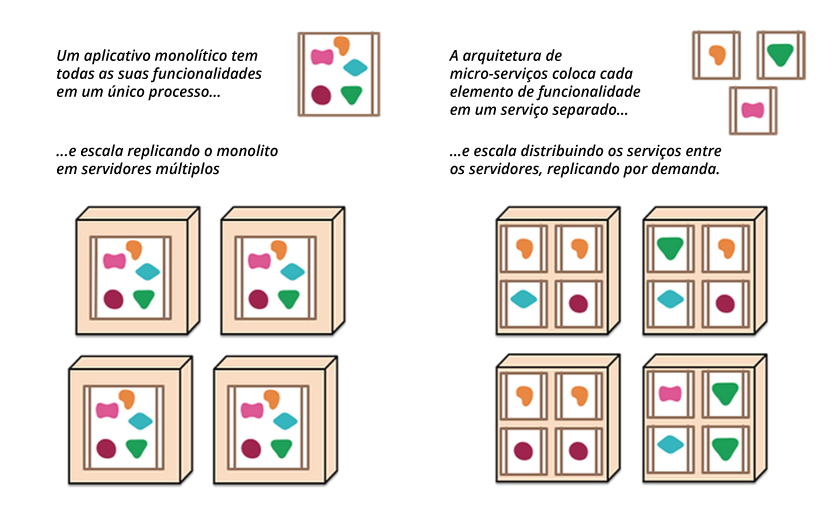
\includegraphics[width=0.8\linewidth]{imagens/1-arquitetura-microsservicos-fowler.png}    
    {\par \raggedright \footnotesize Fonte: \textcite{fowler_microsservicos_2022}\par}
\end{figure}

A arquitetura de microsserviços representa, portanto, um avanço em relação aos sistemas monolíticos tradicionais, promovendo a divisão dos serviços. Cada serviço possui sua própria base de dados, resultando na distribuição de dados por toda a arquitetura. De forma detalhada,conforme o entendimento de \textcite{lewis_microservices_2014}, enquanto o modelo monolítico centraliza tudo em um único bloco, a arquitetura de microsserviços distribui as responsabilidades em vários componentes menores e independentes. Essa abordagem promove escalabilidade, flexibilidade e resiliência em sistemas complexos e modernos.

A comunicação entre microsserviços, como já mencionado, ocorre predominantemente via \gls{api}s, \gls{http}, ou sistemas de mensagens assíncronas. A qualidade do design de comunicação é, portanto, determinante para a integração eficiente e a robustez do sistema, impactando diretamente o desempenho e a confiabilidade da solução. Proteger o tráfego de dados entre os serviços é essencial para assegurar a escalabilidade e a autonomia do sistema, além de atender às exigências rigorosas do setor econômico. Nesse contexto, é imprescindível adotar práticas de orquestração, monitoramento e documentação para visibilidade e controle sobre o comportamento dos serviços.

\subsection{Orquestração de Microsserviços}

Em arquiteturas de microsserviços, a \textbf{orquestração} refere-se à coordenação e gestão do ciclo de vida de múltiplos serviços independentes que colaboram para executar uma funcionalidade de negócio complexa \cite{newman_building_2022}. Em um sistema distribuído, como no nosso cenário de um assistente virtual multimodal, diferentes microsserviços precisam interagir de forma sequencial e eficiente. A escolha da tecnologia de orquestração é crucial para o desempenho, a latência e a resiliência do sistema. Este processo envolve a definição de como os serviços se comunicam, como os dados são serializados e como as chamadas são gerenciadas para garantir a entrega da funcionalidade completa ao usuário. A complexidade dos padrões de comunicação pode crescer exponencialmente com a adição de novos serviços, tornando o gerenciamento do sistema mais desafiador \cite{kleppmann_designing_2017}.

A orquestração eficaz é vital para mitigar os desafios inerentes aos microsserviços, como a complexidade de comunicação, a consistência de dados e a tolerância a falhas. Embora existam diversos protocolos de comunicação para sistemas distribuídos, desde comunicações tradicionais como WebSockets e Filas de Mensagens (MQTT) até soluções mais modernas como Apache Kafka\footnote{Disponível em https://kafka.apache.org. Acesso em 30/07/2025}, \acrshort{graphql}\footnote{Disponível em  https://graphql.org. Acesso em 30/07/2025} e Protocol Buffers, esta pesquisa concentra-se em três tecnologias que representam diferentes paradigmas arquiteturais e possuem sólida adoção na indústria\cite{jetbrains_state_2024}. A seleção de \gls{rest}, \gls{grpc} e Apache Thrift baseia-se em critérios específicos: (1) \gls{rest} representa o padrão consolidado e amplamente adotado em \gls{api}s web; (2) \gls{grpc} representa a evolução moderna com serialização binária e \acrshort{http}/2; e (3) Apache Thrift oferece uma alternativa madura com foco em performance e interoperabilidade entre linguagens. Essa escolha permite uma análise comparativa abrangente que cobre tanto soluções já estabelecidas quanto tecnologias emergentes, trazendo \textit{insights} práticos para decisões arquiteturais em contextos reais. A \autoref{tab:2-protocolos} apresenta uma comparação desses três protocolos de comunicação que serão avaliados nesse estudo, destacando suas características principais no contexto de comunicação e detalhando cada uma nas seções a seguir.

\begin{table}[H]
\caption{Comparativo de Protocolos de Comunicação para Orquestração de Microsserviços}
\centering
\begin{tabularx}{\textwidth}{|X|c|c|c|}
\hline
\textbf{Característica} & \textbf{\gls{rest}} & \textbf{\gls{grpc}} & \textbf{Thrift} \\
\hline
Comunicação & \acrshort{http}/1.1, \acrshort{http}/2 & \acrshort{http}/2 & \acrshort{tcp} \\
\hline
Serialização & \acrshort{json}, \acrshort{xml} & Protocol Buffers & Formato binário próprio \\
\hline
Tipo & Requisição/Resposta & Streaming & Requisição/Resposta \\
\hline
Binário & Não binário & .proto & .thrift \\
\hline
\end{tabularx}
\label{tab:2-protocolos}
\vspace{-0.2cm}
{\raggedright \footnotesize Fonte: Elaborado pelo autor.\par}
\end{table}

\subsubsection{\acrfull{rest}}

\gls{rest} constitui um padrão de comunicação amplamente adotado para o desenvolvimento de \gls{api}s web, fundamentado nos princípios do protocolo \gls{http}. Sua popularidade deriva da simplicidade, diversidade e utilização de padrões web, que facilitam a integração e o consumo em diversas plataformas \cite{mozilla_rest_2023}. Para a orquestração de microsserviços, \gls{rest} emprega requisições \gls{http} (GET, POST, PUT, DELETE) com o intuito de interagir com recursos, frequentemente utilizando payloads no formato \acrshort{json}. A natureza stateless do \gls{rest} simplifica o design dos serviços, pois cada requisição contém todas as informações necessárias para seu processamento, favorecendo, portanto, a escalabilidade horizontal. Entretanto, essa abordagem pode induzir bloqueios nos serviços até que a resposta seja recebida e requer que cada serviço conheça a localização dos demais, frequentemente necessitando de mecanismos de descoberta de serviços. A serialização textual (\acrshort{json}) e a sobrecarga do protocolo \gls{http}/1.1 podem também resultar em aumento de latência e consumo de banda em cenários com grandes volumes de dados ou que demandam alta performance \cite{mozilla_rest_2023}.

\subsubsection{\acrfull{grpc}}

O \acrshort{grpc} é um \textit{framework} de \acrfull{rpc} de código aberto, desenvolvido pelo Google, que utiliza \acrshort{http}/2 como protocolo de transporte e \textit{Protocol Buffers} como formato de serialização de dados \cite{google_grpc_nodate}. Diferente do \acrshort{rest}, que é orientado a recursos, o \acrshort{grpc} é orientado a serviços e métodos, permitindo a definição de contratos de serviço rigorosos por meio de arquivos \texttt{.proto}. O compilador de \textit{Protocol Buffers} processa esses arquivos para gerar automaticamente código cliente e servidor - conhecidos como \textit{bindings} - em múltiplas linguagens de programação.

\begin{figure}[H]
    \caption{Fluxo de comunicação gRPC entre clientes (Go/Ruby) e um serviço gRPC.}
    \label{fig:2-grpc-fluxo}
    \centering
    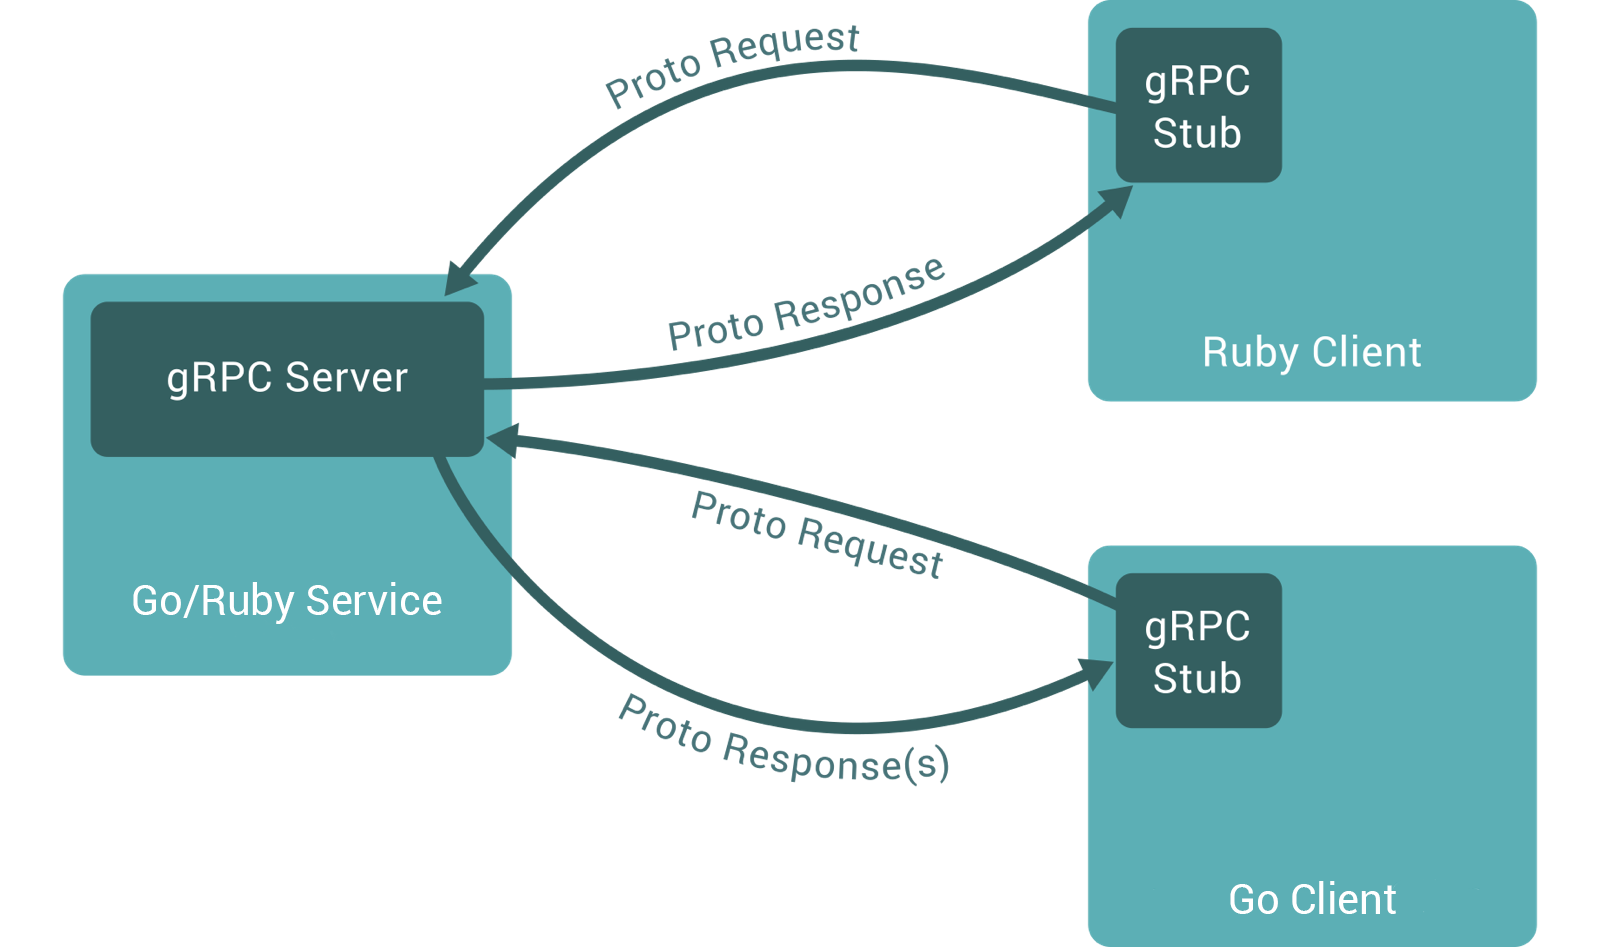
\includegraphics[width=0.5\linewidth]{imagens/2-gRPC-Flow.png}    
    {\par \raggedright \footnotesize Fonte: \textcite{google_grpc_nodate}.\par}
\end{figure}

Esses \textit{bindings} são fortemente tipados porque preservam toda a estrutura de dados e assinaturas de métodos definidas no contrato \texttt{.proto}, permitindo verificação de tipos em tempo de compilação e evitando erros comuns de serialização. A abordagem, combinada com a serialização binária e a multiplexação do \acrshort{http}/2, resulta em menor latência e maior \textit{throughput}, tornando-o ideal para comunicação interna entre microsserviços, nos quais a eficiência é importante. A geração automática de \textit{bindings multiplataforma} permite que serviços desenvolvidos em diferentes linguagens (como \textit{Go, Python, Java, C\#}) se comuniquem de forma transparente e eficiente, garantindo interoperabilidade em ambientes heterogêneos, conforme ilustrado na \autoref{fig:2-grpc-fluxo}. No entanto, o \acrshort{grpc} pode apresentar uma curva de aprendizado maior para clientes acostumados com \acrshort{rest} e possui uma especificação mais estrita, com menor suporte a outros tipos de conteúdo fora do \textit{Protobuf}.

\subsubsection{Apache Thrift}

O Apache Thrift é um \textit{framework} de \gls{rpc} e serialização de dados desenvolvido originalmente pelo Facebook e posteriormente incorporado ao ecossistema Apache. Sua arquitetura foi projetada especificamente para permitir comunicação eficiente entre serviços implementados em diferentes linguagens de programação \cite{apache_apache_nodate}.

A base do Thrift consiste em uma \textit{Interface Definition Language} (IDL) própria, onde os desenvolvedores definem os contratos de serviço em arquivos .thrift. Esses arquivos descrevem estruturas de dados, interfaces de serviço e exceções de forma independente de linguagem. O compilador Thrift então gera automaticamente o código correspondente na linguagem-alvo, produzindo \textit{bindings} fortemente tipados que garantem segurança e consistência na comunicação entre os serviços.

Assim como o \gls{grpc}, o Thrift emprega serialização binária para eficiência no transporte de dados, mas difere em sua abordagem de transporte, suportando tanto HTTP quanto TCP puro. Essa flexibilidade permite otimizações específicas para diferentes cenários de uso. O framework é particularmente adequado para ambientes heterogêneos onde serviços escritos em linguagens distintas (como Java, Python, C++, Ruby) precisam se comunicar com desempenho próximo ao de chamadas locais.

Entre suas principais vantagens destacam-se a baixa sobrecarga (\textit{overhead}) na serialização, suporte a tipos de dados complexos e a capacidade de trabalhar com conexões persistentes. No contexto de microsserviços, o Thrift se mostra uma alternativa robusta para cenários que exigem baixa latência e alta vazão, especialmente em implementações onde o controle fino sobre a camada de transporte é necessário \cite{apache_apache_nodate}.

\subsection{Desempenho e Escalabilidade}

O desempenho de um sistema refere-se à capacidade de responder de forma rápida e eficiente às solicitações dos usuários. Em arquiteturas de microsserviços, essa performance é impactada pela comunicação entre os serviços. O acoplamento solto da arquitetura permite o dimensionamento autônomo de cada serviço, distribui a carga de trabalho e reduz gargalos. Dessa forma, é possível aplicar técnicas como caching, balanceamento de carga e otimização dos tempos de resposta, fundamentos para manter o sistema responsivo sob alta demanda \cite{newman_building_2022}.

Em sistemas distribuídos, a latência da rede na comunicação entre serviços é um fator crítico. Para mitigar esse impacto e aproveitar plenamente os benefícios de sistemas resilientes e de baixa latência, é crucial investir em um design cuidadoso das interfaces e na implementação de mecanismos de resiliência, como circuit breakers, que monitoram falhas e, ao detectarem uma taxa elevada de erros, interrompem temporariamente as requisições ao serviço problemático. Essa abordagem evita falhas em cascata e permite a recuperação do serviço \cite[p. 131]{kleppmann_designing_2017}. 

A escalabilidade, por sua vez, é definida como a capacidade de um sistema crescer e se adaptar ao aumento da demanda \cite[p. 60]{fowler_microsservicos_2022}, e é um dos pilares que impulsionam a adoção de microsserviços. Conforme \cite{newman_building_2022}, a arquitetura de microsserviços facilita a escalabilidade horizontal, permitindo a adição ou remoção de instâncias de um serviço específico em resposta à demanda, em vez de replicar toda a aplicação. Essa granularidade assegura uma utilização de recursos mais eficiente e econômica, especialmente em ambientes de nuvem. A combinação de escalabilidade, resiliência e desempenho otimizado torna a arquitetura de microsserviços um modelo robusto para sistemas complexos e dinâmicos, como as aplicações no setor financeiro.
\vspace{\fill}
\subsection{Observabilidade e Monitoramento}

A arquitetura de microsserviços, embora traga benefícios significativos em flexibilidade e escalabilidade, introduz uma complexidade inerente devido à natureza distribuída e interconectada de seus componentes. Nesse cenário, a observabilidade e o monitoramento tornam-se cruciais para garantir a resiliência e a disponibilidade dos sistemas, especialmente em ambientes de alta criticidade como o setor financeiro \cite{arditti_microsservicos_2025}. A observabilidade pode ser definida como a capacidade de inferir o estado interno de um sistema a partir de seus dados externos, permitindo compreender e diagnosticar seu comportamento de forma eficaz. Práticas robustas de monitoramento, por sua vez, possibilitam a detecção rápida de problemas, como falhas de serviço, lentidão e sobrecarga, favorecendo respostas ágeis e a manutenção da estabilidade operacional \cite[p. 156]{fowler_microsservicos_2022}

Para alcançar uma observabilidade abrangente em microsserviços, é fundamental coletar e analisar três pilares de telemetria: métricas, logs e rastreamento distribuído. Métricas fornecem dados quantitativos sobre o desempenho do sistema (ex: utilização de CPU, memória, latência, throughput), enquanto os logs registram eventos e estados dos serviços, sendo essenciais para depuração e auditoria. O rastreamento distribuído, por sua vez, permite acompanhar o fluxo completo de uma requisição através de múltiplos microsserviços, identificando gargalos e falhas em cadeias de execução complexas  \cite{ibm_o_2023}. Ferramentas como Prometheus\footnote{Disponível em: \url{https://prometheus.io/}. Acesso em: 17 de jul. 2025.} e Grafana\footnote{Disponível em: \url{https://grafana.com/}. Acesso em: 17 de jul. 2025.} para métricas, o Elastick Stack\footnote{Disponível em: \url{https://www.elastic.co/elastic-stack/}. Acesso em: 17 de jul. 2025.} para logs e Jaeger\footnote{Disponível em: \url{https://www.jaegertracing.io/}. Acesso em: 17 de jul. 2025.} ou Zipkin\footnote{Disponível em: \url{https://zipkin.io/}. Acesso em: 17 de jul. 2025.} para rastreamento distribuído são comumente empregadas para consolidar e visualizar esses dados.

No contexto do mercado financeiro, a observabilidade inteligente é vital para prevenir problemas e proteger operações sensíveis, onde a integridade e a agilidade são indispensáveis. Um monitoramento preciso e em tempo real da stack de microsserviços garante que nenhuma métrica ou rastreamento importante seja perdido, fornecendo informações gerenciais precisas às equipes de DevOps e aumentando o tempo de resposta para prevenção e triagem de incidentes \cite{baumgartner_observabilidade_2024}.
% -- Assistentes Virtuais
\section{Assistentes virtuais}

Assistentes virtuais são sistemas computacionais projetados para interagir com seres humanos de forma natural, simulando comunicação e execução de tarefas via interfaces digitais \cite{cruz_assistentes_2018}. Seu objetivo principal é facilitar o acesso à informação, automatizar processos, responder perguntas, realizar comandos e oferecer suporte personalizado em diversos contextos, desde o atendimento ao cliente até a automação residencial e corporativa. A \autoref{fig:funcionamento-assistente} esquematiza o funcionamento simplificado de um assistente virtual.


\begin{figure}[H]
    \caption{Funcionamento simplificado de um assistente virtual.}
    \label{fig:funcionamento-assistente}
    \centering
    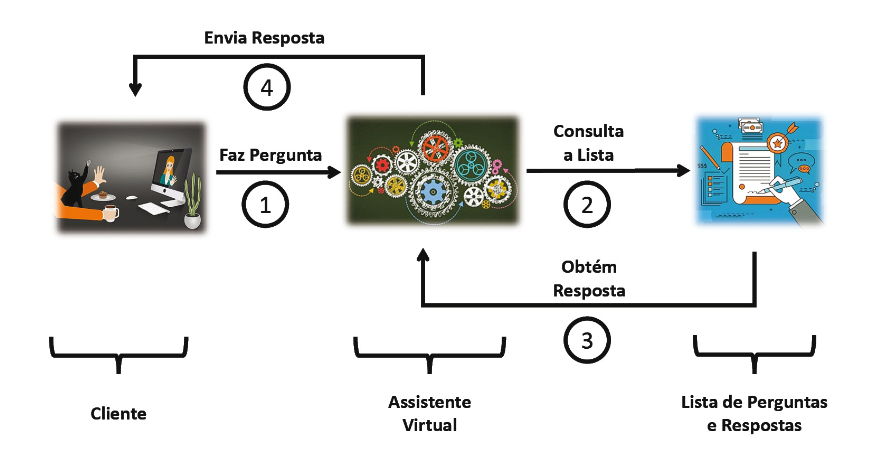
\includegraphics[width=\linewidth, height=8cm]{imagens/2-funcionamento-assistente-virtual.png}    
    {\par \raggedright \footnotesize Fonte: \textcite{cruz_assistentes_2018}.\par}
\end{figure}



A arquitetura de um assistente virtual é composta por diferentes módulos especializados, que trabalham de forma integrada para compreender, processar e responder às solicitações dos usuários. Os principais componentes incluem:

\begin{itemize}
  \item \textbf{Reconhecimento de fala (Speech-to-Text)}: Converte comandos de voz em texto, permitindo que o assistente compreenda solicitações verbais.
    \item \textbf{Processamento de linguagem natural (Text-to-Text)}: Interpreta o texto recebido, identifica intenções, extrai entidades e gera respostas adequadas.
    \item \textbf{Síntese de fala (Text-to-Speech)}: Transforma textos em áudio, possibilitando respostas em voz natural.
    \item \textbf{Módulos de integração}: Conectam o assistente a sistemas externos, bancos de dados, \gls{api}s e dispositivos inteligentes.
    \item \textbf{Gestão de contexto}: Mantém o histórico de interações, permitindo diálogos contínuos e personalizados.
\end{itemize}

Os assistentes virtuais são impulsionados por um conjunto de tecnologias de \acrfull{ia}, nas quais sistemas de \gls{ml} e \gls{dl} possibilitam o reconhecimento de padrões em voz e linguagem, bem como a personalização de interações, enquanto a própria \gls{ia} viabiliza a compreensão semântica e a tomada de decisão. Um marco revolucionário nessa área foi a introdução da arquitetura Transformer em 2017 \cite{vaswani_attention_2017}, que transformou o \gls{nlp} por meio de mecanismos de atenção — base dos atuais \gls{llm}, como ChatGPT e Gemini, conforme ilustrado na \autoref{fig:transformers}. A integração desses \gls{llm} generativos elevou substancialmente a capacidade de processamento de linguagem natural, permitindo a interpretação de nuances, a geração criativa de respostas e a adaptação contextual do tom comunicativo. Como resultado, ampliaram-se significativamente as aplicações práticas desses sistemas, que passaram a abranger desde atendimento automatizado e suporte técnico até a criação de conteúdo estruturado e a análise de dados complexos \cite{mckinsey_economic_2023}.

Nesse contexto, os assistentes virtuais consolidam-se como ferramentas interativas inovadoras, que utilizam \gls{nlp} e \gls{ia} para estabelecer comunicação direta e intuitiva com os usuários. Por meio de comandos de voz ou texto, tais sistemas respondem a perguntas, executam operações financeiras e oferecem orientações personalizadas — cobrindo desde demandas cotidianas até tarefas de maior complexidade, como recomendações de investimentos e simulações de crédito \cite{cruz_assistentes_2018}.

\begin{figure}[H]
    \caption{Evolução dos modelos de conversação.}
    \label{fig:transformers}
    \centering
    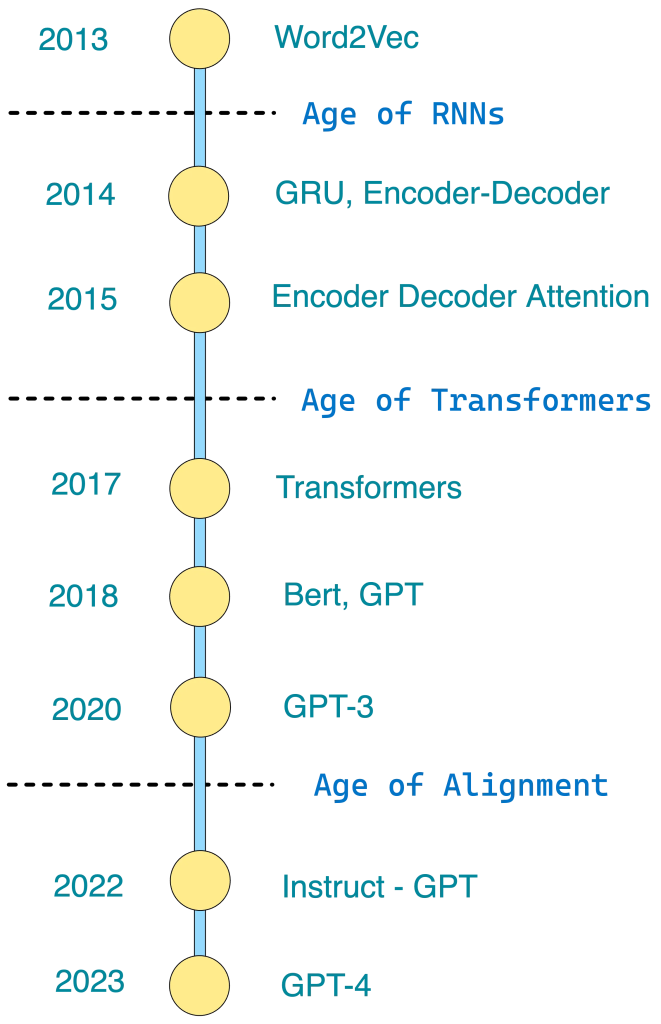
\includegraphics[width=0.3\linewidth]{imagens/4-transformers.png}    
    {\par \raggedright \footnotesize Fonte: \textcite{dsacademy_llms_2023}.\par}
\end{figure}

Apesar dos avanços, a adoção de grandes modelos de \gls{ia} generativa apresenta desafios significativos relacionados ao consumo intensivo de recursos computacionais e ao impacto na latência do sistema. Estudos acadêmicos demonstram que o treinamento de modelos como o GPT-3 demanda aproximadamente 1.287 megawatt-horas (MWh), equivalente ao consumo anual médio de 420 pessoas \cite{argerich_measuring_2024}. Durante a inferência, pesquisas mostram que modelos como o Bloom consomem aproximadamente 3,96 watt-horas por requisição \cite{argerich_measuring_2024}, enquanto aplicações como ChatGPT podem demandar mais de 1.500 MWh mensalmente considerando 13 milhões de usuários diários. A latência e o tempo de resposta são diretamente afetados pela complexidade dos modelos, onde a relação entre número de parâmetros e operações computacionais (aproximadamente duas vezes o número de parâmetros por token gerado) impacta significativamente o desempenho \cite{argerich_measuring_2024}, podendo comprometer a experiência do usuário em aplicações que requerem respostas em tempo real, especialmente no setor financeiro onde a rapidez de processamento é crítica para operações sensíveis ao tempo.


\subsection{Aplicações de Assistentes Virtuais baseadas em microsserviços no setor financeiro}

Nos últimos anos, o setor financeiro tem desenvolvido soluções tecnológicas sofisticadas que integram assistentes virtuais a complexos bancos de dados e arquiteturas distribuídas. Essas implementações incluem plataformas de análise preditiva para avaliação de crédito e detecção de fraudes, sistemas de automação de \textit{back-office}, e soluções de personalização que utilizam \gls{llm} e \gls{ia} Multimodal para enriquecer a análise de dados financeiros \cite{febraban_estudo_2024}. O investimento massivo nessas tecnologias reflete a busca por maior eficiência operacional e redução de custos, com a tecnologia sendo vista como um grande diferencial competitivo entre as instituições bancárias.

Essa convergência entre assistentes virtuais inteligentes e arquiteturas de microsserviços redefine a prestação de serviços financeiros, criando um ecossistema tecnológico ágil, escalável e eficiente. Estudos recentes da Febraban em colaboração com a Accenture demonstram que a \gls{ia} Generativa pode aumentar a eficiência dos bancos entre 25\% e 35\% \cite{febraban_estudo_2024}, enquanto pesquisa da IBM indica que a adoção estratégica dessa tecnologia pode elevar significativamente o desempenho financeiro das instituições \cite{ibm_2025_2025}. Esta transformação é particularmente relevante em um contexto onde microsserviços permitem desenvolvimento, otimização e dimensionamento independente de cada etapa do processamento de \gls{ia}, desde o pré-processamento de dados até a inferência de modelo e pós-processamento \cite{nvidia_decodificando_2024}.

No Brasil, exemplos práticos demonstram a maturidade dessa abordagem arquitetural. A \textbf{Bia (Bradesco Inteligência Artificial)} atende 3 milhões de clientes como assistente virtual multimodal, processando milhões de interações mensais sobre produtos financeiros através de múltiplos canais \cite{valor_investe_os_2025}. O \textbf{Banco do Brasil} desenvolveu a ferramenta "Ari" (Área de Recomendações Inteligentes), que já gerou mais de 60 milhões de recomendações personalizadas, impactando 2,5 milhões de micro e pequenos empresários com insights sobre volume de vendas, produtos financeiros e detecção de inadimplência \cite{valor_investe_os_2025}. Paralelamente, \textit{fintechs} como a \textbf{Magnetis} utilizam arquiteturas distribuídas para oferecer consultoria de investimentos automatizada, enquanto a \textbf{Accountfy} implementou assistentes virtuais com \gls{ia} integrados em sua plataforma SaaS para otimizar a governança financeira empresarial \cite{accountfy_assistentes_2024}.

A capacidade desses assistentes de interpretar e executar comandos em tempo real os torna ideais para bancos e \textit{fintechs} que buscam atendimento de alta qualidade e redução de custos operacionais. A arquitetura de microsserviços, comumente aplicada, permite que os assistentes integrem múltiplos módulos de dados de forma independente e escalável, aumentando a eficiência e facilitando a personalização de serviços \cite{villamizar_evaluating_2023}. A Interface desses sistemas se foca na interação por voz, visando uma comunicação mais natural e eficiente entre usuário e sistema, acompanhando o advento de ambientes tecnológicos cada vez mais conectados e sofisticados.

\chapter{Estado da Arte e Trabalhos Relacionados}
\label{ch:3estado_da_arte}

Neste capítulo, apresenta-se o mapeamento da literatura realizado no âmbito desta pesquisa, conduzido por meio de uma \acrfull{rsl}, seguindo as diretrizes metodológicas propostas por \textcite{scannavino_revisao_2017}. O objetivo central desta revisão consiste em identificar, avaliar e sintetizar os principais estudos publicados sobre a aplicação de arquiteturas de microsserviços em sistemas de \acrfull{ia}, com ênfase especial em aspectos de orquestração e desempenho. Para tanto, foram estabelecidos protocolos rigorosos de busca, seleção e análise de trabalhos, delimitando-se o escopo temático e definindo critérios de elegibilidade que garantissem a relevância e a qualidade científica dos materiais incluídos.

A revisão concentra-se particularmente em investigações que abordam avaliações experimentais de desempenho, testes comparativos de protocolos e métricas de eficiência em comunicações entre serviços, assegurando que a análise aprofunde questões diretamente relacionadas aos objetivos desta dissertação. A \autoref{sec:3-rsl} detalha o processo de revisão sistemática, descrevendo as etapas percorridas, os critérios de inclusão e exclusão adotados e os resultados obtidos em cada fase. Na \autoref{sec:3-sintese-trabalhos}, procede-se à análise crítica dos trabalhos selecionados, discutindo suas contribuições, limitações e relações com o contexto experimental aqui proposto, de modo a posicionar esta pesquisa no estado da arte e justificar sua originalidade e relevância.

\section{Revisão Sistemática da Literatura}
\label{sec:3-rsl}

Baseando-nos nas técnicas apresentadas por \textcite{scannavino_revisao_2017} e nos objetivos e na área de estudo delimitados no \autoref{ch:2pilares}, formulamos algumas questões de pesquisa para nortear a revisão sistemática da literatura. Essas questões visam identificar trabalhos relevantes já publicados na área, que são considerados referências de estado da arte para esta pesquisa. Estas perguntas são:

\begin{enumerate}
    \item  Como orquestrar microsserviços de modelos de \gls{ia} generativa?
    \item  Quais técnicas e métodos são discutidos para a orquestração desses microsserviços?
    \item  Qual tecnologia é mais adequada para suportar uma alta demanda de trabalho na orquestração de microsserviços?
\end{enumerate}

\subsection{Estratégia de Busca}

\textbf{BASE DE DADOS}: A estratégia de busca foi planejada para cobrir as principais bases de dados acadêmicas e motores de busca reconhecidos nas áreas de Engenharia de Software e \acrfull{ia}, assegurando uma abrangente cobertura da literatura científica. As plataformas selecionadas, destacadas por sua relevância e pelo volume de publicações qualificadas, incluem:
\begin{itemize}
    \item ABCD PBI (\url{https://www.buscaintegrada.usp.br/}): portal de buscas integrado da rede de pesquisa da USP e demais parceiros incluindo CAPES e outras instituições internacionais.
    \item Science Direct (\url{www.sciencedirect.com}): Uma das maiores bases de dados de literatura científica e técnica, com forte presença em engenharia e computação.
    \item IEEE Xplore (\url{ieeexplore.ieee.org}): Base de dados do Institute of Electrical and Electronics Engineers, crucial para publicações em engenharia, eletrônica e computação.
\end{itemize}

\textbf{STRING DE BUSCA}: A estratégia de busca foi construída a partir de um conjunto de palavras-chave em inglês e português, selecionadas para alinhar-se diretamente ao escopo desta dissertação. Utilizando operadores booleanos (AND, OR), buscou-se equilibrar abrangência e especificidade, refinando os resultados para o tema central — desempenho e orquestração de microsserviços em sistemas de \acrfull{ia} aplicados ao setor financeiro. Essa abordagem permitiu capturar a literatura mais relevante, majoritariamente internacional, sem perder de vista contribuições regionais significativas. As strings incluíram combinações como:

\begin{itemize}
\item "microservices" AND "AI models" AND "communication" AND ("benchmark" OR "comparison" OR "study")
\item "microservices" AND "orchestration" AND ("REST" OR "gRPC" OR "Apache Thrift") AND "benchmark"
\item "conversational agents" AND "microservices architecture"
\item "microservices" AND "AI models" AND "financial"
\end{itemize}

\textbf{RESULTADOS INICIAIS}: Estabeleceu-se como critério de triagem inicial a análise de \textbf{títulos e resumos (abstracts)} dos estudos recuperados pelas strings de busca, complementado por um filtro temporal que abrangeu o período de 2020 a 2025 para garantir a contemporaneidade dos trabalhos selecionados. Esta estratégia permitiu capturar as evoluções mais recentes nas tecnologias de microsserviços e \gls{ia}. Do volume inicial de documentos identificados, procedeu-se à eliminação de duplicatas, resultando em um corpus preliminar de \textbf{278 publicações únicas} para avaliação de elegibilidade nas etapas subsequentes.


\subsubsection{Critérios de Elegibilidade e Seleção}

Após a escolha das bases dados e definição das strings de busca, definiu-se um processo de filtragem e seleção dos trabalhos. Este processo de seleção dos estudos seguiu 4 etapas detalhadas a seguir, assegurando a inclusão apenas dos trabalhos mais relevantes e de alta qualidade científica:
\begin{enumerate}
\item \textbf{Identificação}: Nesta fase inicial, foram realizadas as buscas nas bases de dados utilizando as strings de pesquisa definidas. O objetivo foi coletar o maior número possível de documentos potencialmente relevantes.
\item \textbf{Triagem}: Os resultados brutos foram armazenados em uma ferramenta de gestão de referências chamada Zotero\footnote{Disponível em: \url{https://zotero.org/}. Acesso em: 29 ago. 2025.} para facilitar a organização. Em seguida, as duplicatas foram removidas. Uma primeira filtragem foi realizada através da leitura dos títulos, descartando artigos que claramente não se alinhavam ao tema. Além disso, apenas artigos publicados em periódicos avaliados por pares foram selecionados, demonstrando assim a relevância já posta à prova por outros pesquisadores.
\item \textbf{Seleção Inicial}: Os títulos e resumos dos documentos restantes foram lidos para uma avaliação mais aprofundada da relevância. Nesta etapa, foram selecionados os estudos que apresentavam uma possível interseção com os objetivos e questões de pesquisa, mesmo que de forma preliminar.
\item \textbf{Seleção Final}: A leitura completa dos artigos selecionados na etapa anterior foi realizada para verificar a interseção direta e aprofundada com os objetivos e questões de pesquisa desta dissertação. A qualidade metodológica e a contribuição científica de cada estudo foram avaliadas rigorosamente.
\end{enumerate}

\begin{table}[H]
\centering
\caption{Resultados das buscas utilizando os termos nas fontes definidas}
\begin{tabularx}{\textwidth}{|c|X|c|c|c|}
\hline
\textbf{Ordem} & \textbf{Termos da Pesquisa} & \textbf{PBi} & \textbf{IEEEx} & \textbf{Science Direct} \\
\hline
1 & "microservices" AND "AI models" AND "communication" AND ("benchmark" OR "comparison" OR "study") & 218 & 4 & 0 \\
\hline
2 & "microservices" AND "orchestration" AND ("REST" OR "gRPC" OR "Apache Thrift") AND "benchmark" & 195 & 2 & 2 \\
\hline
3 & "conversational agents" AND "microservices architecture" & 12 & 0 & 2 \\
\hline
4 & "microservices" AND "AI models" AND "financial" & 86 & 3 & 1 \\
\hline
\multicolumn{2}{|r|}{\textbf{Total}} & \textbf{511} & \textbf{9} & \textbf{5} \\
\hline
\end{tabularx}
\label{tab:3-total-rsl}
\vspace{-0.3cm}
{\raggedright \footnotesize Fonte: Elaborado pelo autor.\par}
\end{table}


\textbf{Etapas}: As etapas para seleção dos estudos foram aplicados em diferentes etapas do processo de revisão:
\begin{itemize}
\item \textbf{Etapa inicial de buscas}: Os filtros de \textit{período (2020-2025)} e \textit{idioma (inglês ou português)} foram aplicados diretamente nas plataformas de busca durante a recuperação inicial dos documentos.

\item \textbf{Triagem por título e resumo}: Nestas etapas, avaliou-se preliminarmente a \textit{abordagem temática}, selecionando estudos que tratassem de aplicação de microsserviços em sistemas de \gls{ia} ou assistentes virtuais.

\item \textbf{Leitura integral}: A \textit{ênfase em aspectos específicos} (desempenho, orquestração, escalabilidade ou desafios de comunicação) foi criteriosamente verificada apenas através da leitura completa dos artigos, constituindo-se no filtro mais refinado do processo.
\end{itemize}

Foram excluídos os trabalhos que não se enquadravam no escopo, como artigos sobre \acrfull{ia} sem relação com microsserviços ou microsserviços que não abordassem desempenho ou orquestração. Além disso, consideraram-se não elegíveis os artigos duplicados, revisões sistemáticas ou surveys, priorizando-se estudos primários empíricos, ou aqueles que não apresentassem conteúdo científico revisado por pares, como preprints não revisados, postagens de blogs sem autoria acadêmica e whitepapers sem rigor científico.

\begin{figure}[H]
\centering
\caption{Processo de Revisão Sistemática da Literatura (Adaptado de \textcite{scannavino_revisao_2017})}
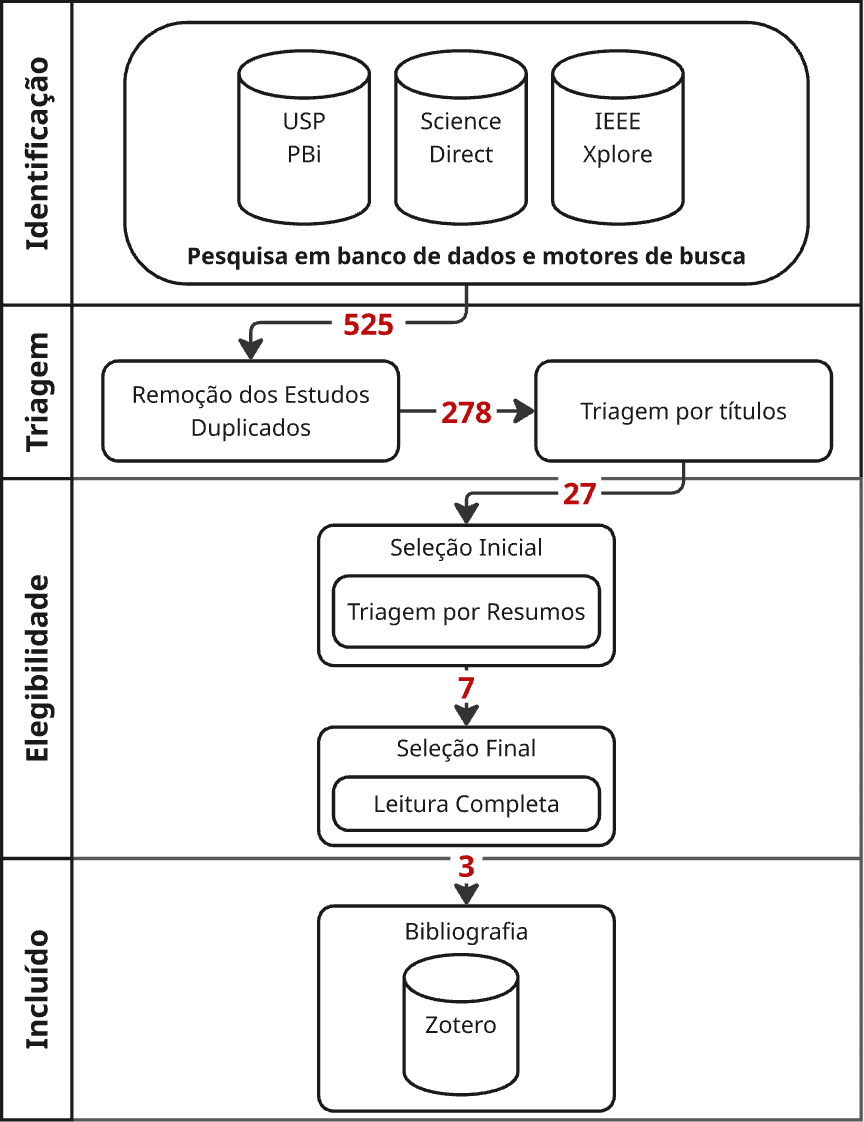
\includegraphics[width=0.65\textwidth]{imagens/3-revisao-literatura.png} 
\label{fig:rsl_process}
{\par \raggedright \footnotesize Fonte: Elaborado pelo autor.}
\end{figure}

A \autoref{fig:rsl_process} mostra o processo de seleção e triagem de documentos, que abrange desde a identificação inicial até a inclusão final. Por meio de métodos automatizados com o Zotero, o conjunto inicial foi reduzido a 278 documentos. A revisão dos títulos resultou na identificação de 27 estudos possivelmente relacionados ao tema. A análise dos títulos e resumos refinou a seleção para 7 estudos, dos quais 3 foram escolhidos após leitura aprofundada, devido à sua relevância direta para a pesquisa e ao seu destaque em relação aos demais artigos selecionados. Os números totais podem ser visualizados na \autoref{tab:3-total-rsl}.

A próxima seção examina os três artigos finais selecionados mediante uma análise crítica organizada em quatro dimensões principais: metodologia experimental (ambiente, ferramentas e cenários de teste), métricas de desempenho (latência, throughput, uso de recursos), motivação e objetivos, e conclusões e contribuições para a área. Essa abordagem multidimensional é estrategicamente alinhada aos objetivos desta pesquisa, uma vez que o exame detalhado das metodologias oferece insights para o desenho de nosso próprio ambiente de testes, a comparação das métricas possibilita a seleção das variáveis mais relevantes, a compreensão das motivações auxilia no posicionamento contextual de nossa contribuição, e a análise das conclusões fornece parâmetros comparativos para interpretar nossos resultados à luz do estado da arte. Dessa forma, esta seção não apenas sintetiza o conhecimento existente e estabelece um diálogo crítico entre os trabalhos identificando convergências e lacunas metodológicas, mas também fundamenta as escolhas metodológicas e analíticas adotadas neste trabalho.

\section{Síntese dos Principais Trabalhos Relacionados}
\label{sec:3-sintese-trabalhos}
% -- Niswar 2024
\subsection{Performance evaluation of microservices communication with \acrshort{rest}, \acrshort{graphql}, and \acrshort{grpc} \cite{niswar_performance_2024}}
\label{sec:3-niswar}

A pesquisa de \textcite{niswar_performance_2024} propõe uma avaliação e comparação abrangente do desempenho de três protocolos de comunicação amplamente utilizados em arquiteturas de microsserviços: \gls{rest}, \acrshort{graphql} e \gls{grpc}. O estudo concentra-se na troca de dados, abordando cenários de recuperação de dados planos e aninhados, com o objetivo de fornecer insights valiosos para que desenvolvedores e arquitetos possam otimizar a escolha dos protocolos de comunicação, considerando casos de uso e cargas de trabalho específicas.

O desafio da comunicação eficiente entre esses serviços independentes é um ponto central do trabalho. Embora os autores apontem o \gls{rest} como o método mais popular para troca de dados, eles argumentam que este protocolo apresenta desvantagens, como o over-fetching (recuperação de mais dados do que o necessário) e o under-fetching (recuperação de dados insuficientes, o que exige requisições adicionais). Nesse contexto, o \acrshort{graphql} surge como uma alternativa para superar tais ineficiências, permitindo que os clientes especifiquem exatamente os dados necessários. Já o \gls{grpc}, segundo os autores, destaca-se por sua abordagem eficiente e versátil na comunicação entre serviços distribuídos, utilizando o protocolo \acrshort{http}/2, que suporta streaming de dados e simplifica chamadas de procedimento remoto em diversas linguagens de programação.

Para realizar a avaliação, os autores estabeleceram um ambiente experimental composto por três microsserviços implementados em contêineres, cada um com um banco de dados Redis para cache em memória e MySQL para armazenamento persistente. O estudo utilizou dados de um Sistema Integrado de Informação Educacional, focando especificamente nas informações sobre o perfil dos professores e em seus históricos educacionais, abrangendo dados planos e aninhados. A metodologia de avaliação de desempenho empregou o Apache JMeter\footnote{Disponível em \hyperref[https://jmeter.apache.org]{https://jmeter.apache.org}} para simular testes de carga de \gls{api}, coletando métricas-chave como tempo de resposta e utilização da CPU. Foram realizadas duas abordagens de avaliação: requisições concorrentes e requisições consecutivas, com o número de requisições variando de 100 a 500, a fim de simular diferentes níveis de carga, conforme \autoref{fig:2-niswar-1}.

\begin{figure}[H]
    \caption{Cenário proposto por \textcite{niswar_performance_2024}}
    \label{fig:2-niswar-1}
    \centering
    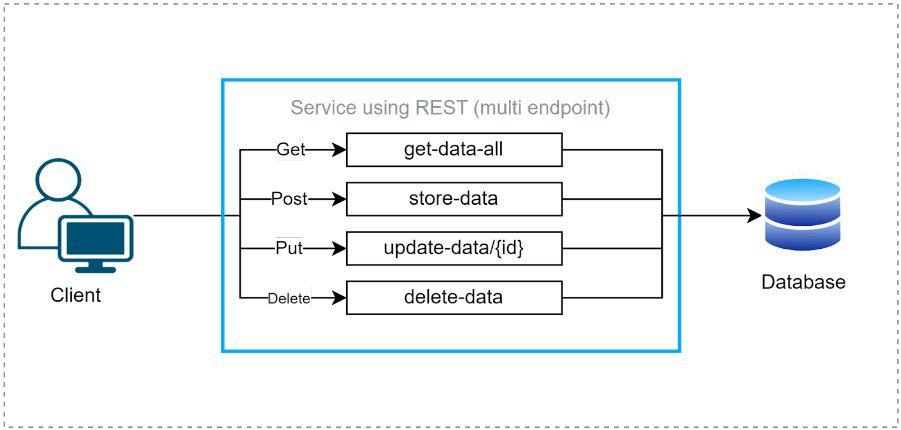
\includegraphics[width=0.75\linewidth]{imagens/niswar-1-enviroment.jpg}    
    {\par \raggedright \footnotesize Fonte: \textcite{niswar_performance_2024}.\par}
\end{figure}

Nos testes de requisições concorrentes, o tempo de resposta médio configurou-se como uma métrica crucial. Tanto para a recuperação de dados planos quanto aninhados, o \gls{grpc} demonstrou consistentemente tempos de resposta significativamente inferiores aos observados com \gls{rest} e \acrshort{graphql}. Por exemplo, para 100 requisições de dados planos, o \gls{grpc} foi aproximadamente 5 vezes mais rápido que o \gls{rest} e 16 vezes mais rápido que o \acrshort{graphql}. Essa vantagem de desempenho do \gls{grpc} manteve-se e intensificou-se à medida que o número de requisições aumentava, como pode ser observado nas figuras \ref{fig:2-niswar-time-flat} e \ref{fig:2-niswar-time-nested}.

Os resultados reforçam a eficiência do \gls{grpc} tanto para estruturas de dados simples quanto complexas e sob diferentes cargas, atribuída pelos autores ao uso do protocolo \acrshort{http}/2 e à serialização binária via Protocol Buffers.

\begin{figure}[htb]
  \centering
  \begin{minipage}[t]{0.48\linewidth}
    \caption{Tempos de respostas dos microsserviços com dados Flat}
    \label{fig:2-niswar-time-flat}
    \centering
    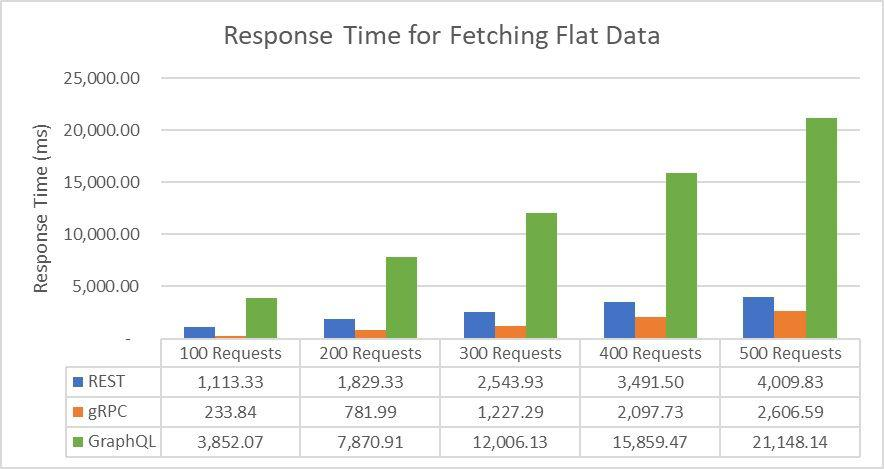
\includegraphics[width=\linewidth]{imagens/niswar_time_flat.jpg}    
    {\par \raggedright \footnotesize Fonte: \textcite{niswar_performance_2024}.\par}
  \end{minipage}%
  \hfill
  \begin{minipage}[t]{0.48\linewidth}
    \caption{Tempos de respostas dos microsserviços com dados Aninhados}
    \label{fig:2-niswar-time-nested}
    \centering
    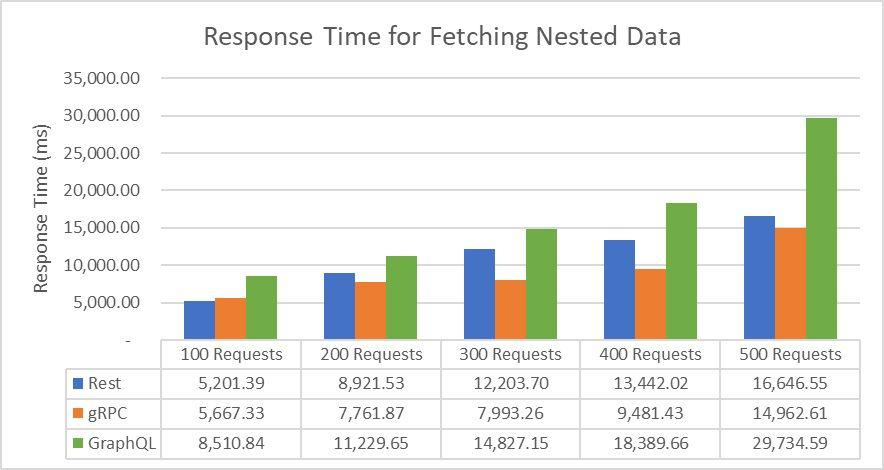
\includegraphics[width=\linewidth]{imagens/niswar_time_nested.jpg}    
    {\par \raggedright \footnotesize Fonte: \textcite{niswar_performance_2024}.\par}
  \end{minipage}
\end{figure}

Em relação à utilização da CPU, os resultados revelaram diferenças notáveis entre os protocolos, como ilustrado nas figuras \ref{fig:2-niswar-cpu-flat} e \ref{fig:2-niswar-cpu-nested}. Para a recuperação de dados planos, o protocolo \gls{rest} apresentou a menor utilização média da CPU, enquanto o \gls{grpc} mostrou consumo ligeiramente superior, porém ainda eficiente. Em contraste, o \acrshort{graphql} demonstrou uma utilização de CPU consideravelmente mais alta, frequentemente superando 100\%, o que, de acordo com os autores, indica uma demanda de recursos intensiva devido à complexidade inerente à análise e processamento de suas queries flexíveis.

Para a recuperação de dados aninhados, a tendência manteve-se semelhante: \gls{rest} e \gls{grpc} preservaram perfis de consumo mais eficientes, enquanto o \acrshort{graphql} novamente exigiu o maior esforço computacional, atingindo picos de utilização próximos a 180\% em cenários de maior carga. Esses padrões são visíveis nas figuras \ref{fig:2-niswar-cpu-flat} e \ref{fig:2-niswar-cpu-nested}, que detalham o comportamento dos protocolos sob diferentes volumes de requisições e complexidade de dados.

\begin{figure}[htb]
  \centering
  \begin{minipage}[t]{0.48\linewidth}
    \caption{Uso de CPU dos microsserviços com dados Flat}
    \label{fig:2-niswar-cpu-flat}
    \centering
    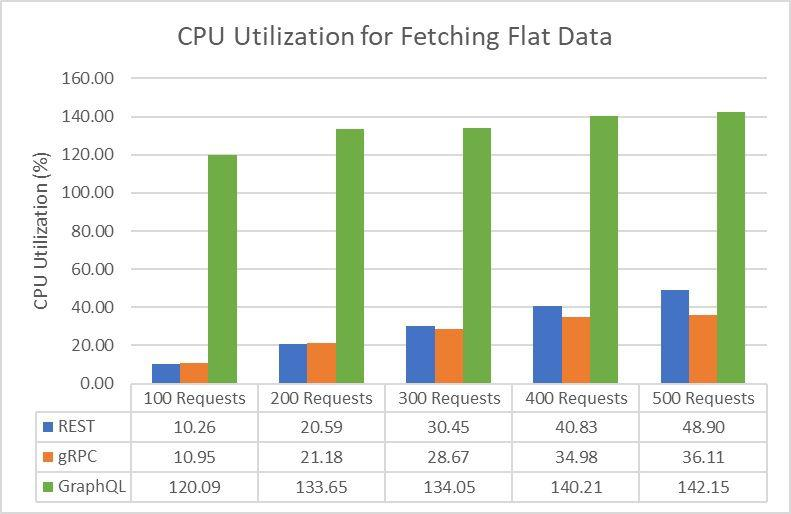
\includegraphics[width=\linewidth]{imagens/niswar_cpu_flat.jpg}    
    {\par \raggedright \footnotesize Fonte: \textcite{niswar_performance_2024}.\par}
  \end{minipage}%
  \hfill
  \begin{minipage}[t]{0.48\linewidth}
    \caption{Uso de CPU dos microsserviços com dados Aninhados}
    \label{fig:2-niswar-cpu-nested}
    \centering
    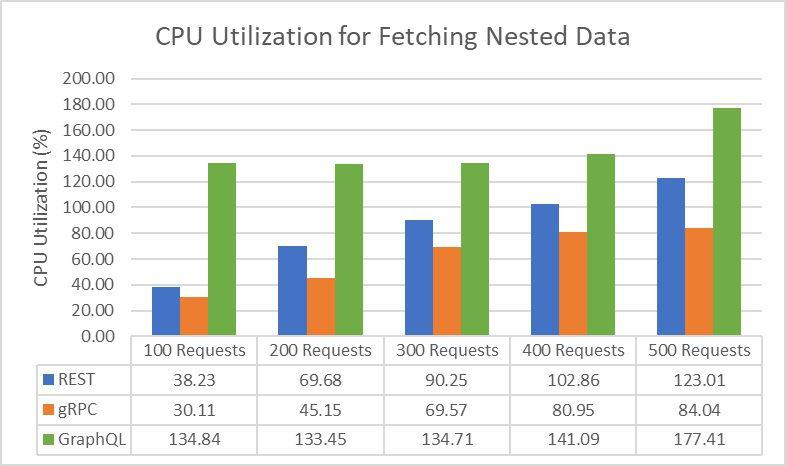
\includegraphics[width=\linewidth]{imagens/niswar_cpu_nested.jpg}    
    {\par \raggedright \footnotesize Fonte: \textcite{niswar_performance_2024}.\par}
  \end{minipage}
\end{figure}

A avaliação de requisições consecutivas, realizada durante cinco minutos e variando de 100 a 500 requisições, corroborou os achados dos testes concorrentes. O \gls{grpc} manteve-se como o protocolo com o tempo de resposta mais rápido para ambos os tipos de dados (flat e aninhados), evidenciando consistência sob diferentes padrões de carga. A capacidade do \gls{grpc} de utilizar o protocolo \acrshort{http}/2, que apresenta recursos como multiplexação (que permite múltiplas requisições sobre uma única conexão) e serialização binária eficiente (Protocol Buffers), é destacada pelos autores como o principal fator de seu desempenho superior em comparação ao \gls{rest} e ao \acrshort{graphql}.

\subsubsection{Resumo do Estudo}

Em suma, o estudo de \cite{niswar_performance_2024} conclui que o \gls{grpc} supera o \gls{rest} e o \acrshort{graphql} em termos de tempo de resposta, configurando-se como a escolha mais eficiente para comunicação em microsserviços que demandam baixa latência. Por outro lado, o \gls{rest} demonstrou menor utilização da CPU em alguns cenários, o que pode ser um fator relevante em ambientes com restrições de recursos. Embora o \acrshort{graphql} ofereça flexibilidade na recuperação de dados, resulta em maior consumo de CPU e aumento no tempo de resposta. As descobertas proporcionam insights práticos para a escolha de protocolos de \gls{api} em ambientes de microsserviços, levando em consideração os requisitos específicos de cada caso de uso e carga de trabalho.
% -- Maulana 2022
\vspace{\fill}
\subsection{Design and Testing on Migration of Remiss-Supply in Banking System to Microservice Architecture \cite{maulana_design_2022}}

\label{subsec:maulana_design}

\textcite{maulana_design_2022} apresentam um estudo focado na migração arquitetural de um sistema bancário monolítico para uma arquitetura de microsserviços, especificamente para o serviço de Remiss Supply do PTBank Indonesia. A principal motivação para a migração, conforme destacado pelos autores, reside na superação das limitações das arquiteturas monolíticas tradicionais, que apresentam falta de flexibilidade, dificuldades de manutenção e suscetibilidade a falhas em cadeia.

Foram utilizados como base do estudo os subserviços do sistema proprietário Remiss Supply, descritos pelo pesquisador em seu trabalho e visíveis na ilustração \autoref{fig:3-maulana-scenario}. Os três sistemas analisados foram:

\begin{itemize}
    \item \textbf{Inquiry Data}: Responsável por realizar buscas e consultas de dados completos de transações históricas, permitindo o rastreamento de atividades de depósito e retirada com base em parâmetros como datas de recebimento, entrega, identificação da agência e ID da transação;
    
    \item \textbf{Inquiry Details}: Especializado em fornecer informações detalhadas e específicas sobre transações, incluindo denominações de cédulas e dados complementares que aprofundam a análise das operações realizadas;
    
    \item \textbf{Remis Supply Request}: Gerencia solicitações de novas transações de retirada e depósito, processando casos de "REMIS" (depósitos em numerário) e "SUPPLY" (retiradas em numerário), incluindo validações, conexões com serviços centrais e persistência de dados transacionais;
\end{itemize} 

O processo de migração do serviço do banco foi segmentado em sprints, com foco na análise do sistema monolítico, no design do banco de dados, na coleta de recursos, na criação de esquemas \gls{xml} para requisições e respostas, e na implementação do código para os microsserviços. Por fim, realiza-se a implantação em contêineres Docker\footnote{Disponível em https://www.docker.com/} e máquinas virtuais, utilizando a linguagem de programação Java\footnote{Disponível em https://www.java.com/} na implementação.

\begin{figure}
    \caption{Cenário descrito nos testes}
    \label{fig:3-maulana-scenario}
    \centering
    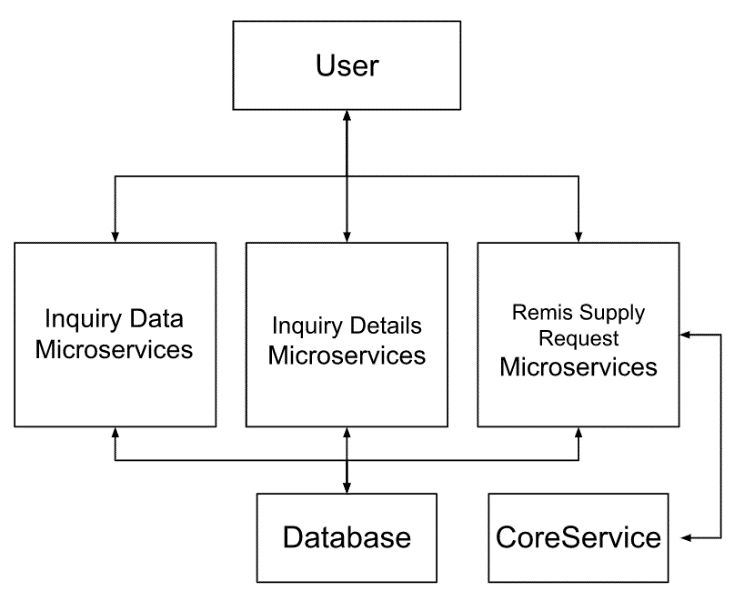
\includegraphics[width=0.5\linewidth]{imagens/maulana_scenario.jpg}    
    {\par \raggedright \footnotesize Fonte: \textcite{maulana_design_2022}.\par}
\end{figure}

Os testes de desempenho foram realizados para comparar as arquiteturas monolítica e de microsserviços sob diferentes condições de carga e estresse, incluindo variações no número de requisições simultâneas e cenários de alta (Ver \autoref{tab:3-maulana-testes-carga}) concorrência, utilizando o tempo de resposta, a latência e o \textit{throughput} como métricas principais. 

\begin{table}[H]
\centering
\caption{Condições de carga e estresse}
\label{tab:3-maulana-testes-carga}
\makebox[\textwidth][c]{%
\begin{tabularx}{\textwidth}{|l|X|}
\hline
\textbf{Condições de carga} & Throughput de 200 e 1.000 threads por minuto. \\
\hline
\textbf{Condições de estresse (microsserviços)} & \textit{Ramp-up} de 1 a 1.000 threads. \\
\hline
\end{tabularx}%
}
{\par \raggedright \footnotesize Fonte: \textcite{maulana_design_2022}.\par}
\end{table}

Na arquitetura monolítica, os resultados revelaram tempos distintos entre os subserviços: o serviço Remis Supply Request apresentou o maior tempo médio de resposta, de \textbf{1.616,06 ms}, devido à sua complexidade operacional, já mencionada no detalhamento dos serviços. Em seguida, o Inquiry Data registrou \textbf{389,65 ms} e o Inquiry Details, \textbf{241,175 ms}, como pode ser observado nas figuras \ref{fig:maulana_thp_mono} e \ref{fig:maulana_time_mono}. A latência e o \textit{throughput} variaram conforme a complexidade do fluxo de cada subserviço, impactando diretamente o desempenho do sistema monolítico.



\begin{figure}[htb]
  \centering
  \begin{minipage}[t]{0.48\linewidth}
    \caption{Throughput Cenário Monolítico}
    \label{fig:maulana_thp_mono}
    \centering
    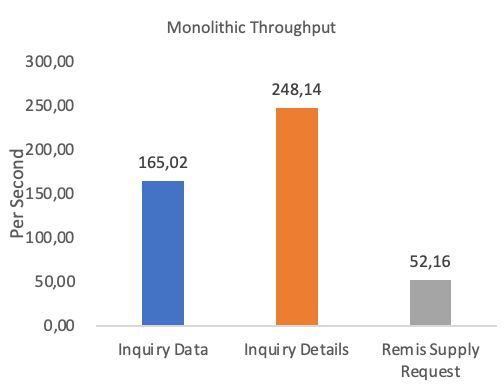
\includegraphics[width=\linewidth]{imagens/maulana_thp_mono.jpg}    
    {\par \raggedright \footnotesize Fonte: \textcite{maulana_design_2022}.\par}
  \end{minipage}%
  \hfill
  \begin{minipage}[t]{0.48\linewidth}
    \caption{Throughput Cenário Microsserviços}
    \label{fig:maulana_thp_ms}
    \centering
    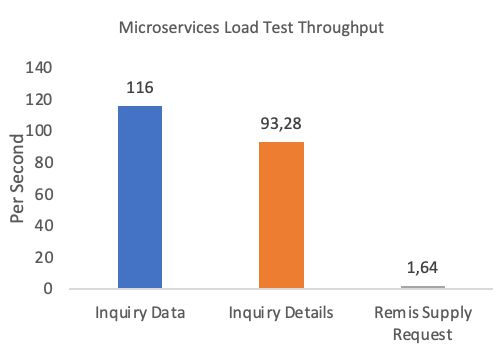
\includegraphics[width=\linewidth]{imagens/maulana_thp_ms.jpg}
    
    {\par \raggedright \footnotesize Fonte: \textcite{maulana_design_2022}.\par}
  \end{minipage}
\end{figure}

Em contraste, nos testes com a arquitetura de microsserviços, os tempos de resposta evidenciam diferenças significativas. O subserviço Remis Supply Request apresenta o maior tempo de resposta médio, de \textbf{4.240,4 ms}, superando consideravelmente o Inquiry Data, que registra \textbf{586 ms}, e o Inquiry Details, que alcança \textbf{552 ms} conforme ilustrado nas figuras \ref{fig:maulana_thp_ms} e \ref{fig:maulana_time_ms}. Os subserviços Inquiry Data e Inquiry Details demonstram resultados instáveis, com variações de desempenho e tendem a diminuir sob alta carga, sugerindo desafios na orquestração e na comunicação entre os novos serviços.

\begin{figure}[htb]
  \centering
  \begin{minipage}[t]{0.48\linewidth}
    \caption{Latência Cenário Monolítico}
    \label{fig:maulana_time_mono}
    \centering
    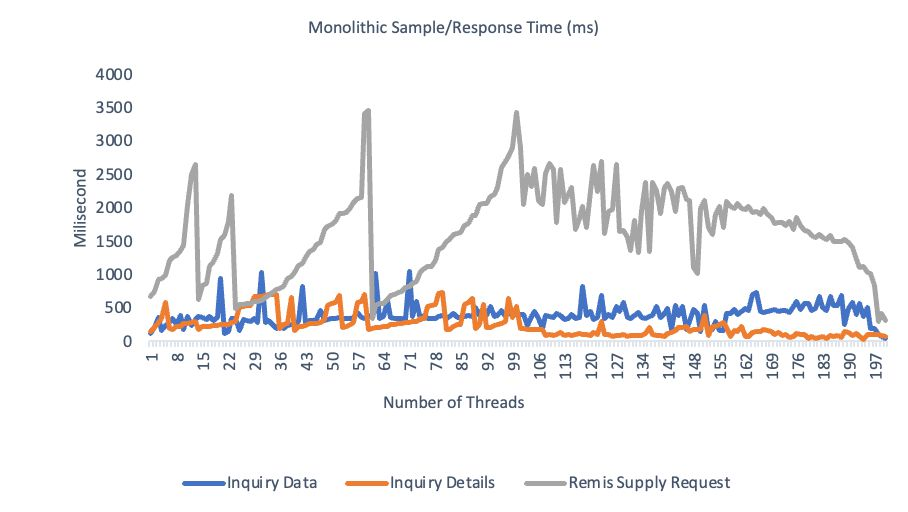
\includegraphics[width=\linewidth]{imagens/maulana_time_mono.jpg}    
    {\par \raggedright \footnotesize Fonte: \textcite{maulana_design_2022}.\par}
  \end{minipage}%
  \hfill
  \begin{minipage}[t]{0.48\linewidth}
    \caption{Latência Cenário Microsserviços}
    \label{fig:maulana_time_ms}
    \centering
    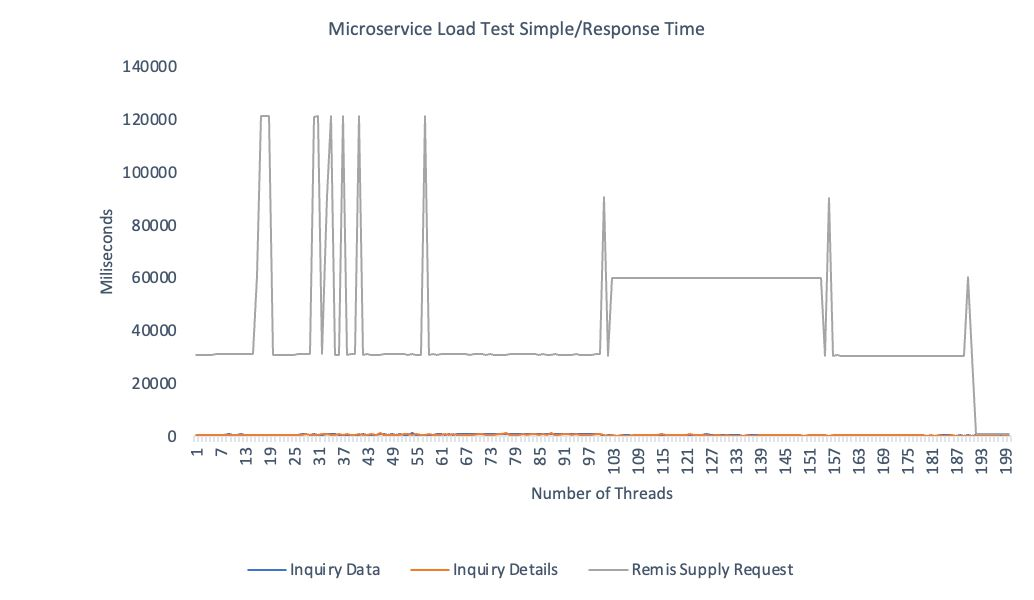
\includegraphics[width=\linewidth]{imagens/maulana_time_ms.jpg}    
    {\par \raggedright \footnotesize Fonte: \textcite{maulana_design_2022}.\par}
  \end{minipage}
\end{figure}

Além dos testes de carga, foram realizados cenários de stress testing para avaliar a capacidade da arquitetura de microsserviços em lidar com grandes volumes de requisições simultâneas. Os autores concluíram que, embora a arquitetura monolítica, executada em servidor on-premises (Intel® Xeon® CPU E5-2680 v3 @ 2.50GHz, 8GB \acrshort{ram} com Docker), tenha apresentado melhor desempenho em alguns testes específicos de tempo de resposta, a arquitetura de microsserviços, hospedada em máquina virtual no Google Compute Engine (n1-standard-2, Intel Haswell 1 vCPU, 7.5GB \acrshort{ram}) com Spring Boot, é preferível para desenvolvimento e manutenção. Isso decorre da simplicidade de gerenciamento, independência entre os subserviços e possibilidade de uso de diferentes tecnologias conforme a necessidade, aspectos inviáveis na arquitetura monolítica \cite{rademacher_modeling_2020}.

 \subsubsection{Resumo do Estudo}

Em síntese, o estudo de \textcite{maulana_design_2022} investigou a migração de um sistema bancário monolítico para microsserviços, com foco nos testes de desempenho em um contexto financeiro real. A pesquisa avaliou métricas como tempo de resposta, latência e \textit{throughput} em cenários de carga e estresse, destacando a capacidade dos microsserviços de atender às demandas de robustez e adaptabilidade do setor bancário. Os resultados indicaram que, embora o desempenho bruto em alguns testes específicos possa favorecer o sistema monolítico, em função das diferentes especificações de hardware utilizadas nos experimentos, a arquitetura de microsserviços é considerada superior para o desenvolvimento e a manutenção, devido à modularidade e à flexibilidade tecnológica. Essas características são cruciais para a agilidade e a inovação exigidas por bancos e outras instituições financeiras.

Contudo, uma limitação significativa do trabalho reside no fato de que os autores não investigaram diferentes formas de orquestração de microsserviços, focando exclusivamente na comparação entre arquiteturas monolítica e de microsserviços. Essa lacuna é particularmente relevante, pois a escolha do protocolo de comunicação entre microsserviços (\gls{rest}, \gls{grpc}, Apache Thrift, entre outros) pode impactar substancialmente o desempenho, a latência e a eficiência operacional do sistema, aspectos críticos para aplicações bancárias que demandam alta disponibilidade e tempos de resposta consistentes. A ausência de uma análise comparativa entre diferentes tecnologias de orquestração constitui uma oportunidade de pesquisa importante para aprofundar a compreensão sobre como otimizar a comunicação inter-serviços em ambientes financeiros distribuídos, reforçando a relevância da presente pesquisa no contexto da transformação digital do setor financeiro.

% -- Jhingran 2024
\subsection{Decentralized Generative AI Model Deployment Using Microservices \cite{jhingran_decentralized_2024}}
\label{subsec:jhingran_decentralized}

\textcite{jhingran_decentralized_2024} propõem uma solução para a implantação de modelos de \acrfull{ia} Generativa de forma descentralizada, utilizando uma arquitetura baseada em microsserviços. O estudo aborda os desafios inerentes à implantação de modelos complexos de \gls{ia} Generativa em sistemas centralizados, como gargalos de desempenho, falta de flexibilidade e dificuldades de escalabilidade. A motivação dos autores reside nas limitações dos sistemas centralizados, que frequentemente resultam em alta latência, comprometimento da integridade dos dados em situações de múltiplas requisições concorrentes \cite{lu_computing_2024}, além do considerável consumo de largura de banda e recursos computacionais. A pesquisa visa demonstrar como a abordagem descentralizada, habilitada por microsserviços, pode otimizar o uso de recursos, melhorar a tolerância a falhas e aumentar a escalabilidade, permitindo a distribuição da carga de trabalho entre múltiplos nós e reduzindo a latência ao processar dados mais próximos da "borda" da rede \cite{jhingran_performance_2021}.

A solução proposta consiste na divisão de modelos de \gls{ia} Generativa em componentes modulares, com cada módulo implementado como um microsserviço \cite{gustrowsky_using_2024}. Esses microsserviços comunicam-se por meio de \acrfull{api}s \gls{rest}, permitindo a execução em ambientes on-premise ou na nuvem. Essa distribuição da carga computacional tem como objetivo reduzir a latência e otimizar a largura de banda. O processo de implantação envolve etapas como o particionamento do modelo em submódulos, a conteinerização (com Docker), a implantação em nós distribuídos (com Kubernetes), o autoescalonamento, o balanceamento de carga, o monitoramento, a tolerância a falhas, a integração \acrfull{ci/cd} e considerações de segurança e privacidade dos dados.

A avaliação do desempenho da solução descentralizada foi realizada por meio de diversas métricas comparativas entre as abordagens centralizada e descentralizada. Os resultados, apresentados na  \autoref{tab:3-jhingran_performance_comparison}, destacam melhorias significativas em áreas como latência, utilização de largura de banda, tolerância a falhas, tempo de resposta, custo, consumo de energia e eficiência na utilização de computação.

\begin{table}[H]
\centering
\caption{Comparação entre Arquiteturas Centralizadas e Descentralizadas.}
\label{tab:3-jhingran_performance_comparison}
\begin{tabularx}{\textwidth}{| X | c | c | c | c |}
\hline
\textbf{Métrica} & \textbf{Monolítica} & \textbf{Microsserviços} & \textbf{Melhoria (\%)} & \textbf{Unidade} \\
\hline
Latência                  & 250ms   & 50ms    & 80 & ms \\
\hline
Uso de Banda              & 100GB   & 30GB    & 70 & GB \\
\hline
Tolerância a Falhas       & 60\%    & 95\%    & 35 & \% \\
\hline
Escalabilidade            & Média   & Alta    & N/A & Qualitativa \\
\hline
Tempo de Resposta         & 500ms   & 100ms   & 80 & ms \\
\hline
Consumo de Energia          & 3000W   & 1200W   & 60 & Watts \\
\hline
Acurácia do Modelo        & 90\%    & 92\%    & 2  & \% \\
\hline
\end{tabularx}
{\par \raggedright \footnotesize Fonte: \textcite{jhingran_decentralized_2024}\par}
\end{table}


A análise dos resultados demonstra claramente as vantagens da implantação dos modelos de \gls{ia} Generativa de forma descentralizada em microsserviços. Esses aspectos são especialmente relevantes para aplicações que exigem eficiência, custo-benefício e confiabilidade. Como pode ser observado na \autoref{tab:3-jhingran_performance_comparison}, a latência foi reduzida em\textbf{ 80\% (de 250 ms para 50ms)} e o tempo de resposta também diminuiu em \textbf{80\% (de 500 ms para 100 ms)}, o que melhora significativamente a experiência do usuário e possibilita processamento em tempo real. Além disso, a utilização da largura de banda apresentou uma melhoria de \textbf{70\%}, indicando menores custos de transferência de dados e maior velocidade no manuseio de informações.

Além disso, a tolerância a falhas aumentou em \textbf{35\%} e a escalabilidade foi classificada como alta, indicando que os sistemas descentralizados são mais resilientes a interrupções e falhas de modelo, o que eleva a confiabilidade e a disponibilidade do sistema. A eficiência de custos é notável, com uma redução de 70\% (de \$5000 para \$1500), o que torna a implantação descentralizada mais econômica para aplicações de \gls{ia} em larga escala. O \textbf{consumo de energia} foi reduzido em\textbf{ 60\%}, alinhando-se aos objetivos de sustentabilidade e diminuindo os custos operacionais. 

\subsubsection{Resumo do Estudo}

O estudo de \textcite{jhingran_decentralized_2024} demonstra experimentalmente as vantagens da implantação descentralizada de modelos de \gls{ia} Generativa em arquiteturas de microsserviços, apresentando melhorias substanciais em \textbf{latência (80\%)}, \textbf{custo (70\%)} e tolerância a \textbf{falhas (35\%)} em comparação com sistemas centralizados. A pesquisa apresenta uma abordagem prática para superar limitações de escalabilidade e recursos em sistemas de \gls{ia}, estabelecendo diretrizes para a implantação distribuída que otimiza o desempenho e a eficiência operacional.

Entretanto, o trabalho apresenta limitações metodológicas importantes que a pesquisa busca endereçar. Enquanto \textcite{jhingran_decentralized_2024} focam em comparações teóricas entre arquiteturas centralizadas e descentralizadas sem especificar protocolos de comunicação ou validação experimental controlada, a investigação preenche essa lacuna ao comparar empiricamente protocolos específicos (\gls{rest}, \gls{grpc}, Apache Thrift) em cenários reais de assistentes virtuais multimodais no setor financeiro. Adicionalmente, a abordagem considera não apenas métricas de desempenho geral, mas também aspectos críticos como latência de cauda (p95, p99) e eficiência de recursos sob diferentes complexidades de processamento de \gls{ia}, oferecendo diretrizes práticas para decisões arquiteturais em domínios de alta criticidade.


\section{Síntese do Capítulo}
\label{sec:sintese_capitulo}

Neste capítulo, foi apresentada uma \acrfull{rsl}, conduzida segundo as diretrizes de \cite{scannavino_revisao_2017}, detalhando bases de dados, estratégias de busca e critérios de seleção para assegurar a qualidade científica dos estudos relacionados à orquestração de microsserviços e \gls{ia} Generativa no setor financeiro.

A análise dos trabalhos revelou três vertentes principais de pesquisa: \textcite{niswar_performance_2024} estabeleceram a superioridade do \gls{grpc} sobre \gls{rest} e \acrshort{graphql} em cenários genéricos, mas sem considerar cargas de \gls{ia} generativa; \textcite{maulana_design_2022} demonstraram a viabilidade da migração para microsserviços no setor bancário, porém sem especificar protocolos de comunicação ou métricas de latência de cauda; e \textcite{jhingran_decentralized_2024} propuseram vantagens teóricas da descentralização em \gls{ia} generativa, mas sem validação experimental controlada.

Esta pesquisa preenche lacunas identificadas ao combinar aspectos dos três trabalhos: a comparação rigorosa de protocolos de comunicação (expandindo para incluir Apache Thrift), o foco específico no setor financeiro (com requisitos de latência críticos), e a aplicação prática em sistemas de \gls{ia} generativa multimodal (validada experimentalmente). A contribuição, conforme comparada na \autoref{tab:posicionamento_estado_arte}, se posiciona como a primeira investigação experimental abrangente sobre orquestração de microsserviços para assistentes virtuais multimodais no contexto financeiro, oferecendo diretrizes práticas baseadas em evidências empíricas para decisões arquiteturais em um domínio de alta criticidade.

\begin{table}[htbp]
\centering
\caption{Posicionamento deste trabalho no Estado da Arte}
\label{tab:posicionamento_estado_arte}
\makebox[\textwidth]{%
\begin{tabularx}{1.2\textwidth}{|l|X|X|X|X|}
\hline
\textbf{Aspecto} & \textbf{\textcite{niswar_performance_2024}} & \textbf{\textcite{maulana_design_2022}} & \textbf{\textcite{jhingran_decentralized_2024}} & \textbf{Esta Dissertação} \\
\hline
Domínio de Aplicação & Sistema Educacional & Sistema Bancário Genérico & \gls{ia} Generativa Genérica & \textbf{Assistentes Virtuais Financeiros Multimodais} \\
\hline
Protocolos Comparados & \gls{rest}, \acrshort{graphql}, \gls{grpc} & Monolítico vs Microsserviços & Centralizado vs Descentralizado & \textbf{\gls{rest}, \gls{grpc}, Apache Thrift} \\
\hline
Ambiente de Teste & Dados estáticos & Migração real limitada & Teórico/simulado & \textbf{Ambiente controlado com \gls{ia} real} \\
\hline
Métricas de Latência & Tempo médio de resposta & Tempo de resposta básico & Comparação teórica & \textbf{p50, p95, p99 + máximos} \\
\hline
Complexidade dos Cenários & Dados planos vs aninhados & Carga única & Não especificado & \textbf{Simples, Tradicional, Complexo} \\
\hline
Foco em \gls{ia} Generativa & Não & Não & Sim (Teórico) & \textbf{Sim (Experimental)} \\
\hline
Setor Financeiro & Não & Sim (Genérico) & Não & \textbf{Sim (Específico)} \\
\hline
Tamanho Amostral & Limitado & Caso único & N/A & \textbf{15 replicações × 3 cenários × 3 protocolos} \\
\hline
Multimodalidade & Não & Não & Sim (\gls{llm}) & \textbf{Sim (\gls{stt}, \gls{llm} e \gls{tts})} \\
\hline
\end{tabularx}%
}
{\par \raggedright \footnotesize Fonte: Elaborado pelo autor.\par}
\end{table}


\chapter{Metodologia}
\label{ch:4metodologia}

\section{Classificação da pesquisa}

Este trabalho adota uma abordagem metodológica \textbf{mista}, combinando uma revisão sistemática da literatura com uma análise experimental controlada. Trata-se de um estudo de natureza \textbf{aplicada}, no qual diferentes protocolos de comunicação entre microsserviços são avaliados empiricamente. Os objetivos do estudo demandam a medição objetiva de desempenho (latência, vazão, uso de recursos, etc.) sob cada protocolo, o que justifica a escolha por um delineamento experimental. Alternativas como análises puramente teóricas ou simulações não seriam adequadas para capturar todas as nuances de desempenho em um ambiente real. Por isso, optou-se por implementar um cenário de teste concreto e coletar métricas diretamente, permitindo a quantificação das diferenças de performance e uso de recursos além da verificação da superioridade de algum protocolo em termos práticos. Além disso, por meio de comparações estatísticas, busca-se verificar se eventuais diferenças observadas são estatisticamente significativas e relevantes.

No contexto deste trabalho, realizou-se uma série de testes de uso em uma aplicação distribuída em microsserviços de um protótipo de assistente virtual multimodal com \acrfull{ia} generativa, utilizando exemplos do setor financeiro como cenários. Em suma, a metodologia foi planejada para garantir validade interna, controlando variáveis relevantes, produzindo dados quantitativos confiáveis e possibilitando a comparação direta entre as três abordagens de comunicação.

\section{Etapas da pesquisa}
Esta pesquisa pode ser divida em 4 etapas:

\begin{itemize}
    \item \textbf{Revisão bibliográfica}: Esta etapa consistiu em um estudo aprofundado das principais tecnologias de microsserviços e orquestração, detalhada no \autoref{ch:2pilares} e no \autoref{ch:3estado_da_arte}. O objetivo foi estabelecer uma base teórica sólida e, ao mesmo tempo, buscar por análises comparativas similares, garantindo a originalidade e a relevância da pesquisa.
    
    \item \textbf{Desenvolvimento da arquitetura de testes}: Nesta fase, descrita na \autoref{sec:4-arquitetura_testes}, o objetivo foi projetar e implementar a arquitetura de microsserviços do assistente virtual. Isso incluiu o desenvolvimento dos serviços individuais (\acrshort{stt}, \acrshort{llm}, \acrshort{tts}), a definição das interfaces de comunicação e a configuração de um ambiente de teste controlado para garantir a fidelidade do experimento.
    
    \item \textbf{Experimentos}: Esta etapa foi a execução prática dos testes, detalhada na \autoref{sec:4-procedimentos_experimentais}. Nela, o sistema foi submetido a diferentes cenários de demanda (simples, tradicional e complexa) para coletar dados quantitativos sobre o comportamento de cada protocolo de comunicação sob variadas condições de estresse.
    
    \item \textbf{Análise de dados}: O objetivo final foi processar e interpretar os dados brutos coletados durante os experimentos, conforme apresentado no \autoref{ch:5resultados}. As métricas de desempenho e uso de recursos foram analisadas para extrair \textit{insights} significativos, identificar padrões e, finalmente, formular as conclusões do estudo.
\end{itemize}



\section{Arquitetura de testes}
\label{sec:4-arquitetura_testes}

O experimento foi elaborado com base em uma arquitetura de microsserviços representativa de um assistente virtual multimodal com \acrfull{ia} generativa. A \autoref{fig:4-arquitetura-experimentos} ilustra a arquitetura proposta, a qual consiste em um serviço orquestrador (\textit{gateway} do assistente) que recebe as requisições dos usuários e coordena chamadas para serviços especializados de \textit{backend}. Cada teste isolou um protocolo de comunicação de cada vez (\gls{rest}, \gls{grpc} ou Thrift) para permitir uma comparação justa dos resultados. Esse delineamento possibilitou identificar o impacto do mecanismo de orquestração na performance do sistema, alinhando-se aos objetivos de determinar qual tecnologia oferece menor latência e maior eficiência. 

\begin{figure}[H]
\caption{Arquitetura de microsserviços do assistente virtual multimodal}
\label{fig:4-arquitetura-experimentos}
\centering
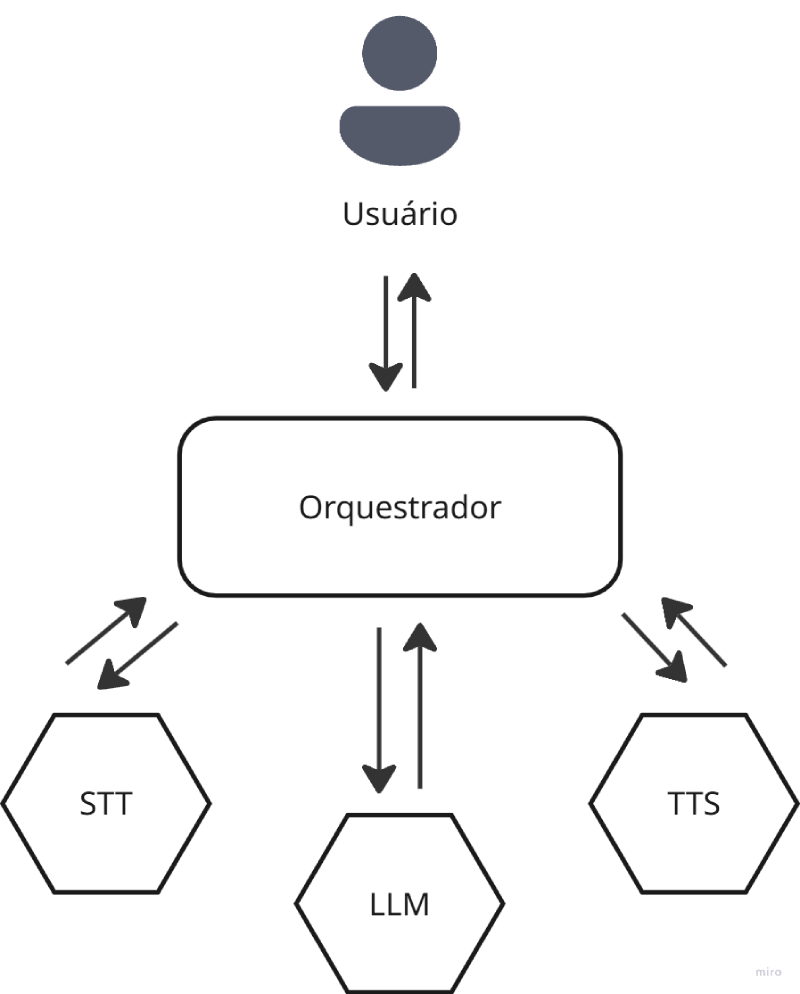
\includegraphics[width=0.4\textwidth]{imagens/4-arquitetura_cenario.png}
{\par \raggedright \footnotesize Fonte: Elaborado pelo autor.}
\end{figure}

Com arquivos de áudios pré-definidos, simularam-se cenários de interação por voz (Detalhado em \ref{sec:4-procedimentos_experimentais}), onde o orquestrador aciona um microserviço de reconhecimento de fala (\acrshort{stt}) que converte áudio em texto e, em seguida, encaminha esse texto ao serviço de \gls{ia} generativa (\acrshort{llm}). A resposta textual pode ser, posteriormente, enviada a um microserviço de síntese de voz (\acrshort{tts}) que retorna áudio ao usuário. Todos esses serviços (\acrshort{stt}, \acrshort{llm}, \acrshort{tts}) são implementados como microsserviços independentes que se comunicam por meio de rede. Essa divisão reflete cenários reais de assistentes multimodais, nos quais diferentes módulos gerenciam modalidades distintas de dados (texto, voz e imagem) em um fluxo de processamento.

Para fins do experimento, a arquitetura acima foi implantada em três configurações distintas, variando apenas o protocolo de comunicação utilizado nas chamadas remotas:

\begin{itemize}
\item \textbf{Configuração \gls{rest}}: todos os microsserviços expõem \gls{api}s \gls{rest} (\acrshort{http}/1.1 com \acrshort{json}). O serviço orquestrador invoca os demais via chamadas \acrshort{http} \gls{rest} tradicionais (endpoints RESTful).
\item \textbf{Configuração \gls{grpc}}: os microsserviços utilizam \gls{grpc} sobre \acrshort{http}/2, com interfaces definidas em arquivos \texttt{.proto} e dados serializados em \textit{Protocolo Buffers}. O orquestrador atua como cliente \gls{grpc} para os outros serviços, usando esquemas gerados a partir dos \texttt{.proto}.
\item \textbf{Configuração Thrift}: os microsserviços comunicam-se via Apache Thrift, utilizando uma interface Thrift comum. O orquestrador chama os serviços através dos clientes Thrift gerados.
\end{itemize}

Em cada configuração, a lógica de negócio dos microsserviços permanece idêntica, assim como os dados trocados e a sequência de chamadas no pipeline do assistente. Dessa forma, isola-se o impacto do protocolo de comunicação, garantindo que quaisquer diferenças de desempenho sejam atribuídas, principalmente, ao \textit{overhead} de comunicação (formato de serialização, transporte etc.) e não à funcionalidade em si. Cada protocolo foi avaliado separadamente, iniciando o experimento com \gls{rest}, seguido pela repetição com \gls{grpc} e, por fim, com Thrift.

É importante ressaltar que, para possibilitar a troca do protocolo de forma transparente, foram desenvolvidas adaptações ou interfaces duplas quando necessário. Definiram-se modelos de dados equivalentes em \acrshort{json}, mensagens \textit{Protocol} Buffers e \textit{structs} Thrift, assegurando a mesma uniformidade de conteúdo e o tamanho do \textit{payload} em cada cenário. Isso garantiu a comparabilidade direta. Durante cada execução, apenas um protocolo permaneceu ativo, prevenindo interferências mútuas. Assim, obtêm-se medidas repetidas para cada protocolo, permitindo análises emparelhadas e redução de variabilidade.

\subsubsection{Justificativa da Seleção de Protocolos}
\label{subsec:justificativa-protocolos}

A seleção dos protocolos \acrshort{rest}, \acrshort{grpc} e Apache Thrift para esta pesquisa foi fundamentada em critérios que buscam abranger os paradigmas de comunicação mais relevantes e adotados na indústria para orquestração de microsserviços, conforme comparado anteriomente na \autoref{tab:2-protocolos}.

O protocolo \acrshort{rest} foi incluído por representar o padrão \textit{de facto} e amplamente consolidado para APIs web. Sua ubiquidade, simplicidade de implementação e interoperabilidade o tornam uma base obrigatória para qualquer análise comparativa, servindo como \textit{baseline} para mensurar ganhos de performance de alternativas mais modernas.

Os protocolos \acrshort{grpc} e Apache Thrift foram selecionados por representarem o estado da arte em comunicação binária eficiente. Ambos utilizam serialização binária (\textit{Protocol Buffers} e formato binário próprio, respectivamente) e operam sobre protocolos de transporte modernos (\acrshort{http}/2 e \acrshort{tcp}), sendo projetados especificamente para oferecer alta performance e baixa latência em ambientes de sistemas distribuídos. Sua inclusão permite avaliar o trade-off entre a simplicidade do \acrshort{rest} e a eficiência de soluções orientadas a performance.

Optou-se por não incluir tecnologias como \acrshort{graphql} ou Apache Kafka no escopo experimental deste estudo. Ambas as soluções, embora relevantes em contextos específicos, introduziriam variáveis arquiteturais que comprometeriam a equivalência direta desejada para esta análise comparativa. O \acrshort{graphql} normalmente requer um gateway ou camada de agregação, introduzindo um componente intermediário não presente na comunicação ponto a ponto avaliada nos demais protocolos. O Kafka atua primordialmente em paradigmas assíncronos de mensageria, enquanto o foco desta pesquisa reside estritamente na comunicação síncrona entre microsserviços em um pipeline de IA multimodal, cujos contratos são fixos e conhecidos. Essa escolha por protocolos de comunicação direta e síncrona possibilitou a manutenção da equivalência arquitetural entre os cenários testados, isolando o impacto do protocolo de comunicação como variável principal.

Portanto, a tríade \acrshort{rest}-\acrshort{grpc}-Thrift forma um conjunto representativo e tecnicamente contrastante, permitindo uma análise abrangente entre o padrão textual ubíquo (\acrshort{rest}) e as principais alternativas binárias de alto desempenho (\acrshort{grpc} e Thrift).

\subsection{Ambiente de Teste}

Os experimentos ocorreram em um ambiente de teste controlado, configurado em uma nuvem privada, com o intuito de replicar condições realistas de produção e isolar fatores externos, como flutuações na rede, processos agendados do sistema operacional e interferência de outras aplicações. Dessa forma, toda a infraestrutura foi configurada utilizando \textbf{contêineres Docker}, o que representa um ambiente típico de microsserviços em escala. Essa escolha possibilita a reprodução do experimento e assegura que cada modelo seja executado em um contêiner isolado, com controle sobre alocações de CPU e memória, evitando interferências.

Em termos de hardware, utilizou-se um servidor dedicado com  capacidade suficiente para executar modelos de \gls{ia} que integram os microsserviços, como \acrshort{stt}, \acrshort{llm} e \acrshort{tts}, conforme detalhado na \autoref{tab:4-especificacoes-hardware}. 

\begin{table}[H]
\centering
\caption{Especificações do hardware utilizado nos experimentos}
\label{tab:4-especificacoes-hardware}
\begin{tabularx}{\linewidth}{|l|X|}
\hline
\textbf{Componente} & \textbf{Especificação} \\
\hline
Processadores (CPU) & Processador Intel Xeon Platinum 8273CL @ 2.20GHz (turbo 2.9 GHz); 12 núcleos/24 threads por soquete; \\
\hline
Memória \acrshort{ram} & 85GB disponíveis; \textit{sem swap}. \\
\hline
Armazenamento & Sistema: 200GB; Dados: NVMe 2TB. \\
\hline
Placa Gráfica (\acrshort{gpu}) & NVIDIA Tesla A100 de 40 GB \\
\hline
Sistema Operacional & Oracle Linux Server 9.6 (\texttt{platform:el9}); arquitetura x86\_64 \\
\hline
Referência GCP & a2-highgpu-1g \\
\hline
\end{tabularx}
{\par \raggedright \footnotesize Fonte: Elaborado pelo autor.\par}
\end{table}

\subsubsection{Justificativa do Ambiente de Alto Desempenho}
\label{subsec:justificativa-hardware}

Os experimentos foram conduzidos em um ambiente de alto desempenho, conforme detalhado na \autoref{tab:4-especificacoes-hardware}. Esta escolha foi intencional e estrategicamente alinhada ao objetivo central do estudo: isolar e avaliar o impacto dos protocolos de comunicação na orquestração de microsserviços, minimizando interferências relacionadas a limitações de hardware no processamento de modelos de IA.

Em testes preliminares realizados em ambientes com recursos computacionais modestos, observou-se que a carga inerente ao processamento de modelos de IA generativa, especialmente modelos grandes como Whisper e LLMs, consumia a maior parte dos recursos de CPU e , configurando-se como um gargalo dominante. Nessas condições, as diferenças de desempenho entre os protocolos de comunicação tornaram-se marginalmente perceptíveis, uma vez que a latência foi majoritariamente determinada pelo tempo de inferência dos modelos e não pela eficiência da comunicação entre os serviços.

Ao utilizar um hardware compatível, assegurou-se que os modelos de IA operassem dentro de patamares de latência previsíveis, além de garantir recursos suficientes para lidar com a carga de processamento multimodal. Dessa forma, o impacto relativo da comunicação entre microsserviços pôde ser amplificado e observado de maneira mais clara e isolada, atendendo ao propósito comparativo do estudo.

O foco nesta fase foi avaliar o comportamento dos protocolos em condições ideais de processamento, estabelecendo um \textit{baseline} de desempenho livre de ruídos causados pela escassez de recursos. Estudos futuros poderão investigar o comportamento desses protocolos em ambientes com restrições de hardware ou em arquiteturas híbridas, expandindo a aplicabilidade das conclusões.

\section{Procedimentos Experimentais}
\label{sec:4-procedimentos_experimentais}

Nesta seção são descritos os procedimentos experimentais em detalhe, incluindo o planejamento das execuções, geração de cenário e coleta de dados. O experimento seguiu um protocolo padronizado para cada configuração de teste (\gls{rest}, \gls{grpc}, Thrift), variando apenas o protocolo em uso.

\subsection{\textit{Workloads} e Cenários de Teste}

Todos os cenários de demanda definidos para este experimento simulam interações via \textbf{entrada de voz}, variando apenas o nível de complexidade cognitiva da solicitação feita ao assistente virtual. Em cada caso, a entrada de voz é processada pelo pipeline completo de microsserviços: \acrfull{stt}, processamento de linguagem natural e raciocínio por \acrfull{llm}, e, por fim,  \acrfull{tts} para entrega da resposta.

Foram definidos três cenários:

\begin{itemize}
    \item \textbf{Cenário 1 (simples)}: Solicitação objetiva e direta, que requer apenas uma busca simples de informação factual. Para este cenário, não injetamos nenhum contexto extra. \\
    Áudio: "Qual é o código do ativo da Petrobras?" \\
    Esse cenário envolve processamento mínimo no \gls{llm}, com baixa demanda de inferência e retorno rápido.
    \item \textbf{Cenário 2 (tradicional)}: Pergunta de dificuldade intermediária, que exige interpretação conceitual e comparação entre dois elementos do domínio financeiro. Para este cenário, injetamos o contexto de um manual do investidor, como o disponibilizado pela CVM\footnote{Disponível em: \url{https://www.gov.br/investidor/pt-br/educacional/programa-bem-estar-financeiro/programa-bem-estar-financeiro-arquivos/apostila-06.pdf}. Acesso em: 26 jul. 2025.}. \\
    Áudio: "Qual a diferença entre renda fixa e Ibovespa?" \\
    Esse cenário requer raciocínio moderado no \gls{llm}, incluindo compreensão de conceitos e elaboração de resposta explicativa.
    \item \textbf{Cenário 3 (complexo)}: Consulta complexa que demanda análise de dados históricos e síntese de informações. Para este cenário, fornecemos um contexto com dados diários das ações de 2024 em formato \gls{csv}, simulando a consulta a uma fonte interna de informações de mercado. \\
    Áudio: "Quais foram as melhores ações de 2024?" \\
    Esse cenário impõe maior tempo de raciocínio ao \gls{llm}, podendo envolver consultas a fontes internas, ordenação e seleção de dados para compor a resposta.
\end{itemize}

A justificativa para os cenários propostos está em simular o comportamento de um aplicativo de informações e análise para investidores, um público-alvo que hoje representa 59 milhões de investidores individuais na B3 \cite{anbima_raio_nodate}. A diversidade de usuários e a natureza de suas interações diárias foram a base para a concepção dos três níveis de demanda. O Cenário Simples reflete o comportamento de investidores iniciantes, que buscam informações simples para aprender sobre o mercado. O Cenário Tradicional representa o investidor tradicional, com dúvidas cotidianas e a necessidade de comparar conceitos e ativos. Já o Cenário Complexo simula o usuário mais experiente, que busca extrair informações úteis e realizar análises aprofundadas para tomar decisões de investimento, impondo uma carga de processamento significativamente maior ao sistema. Deste modo, os cenários foram desenhados para representar o comportamento agregado de uma carteira de clientes, e não de um único usuário, validando a abordagem em um contexto de aplicação real e em escala.

Em todos os cenários, o fluxo de processamento é idêntico: o áudio da pergunta é enviado ao serviço de \gls{stt}, convertido em texto, processado pelo \gls{llm} para gerar a resposta textual e, finalmente, sintetizado em áudio pelo serviço de \gls{tts}. A variação no tempo de resposta e no consumo de recursos ocorre principalmente em função da complexidade do raciocínio exigido em cada cenário, permitindo avaliar o impacto do protocolo de comunicação em diferentes níveis de carga cognitiva.

\subsection{Execução dos Testes}

Para a execução dos cenários de testes, utilizou-se uma combinação de duas ferramentas: k6\footnote{Disponível em \url{https://k6.io}} para a geração de carga e coleta de métricas do lado do cliente, e Prometheus\footnote{Disponível em \url{https://prometheus.io}} para o monitoramento de recursos do lado do servidor. Com o k6, foram desenvolvidos scripts em JavaScript para simular o comportamento dos usuários em cada um dos cenários definidos (simples, tradicional e complexo). Esses scripts foram configurados para realizar chamadas ao endpoint do serviço orquestrador, enviando os áudios pré-definidos e medindo as métricas de resultado, como latência (p50, p95, p99), throughput e taxas de erro. Em paralelo, o ambiente foi instrumentado com o Prometheus para coletar, em tempo real, as métricas de desempenho da infraestrutura. Por meio de exporters configurados nos contêineres, o Prometheus monitorou o uso de CPU e memória de cada microsserviço, fornecendo uma visão detalhada do consumo de recursos sob estresse.

Cada configuração de protocolo (\gls{rest}, \gls{grpc} e Thrift) foi submetida ao mesmo rigor de testes, com 15 replicações independentes por protocolo para garantir um tamanho amostral estatisticamente relevante. Entre a avaliação de cada protocolo, o sistema era reiniciado para limpar completamente o estado e evitar interferências entre os testes. A ordem de execução dos cenários foi randomizada para todos os protocolos, o que evitou viés e assegurou que a única variável entre os experimentos fosse a tecnologia de comunicação, permitindo uma comparação direta e justa dos resultados.

Durante todos os experimentos, o ambiente foi monitorado para identificar anomalias ou interferências externas, como picos de CPU na máquina host ou atividades de rede não relacionadas ao teste, garantindo que nenhuma condição externa contaminasse os resultados. Não foi necessário descartar nenhuma execução por comportamento anômalo. Ao final dos procedimentos, obteve-se um conjunto robusto de dados brutos, incluindo tempos de resposta de milhares de requisições e a utilização de recursos por microsserviço, que foram agregados e analisados nas seções subsequentes.

\section{Métricas e Variáveis de Avaliação}
\label{sec:5-metricas-variaveis}

Foram definidas algumas \textbf{métricas de desempenho} para avaliar quantitativamente cada protocolo. As métricas escolhidas contemplam aspectos de latência de resposta (incluindo cauda), capacidade de throughput, eficiência de recursos e confiabilidade. A \textbf{\autoref{tab:4-metricas}} resume as principais métricas coletadas e suas definições.

\begin{table}[H]
\centering
\caption{Métricas coletadas nos experimentos e sua descrição.}
\label{tab:4-metricas}
\begin{tabularx}{\linewidth}{|p{4cm}|X|}
\hline
\textbf{Métrica} & \textbf{Descrição} \\
\hline
\textit{Latência (p50, p95, p99)} & Tempo de resposta end-to-end, em milissegundos (ms), desde a chegada da requisição ao orquestrador até o envio completo da resposta ao cliente. Reporta-se a mediana (p50) e as latências de cauda (p95 e p99), fundamentais em contextos financeiros por evidenciarem picos que podem impactar a experiência do usuário e operações sensíveis. \\
\hline
\textit{Vazão} (Throughput) & Número de requisições processadas por segundo pelo sistema. Mede a capacidade de atendimento sob carga, normalmente expresso em req/s. \\
\hline
\textit{Uso de CPU} & Porcentagem de utilização do(s) CPU(s) pelos microsserviços durante o teste. Medido como média de CPU time total consumido. Indica a eficiência computacional do protocolo. \\
\hline
\textit{Uso de Memória} & Quantidade de memória \acrshort{ram} ocupada pelos serviços durante a execução. Ajuda a identificar \textit{overhead} de alocação de memória de cada framework. \\
\hline
\textit{Taxa de Erro} & Porcentagem de requisições que resultaram em erro (código \acrshort{http} \$\ge\$ 400 ou exceções nas chamadas \gls{rpc}) ou \textit{timeout}. Mede a confiabilidade sob estresse. Espera-se taxas de erro baixas (idealmente 0\%). \\
\hline
\end{tabularx}
{\par \raggedright \footnotesize Fonte: Elaborado pelo autor.\par}
\end{table}

Essas métricas foram escolhidas para cobrir tanto a perspectiva do usuário final (latência, taxa de erro) que afetam diretamente a qualidade do serviço percebida, quanto a perspectiva do provedor do serviço (throughput, uso de CPU/memória) que afetam escalabilidade e custo. Em alinhamento com trabalhos correlatos e diretrizes de avaliação de \gls{api}s, focou-se especialmente em \textbf{tempos de resposta e throughput}, bem como em métricas de \textbf{uso de recursos}. Em particular, a análise de \textbf{latência de cauda (p95 e p99)} fornece uma visão mais realista do comportamento sob pico do que medidas de tendência central isoladas.

A latência medida \textit{end-to-end} foi computada para cada requisição individual. Os percentis \textit{p50}, \textit{p95} e \textit{p99} foram calculados a partir do conjunto dessas observações por cenário e replicação. O \textit{throughput} foi inferido tanto pelo lado do cliente (número total de requisições concluídas dividido pelo tempo de teste) quanto monitorado no lado servidor (contadores de requisições por segundo). As métricas de \textit{uso de CPU e memória} foram coletadas via Prometheus a cada intervalo de 5 segundos durante os testes. A \textit{taxa de erro} foi medida pelo gerador de carga: qualquer resposta inválida ou ausência de resposta dentro de um tempo limite de 6 segundos (\textit{timeout}) foi contabilizada como erro.

Todas as métricas foram registradas para cada replicação de teste, permitindo agregações simples e comparações diretas entre protocolos. Para latência, reportam-se explicitamente \textit{p50}, \textit{p95} e \textit{p99}; quando necessário para sumarização entre replicações, utiliza-se a média desses percentis por cenário.

\subsection{Variáveis, fatores e métricas}
\label{sec:4-variaveis}

Abaixo estão listadas as variáveis, fatores e métricas analisadas em cada cenário.

\subsubsection*{Variáveis de cenário}
\begin{itemize}
\item \textbf{Protocolo} : {\gls{rest}, \gls{grpc}, Thrift}.
\item \textbf{Cenário de uso} : {simples, tradicional e complexo}.
\end{itemize}

\subsubsection*{Variáveis dependentes (métricas de resultado)}
\begin{itemize}
\item \textbf{Latência end-to-end} (ms): p50, p95, p99 e \textbf{máximo} (k6).
\item \textbf{Vazão} média (req/s).
\item \textbf{Uso de CPU} (média) agregado (cAdvisor/Prometheus).
\item \textbf{Uso de memória} (média) agregado (cAdvisor/Prometheus).
\end{itemize}

\subsubsection*{Variáveis controladas}
\begin{itemize}
\item \textbf{Infraestrutura}: hardware único, \acrshort{so}, kernel, rede local e \textit{runtime} de contêineres fixos.
\item \textbf{Nível de Carga} : {1000 usuários virtuais simultâneos}.
\item \textbf{Versões}: imagens, bibliotecas, serializações (\acrshort{json}/Protobuf/Thrift) e configurações.
\item \textbf{Condições de execução}: \textit{warm-up}, número de repetições, ordem randomizada.
\end{itemize}

\subsection{Critérios de Comparação}

Os resultados obtidos para cada protocolo nos três cenários de carga (simples, tradicional e complexo) foram agregados por meio de estatísticas descritivas. Para \textbf{throughput}, \textbf{utilização de CPU}, \textbf{utilização de memória} e \textbf{taxa de erro}, adotou-se a \textbf{média aritmética} por cenário e protocolo. Para \textbf{latência}, a comparação considera explicitamente os percentis \textbf{p50}, \textbf{p95} e \textbf{p99}; quando necessário, emprega-se a média desses percentis entre as replicações de cada cenário.

A avaliação é \textbf{descritiva e visual}, utilizando tabelas e gráficos (incluindo barras) para \textit{p50}, \textit{p95} e \textit{p99}, além das demais métricas, permitindo a inspeção direta das diferenças de desempenho entre os protocolos.

A interpretação dos resultados ocorre pela observação conjunta das métricas. Em ambientes financeiros, prioriza-se \textbf{redução de cauda} (menores \textit{p95} e \textit{p99}) sem degradação relevante do \textit{p50}, aliada a maior eficiência de recursos (menor consumo médio de CPU/memória) e \textbf{baixa taxa de erro}. Dessa forma, identifica-se, para cada nível de demanda, qual protocolo apresenta comportamento mais consistente e previsível, condição essencial para transações sensíveis e \acrshort{sla}s rigorosos.

\section{Ambiente de Teste e Metodologia Experimental}
\label{sec:ambiente_teste}

\subsection{Repositório GitHub com Implementação Completa}
\label{subsec:repositorio_github}

Todo o ambiente de teste, scripts de configuração, implementações dos protocolos e scripts de coleta de dados estão disponíveis publicamente no repositório GitHub do projeto. Este material completo permite a reprodução exata dos experimentos realizados e serve como base para futuros trabalhos na área. O repositório pode ser acessado em:

\begin{center}
\url{https://github.com/luizjr8/mpes-lssj-analise-orquestracao-microsservicos/}
\end{center}

O repositório contém:

\begin{itemize}
\item \textbf{Configurações de ambiente}: Dockerfiles e scripts de provisionamento
\item \textbf{Implementações dos protocolos}: Código fonte para \acrshort{rest}, \acrshort{grpc} e Thrift (em branches separadas)
\item \textbf{Scripts de teste}: Conjunto completo de testes de carga e desempenho
\item \textbf{Dados brutos}: Resultados coletados durante os experimentos
\item \textbf{Relatórios}: Script python (Jupyter Notebook) com a geração das médias, valores e gráficos.
\end{itemize}

\subsection{Diagrama de Fluxo do Processo Experimental}
\label{subsec:diagrama_fluxo}

A metodologia experimental seguida neste trabalho segue um fluxo sistemático e reproduzível, conforme ilustrado na Figura \ref{fig:4-fluxo-experimentos}. Esse modelo estruturado de testes constitui uma das contribuições significativas deste estudo, proporcionando um framework abrangente para a avaliação comparativa de protocolos de comunicação em ambientes de microsserviços.

\begin{figure}[H]
\caption{Fluxo das etapas dos experimentos: da preparação do ambiente à análise e reporte dos resultados, com loops por cenários e protocolos e repositório público para reprodutibilidade.}
\label{fig:4-fluxo-experimentos}
\centering
\begin{tikzpicture}[
  node distance=8mm,
  font=\footnotesize,
  proc/.style={rectangle, rounded corners, draw=black, very thick, fill=gray!12,
               minimum width=10.5cm, align=center, inner sep=6pt},
  loop/.style={proc, dashed},
  arrow/.style={-Latex, thick}
]

\node[proc] (setup) {Preparação do ambiente de testes\\
(Docker Compose, Prometheus+cAdvisor, k6)};
\node[loop, below=of setup] (cenarios) {Loop de \textbf{cenários de carga}\\
(leve, médio, pesado)};
\node[loop, below=of cenarios] (protocolos) {Loop de \textbf{protocolos}\\
(\acrshort{rest}, \acrshort{grpc}, Thrift)};
\node[proc, below=of protocolos] (execute) {Executar teste (warm-up, repetições, ordem randomizada)};
\node[proc, below=of execute] (coletar) {Coletar métricas (k6/Prometheus):\\
latência (p50/p95/p99/máx), throughput, CPU, RAM};
\node[proc, below=of coletar] (persistir) {Persistir artefatos: \texttt{summary.json}, séries \gls{csv}, \textit{logs}};
\node[proc, below=of persistir] (analizar) {Agregação e análise comparativa\\
(médias, p95/p99, $\Delta\%$ vs.\ baseline)};
\node[proc, below=of analizar] (relatorios) {Geração de tabelas e gráficos para o Cap.~\ref{ch:5resultados}};

% seta principal
\draw[arrow] (setup) -- (cenarios);
\draw[arrow] (cenarios) -- (protocolos);
\draw[arrow] (protocolos) -- (execute);
\draw[arrow] (execute) -- (coletar);
\draw[arrow] (coletar) -- (persistir);
\draw[arrow] (persistir) -- (analizar);
\draw[arrow] (analizar) -- (relatorios);

% --- LOOP externo: persist -> (direita) -> (sobe com seta) -> topo do bloco de cenários
\coordinate (loopR)   at ([xshift=20mm]persistir.east);        % ponto à direita do 'persist'
\coordinate (loopTop) at ([xshift=20mm]cenarios.east); % ponto alinhado ao topo dos cenários

\draw[dashed, thick]           (persistir.east) -- (loopR);     % horizontal (sem seta)
\draw[dashed, thick]   (loopR) -- (loopTop);          % vertical para cima (com seta na ponta)
\draw[-Latex, dashed, thick]           (loopTop) -- (cenarios.east); % horizontal de volta ao topo dos cenários

\end{tikzpicture}
{\par \raggedright \footnotesize Fonte: Elaborado pelo autor.\par}
\end{figure}

O processo experimental, detalhado no diagrama, compreende as seguintes etapas principais:

\begin{enumerate}
\item \textbf{Preparação do Ambiente}: Configuração da infraestrutura containerizada com Docker
\item \textbf{Implementação dos Protocolos}: Desenvolvimento das interfaces para cada tecnologia
\item \textbf{Instrumentação}: Configuração de ferramentas de monitoramento (Prometheus, cAdvisor)
\item \textbf{Execução dos Testes}: Aplicação sistemática das cargas de trabalho definidas
\item \textbf{Coleta de Dados}: Captura automatizada das métricas de desempenho
\item \textbf{Análise e Consolidação}: Processamento estatístico dos resultados obtidos
\end{enumerate}

Este modelo de teste não apenas garante a confiabilidade dos resultados apresentados, mas também estabelece um padrão replicável para avaliação de tecnologias de comunicação em arquiteturas de microsserviços, representando uma contribuição prática significativa para a comunidade de engenharia de software.




\chapter{Análise dos Resultados}
\label{ch:5resultados}

Este capítulo apresenta os resultados obtidos durante a execução dos experimentos comparativos entre os protocolos de comunicação \gls{rest}, \gls{grpc}~e Apache Thrift em um ambiente de microsserviços para assistentes virtuais multimodais no contexto financeiro. Foram conduzidos testes nos três cenários definidos no \autoref{ch:4metodologia}: Simples, Tradicional e Complexo, cada um submetido a uma carga constante de 1.000 usuários simultâneos. Para cada combinação de cenário e protocolo, foram coletadas \textbf{15 amostras}, totalizando \textbf{135 execuções}. 

A análise é realizada a partir de duas perspectivas principais: (1) a do cliente, utilizando métricas de latência (avg, max, p90, p95) e throughput coletadas pela ferramenta k6; e (2) do servidor, com métricas de uso de CPU e memória coletadas via Prometheus. Para validar estatisticamente as diferenças de desempenho observadas entre os protocolos e cenários, foi realizada uma Análise de Variância (ANOVA) fatorial de dois fatores para cada métrica de interesse, melhor visualizada na \autoref{tab:5-resultados-anova}. Esta análise confirmou que as diferenças de desempenho entre os protocolos são estatisticamente significativas (\(p < 0,05\)) em todos os cenários, validando a robustez das conclusões.

\begin{table}[h]
\centering
\caption{Resultados da ANOVA fatorial para as métricas de desempenho}
\label{tab:5-resultados-anova}
\begin{tabular}{lcccccc}
\hline
\textbf{Métrica} & \textbf{Efeito} & \textbf{Soma Quad}. & \textbf{gl} & \textbf{F} & \textbf{p-valor} & \textbf{$\eta^2$} \\ 
\hline
Latência & Cenário & 193,46 & 2 & 1762,54 & $< 0,001$ & 0,93 \\
(ms) & Protocolo & 2,02 & 2 & 18,37 &$< 0,001$ & 0,23 \\
& Interação & 1,05 & 4 & 4,79 & $< 0,001$ & 0,13 \\
\hline
Uso de CPU & Cenário & 223351,31 & 2 & 2177,70 & $< 0,001$ & 0,91 \\
(\%) & Protocolo & 12267,87 & 2 & 119,61 & $< 0,001$ & 0,49 \\
& Interação & 5069,15 & 4 & 24,71 & $< 0,001$ & 0,44 \\
\hline
Uso de Memória & Cenário & 20223080 & 2 & 3048,48 & $< 0,001$ & 0,93 \\
(MB) & Protocolo & 651911 & 2 & 98,27 & $< 0,001$ & 0,28 \\
& Interação & 165198 & 4 & 12,45 & $< 0,001$ & 0,28 \\
\hline
Throughput & Cenário & 202876500 & 2 & 6203,61 & $< 0,001$ & 0,97 \\
(req/s) & Protocolo & 6130671 & 2 & 187,47 & $< 0,001$ & 0,58 \\
& Interação & 10133020 & 4 & 154,93 & $< 0,001$ & 0,83 \\
\hline
\end{tabular}
{\par \raggedright \footnotesize Fonte: Elaborado pelo autor.}
\end{table}

A discussão está organizada por cenário de complexidade crescente, permitindo observar o comportamento dos protocolos sob diferentes condições de estresse.

\section{Cenário Simples}
\label{sec:cenario_simples}

Neste cenário, representa-se consultas diretas e objetivas ao assistente virtual, caracterizadas por baixa complexidade computacional e processamento mínimo pelo módulo de \acrfull{ia} generativa.

No cenário simples, observam-se diferenças significativas entre os protocolos, conforme ilustrado na \autoref{fig:5-res-simples} e detalhado na \autoref{tab:5-res-simples}. As latências médias apresentam uma gradação clara: 280\,ms para \gls{grpc}, 346\,ms para Thrift e 477\,ms para \gls{rest}. Esta distribuição reflete as características arquiteturais de cada protocolo: serialização binária versus textual e otimizações de transporte. O throughput segue padrão similar, com \gls{grpc} alcançando 3.563\,req/s, Thrift 2.891\,req/s e \gls{rest} 2.095\,req/s. Em termos de recursos, os protocolos binários demonstram eficiência superior: \gls{grpc} consome 13,1\% de CPU e 303\,MB de RAM, Thrift utiliza 14\% de CPU e 315\,MB de RAM, enquanto \gls{rest} demanda 18,1\% de CPU e 362\,MB de RAM, evidenciando o impacto da serialização \acrshort{json} mesmo em cargas simples.


\begin{figure}[H]
\caption{Resultados Comparativos - Cenário Simples}
    \label{fig:5-res-simples}
    \centering
    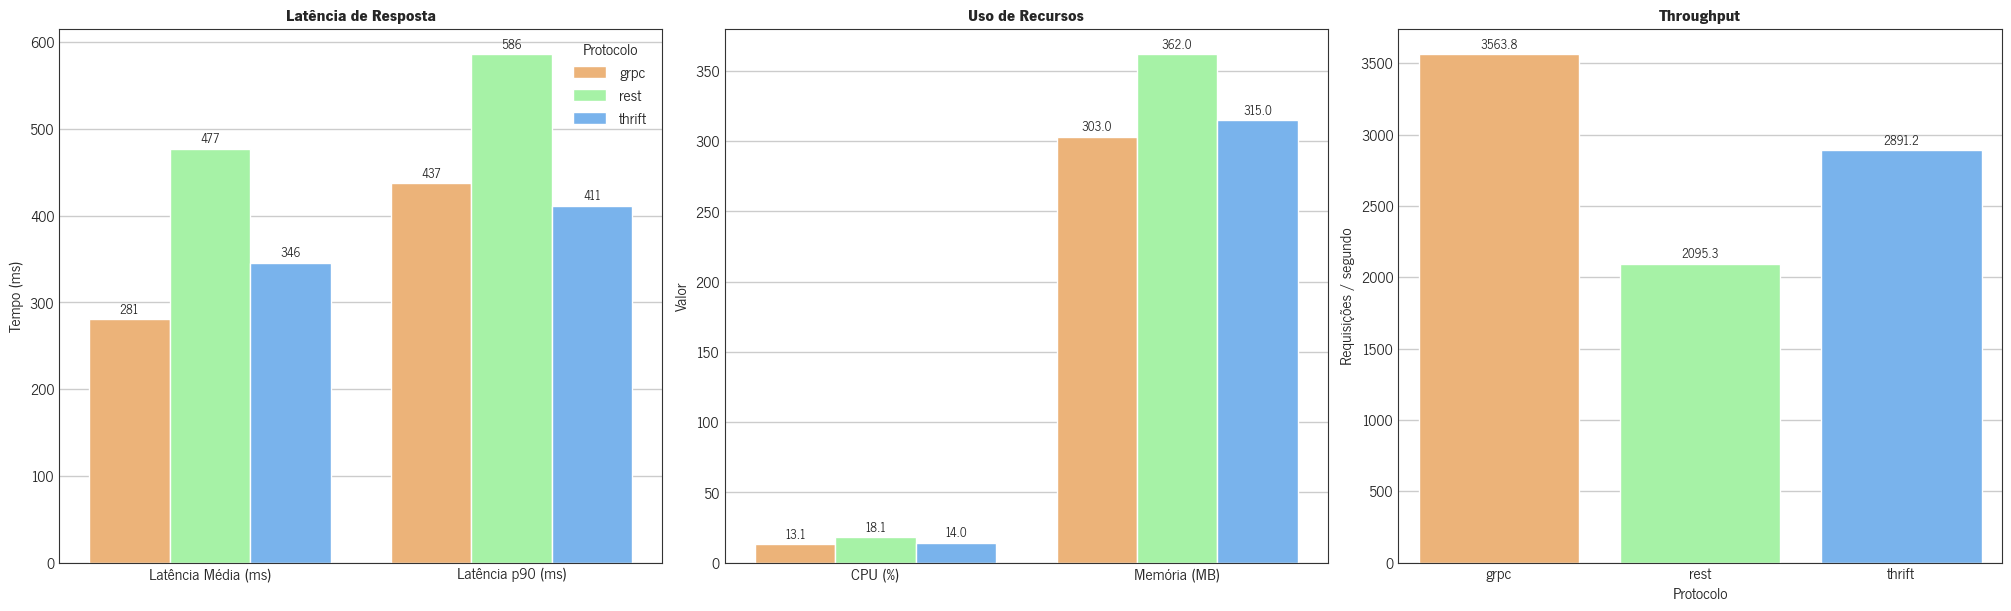
\includegraphics[width=1\linewidth]{imagens/resultados/5-resultados-simples.png}    
    {\par \raggedright \footnotesize Fonte: Elaborado pelo autor.\par}
\end{figure}

\begin{table}[H]
\centering
\caption{Métricas de desempenho e uso de recursos - Cenário Simples}
\label{tab:5-res-simples}
\begin{tabular}[\linewidth]{lrrrrrrr}
\hline
Protocolo & Avg (ms) & Max (ms) & p90 (ms) & p95 (ms) & Throughput (req/s) & CPU (\%) & \acrshort{ram} (MB) \\
\hline
\textbf{\acrshort{grpc}} & 280,60 & 536,43 & 437,34 & 500,18 & 3.563,80 & 13,10 & 303 \\
\textbf{Thrift} & 345,87 & 545,47 & 401,14 & 435,93 & 2.891,20 & 14,00 & 315 \\
\textbf{\gls{rest}} & 477,25 & 653,16 & 510,44 & 512,56 & 2.095,30 & 18,10 & 362 \\
\hline
\end{tabular}
{\par \raggedright \footnotesize Fonte: Elaborado pelo autor.\par}
\end{table}

\subsection{\acrshort{grpc}}

O protocolo \textbf{\acrshort{grpc}} apresentou o melhor desempenho geral no \emph{Cenário Simples}, conforme resumido na \autoref{tab:5-res-simples} e ilustrado na \autoref{fig:5-res-simples}. A \autoref{tab:5-res-simples-grpc} está organizada em colunas que descrevem:

\begin{itemize}
\item \textbf{Avg (ms)}: latência média de resposta;
\item \textbf{Max (ms)}: maior latência observada;
\item \textbf{p90 (ms)} e \textbf{p95 (ms)}: latências de cauda (percentis 90 e 95);
\item \textbf{Throughput (req/s)}: taxa média de requisições por segundo;
\item \textbf{CPU (\%)} e \textbf{\acrshort{ram} (MB)}: consumo médio de recursos.
\end{itemize}

Os valores destacados em \textcolor{green}{verde} correspondem ao melhor desempenho observado (menor latência, maior \emph{throughput} ou menor uso de recursos), enquanto os valores em \textcolor{red}{vermelho} indicam desempenho inferior em relação à métrica. Em número absoluto, apresentam-se os valores do protocolo atual, e nas demais linhas constam as variações $\Delta$~em comparação.

\newcommand{\superior}[1]{\cellcolor{green!12}{#1}}
\newcommand{\inferior}[1]{\cellcolor{red!12}{#1}}

\begin{table}[H]
\centering
\caption{\gls{grpc} comparado com os demais protocolos — Cenário Simples (Thrift/\gls{rest} em $\Delta$\% vs \gls{grpc})}
\label{tab:5-res-simples-grpc}
\begin{tabular}[\linewidth]{lrrrrrrr}
\hline
Protocolo & Avg (ms) & Max (ms) & p90 (ms) & p95 (ms) & Throughput (req/s) & CPU (\%) & \acrshort{ram} (MB) \\
\hline
\textbf{\acrshort{grpc}}   & \superior{\textbf{280,60}} & \superior{\textbf{536,43}} & \inferior{\textbf{437,34}} & \inferior{\textbf{500,18}} & \superior{\textbf{3.563,80}} & \superior{\textbf{13,10}} & \superior{\textbf{303}} \\
\textbf{Thrift} & \inferior{+23,26\%} & \inferior{+1,69\%} & \superior{-8,28\%} & \superior{-12,85\%} & \inferior{-18,87\%} & \inferior{+6,87\%} & \inferior{+3,96\%} \\
\textbf{\gls{rest}}   & \inferior{+70,08\%} & \inferior{+21,76\%} & \inferior{+16,71\%} & \inferior{+2,48\%}  & \inferior{-41,21\%} & \inferior{+38,17\%} & \inferior{+19,47\%} \\
\hline
\end{tabular}
{\par \raggedright \footnotesize Fonte: Elaborado pelo autor.\par}
\end{table}

A análise detalhada das amostras individuais revela que o \gls{grpc} manteve estabilidade notável ao longo das execuções, com baixa dispersão dos valores e ausência de outliers significativos, conforme detalhado na \autoref{tab:5-res-simples-grpc} e visualizado na \autoref{fig:5-simples-grpc-k6}. Essa característica é particularmente valiosa em ambientes de produção, onde a previsibilidade de desempenho é crucial. A eficiência do protocolo \acrshort{http}/2 e a serialização binária através de \textit{Protocol Buffers} evidenciam-se como fatores determinantes para essa performance superior, especialmente em cenários de baixa complexidade onde o overhead de comunicação representa uma parcela significativa do tempo total de processamento.

Em relação ao uso de recursos do servidor, o \gls{grpc} demonstrou eficiência excepcional com apenas 13,10\% de utilização de CPU e 303MB de consumo de memória, como vemos detalhado na \autoref{tab:5-res-simples-grpc}. Esses valores indicam que o protocolo consegue processar as requisições com mínimo impacto nos recursos computacionais, proporcionando uma margem significativa para escalabilidade. A baixa utilização de CPU sugere que a serialização binária e as otimizações do \acrshort{http}/2 reduzem substancialmente o overhead de processamento, enquanto o consumo moderado de memória indica gerenciamento eficiente de buffers e conexões.

\begin{figure}[H]
    \caption{\acrshort{grpc}: Dados de Execução \gls{grpc} (amostragem 15 execuções)}
    \label{fig:5-simples-grpc-k6}
    \centering
    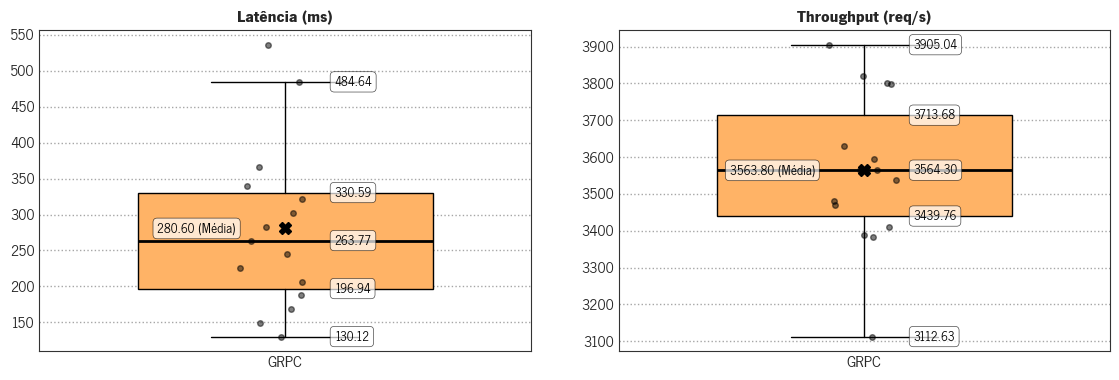
\includegraphics[width=1\linewidth]{imagens//resultados/5-resultados-simples-grpc-k6.png}
    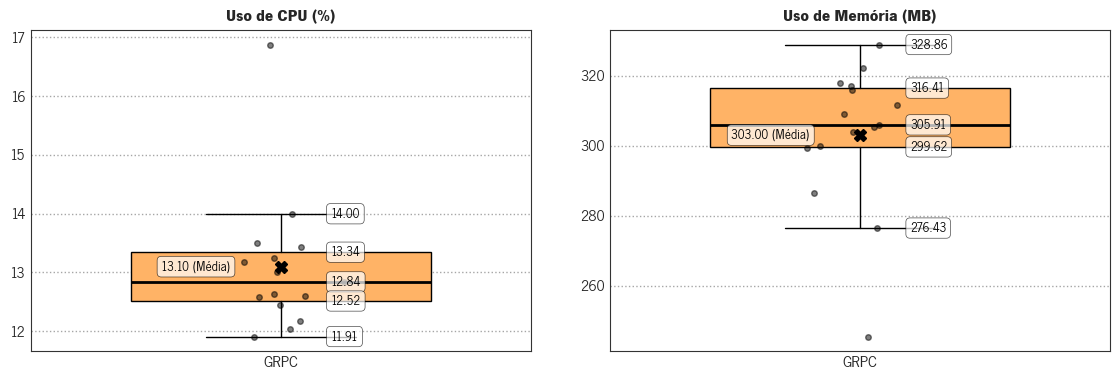
\includegraphics[width=1\linewidth]{imagens//resultados/5-resultados-simples-grpc-prometheus.png}    
    {\par \raggedright \footnotesize Fonte: Elaborado pelo autor.\par}
\end{figure}



\subsection{Thrift}

O Apache Thrift demonstrou desempenho intermediário no cenário simples, com tempo médio de resposta de 345,87 ms, aproximadamente \textbf{23\%} superior ao \gls{grpc}, como se observa na \autoref{tab:5-res-simples}. O tempo máximo registrado foi de 545,47ms, próximo ao observado no \gls{grpc}, sugerindo comportamento similar nos picos de latência. Os percentis de cauda apresentaram valores relevantes, com p90 de 401,14 ms e p95 de 435,93 ms, indicando uma distribuição de latência mais concentrada na faixa inferior em comparação ao tempo máximo. O throughput obtido foi de 2.891,20 req/s, posicionando-se entre o \gls{grpc} e o \gls{rest}.

\begin{table}[H]
\centering
\caption{Thrift comparado com os demais protocolos — Cenário Simples (\acrshort{grpc}/\gls{rest} em $\Delta$\% vs Thrift)}
\label{tab:5-res-simples-thrift}
\begin{tabular}[\linewidth]{lrrrrrrr}
\hline
Protocolo & Avg (ms) & Max (ms) & p90 (ms) & p95 (ms) & Throughput (req/s) & CPU (\%) & \acrshort{ram} (MB) \\
\hline
\textbf{Thrift} & \inferior{\textbf{345,87}} & \inferior{\textbf{545,47}} & \superior{\textbf{401,14}} & \superior{\textbf{435,93}} & \inferior{\textbf{2.891,20}} & \inferior{\textbf{14,00}} & \inferior{\textbf{315}} \\
\textbf{\acrshort{grpc}}   & \superior{-18,87\%} & \superior{-1,66\%} & \inferior{+9,02\%}  & \inferior{+14,74\%} & \superior{+23,26\%} & \superior{-6,43\%} & \superior{-3,81\%} \\
\textbf{\gls{rest}}   & \inferior{+37,99\%} & \inferior{+19,74\%} & \inferior{+27,25\%} & \inferior{+17,58\%} & \inferior{-27,53\%} & \inferior{+29,29\%} & \inferior{+14,92\%} \\
\hline
\end{tabular}
{\par \raggedright \footnotesize Fonte: Elaborado pelo autor.\par}
\end{table}

As amostras individuais do Thrift, conforme observado na \autoref{tab:5-res-simples-thrift} e ilustrado na \autoref{fig:5-simples-Thrift-k6}, revelaram consistência adequada caracterizada por latência média de 345,87 ms com desvio padrão reduzido (28,62 ms), enquanto os percentis de cauda (p90 = 401,14 ms; p95 = 435,93 ms) ficaram próximos ao máximo observado (545,47 ms), indicando baixa dispersão e ausência de outliers extremos. O comportamento observado sugere que a arquitetura do Thrift, com sua serialização binária proprietária que minimiza overhead de parsing e protocolo de transporte TCP direto que garante entrega ordenada com mínimo reenvio, oferece eficiência satisfatória para cenários simples. A diferença de desempenho em relação ao \gls{grpc} pode ser atribuída às otimizações específicas do \acrshort{http}/2, como a multiplexação de streams e cabeçalhos compactados, além da maturidade das implementações de Protocol Buffers, que conferem vantagem técnica ao \gls{grpc} em cenários de comunicação inter-serviços.

O uso de recursos do servidor pelo Thrift mostrou-se ligeiramente superior ao \gls{grpc}, com 14,00\% de utilização de CPU e 315MB de consumo de memória. Embora ainda em patamares baixos, esses valores indicam um overhead discreto em relação ao \gls{grpc}. A diferença na utilização de CPU pode relacionar-se às características específicas da serialização binária do Thrift e ao gerenciamento de conexões TCP, que podem demandar processamento adicional em comparação às otimizações nativas do \acrshort{http}/2.

\begin{figure}[H]
    \caption{Thrift: Dados de Execução (amostragem 15 execuções)}
    \label{fig:5-simples-Thrift-k6}
    \centering
    \includegraphics[width=1\linewidth]{imagens//resultados/5-resultados-simples-Thrift-k6.png}
    \includegraphics[width=1\linewidth]{imagens//resultados/5-resultados-simples-Thrift-prometheus.png}    
    {\par \raggedright \footnotesize Fonte: Elaborado pelo autor.\par}
\end{figure}



\subsection{\gls{rest}}

O protocolo \gls{rest} apresentou o menor desempenho no cenário simples, com tempo médio de resposta de 477,25ms (detalhes na \autoref{tab:5-res-simples-rest}), representando um overhead de aproximadamente \textbf{70\%} em relação ao \gls{grpc}. O tempo máximo observado foi de \textbf{653,16ms}, o mais elevado entre os três protocolos, indicando maior variabilidade de desempenho. Os percentis de cauda confirmam essa tendência, com p90 de \textbf{510,44ms} e p95 de \textbf{512,62ms}, demonstrando distribuição de latência mais concentrada, porém em patamares superiores. O throughput alcançado foi de \textbf{2.095,30 req/s}, o menor entre os protocolos testados.


\begin{table}[H]
\centering
\caption{\gls{rest} comparado com os demais protocolos — Cenário Simples (\acrshort{grpc}/Thrift em \Delta\% vs \gls{rest})}
\label{tab:5-res-simples-rest}
\begin{tabular}[\linewidth]{lrrrrrrr}
\hline
Protocolo & Avg (ms) & Max (ms) & p90 (ms) & p95 (ms) & Throughput (req/s) & CPU (\%) & \acrshort{ram} (MB) \\
\hline
\textbf{\gls{rest}}   & \inferior{\textbf{477,25}} & \inferior{\textbf{653,16}} & \inferior{\textbf{510,44}} & \inferior{\textbf{512,56}} & \inferior{\textbf{2.095,30}} & \inferior{\textbf{18,10}} & \inferior{\textbf{362}} \\
\textbf{\acrshort{grpc}}   & \superior{-41,20\%} & \superior{-17,87\%} & \superior{-14,32\%} & \superior{-2,42\%}  & \superior{+70,09\%} & \superior{-27,62\%} & \superior{-16,30\%} \\
\textbf{Thrift} & \superior{-27,53\%} & \superior{-16,49\%} & \superior{-21,41\%} & \superior{-14,95\%} & \superior{+37,99\%} & \superior{-22,65\%} & \superior{-12,98\%} \\
\hline
\end{tabular}
{\par \raggedright \footnotesize Fonte: Elaborado pelo autor.\par}
\end{table}

O consumo de recursos do servidor pelo \gls{rest}, conforme observamos na \autoref{fig:5-res-simples-rest} foi o mais elevado no cenário simples, com \textbf{18,10\%} de utilização de CPU e \textbf{362MB} de consumo de memória. Esses valores refletem o overhead inerente ao processamento de \acrshort{json} e às características do protocolo \acrshort{http}/1.1. A maior utilização de CPU indica que a serialização e desserialização de texto exigem mais ciclos de processamento em comparação aos formatos binários, enquanto o maior consumo de memória pode estar relacionado ao armazenamento temporário de strings \acrshort{json} e buffers de rede menos otimizados.

A análise das execuções individuais do \gls{rest}, conforme detalhado na \autoref{tab:5-res-simples-rest} e ilustrado na \autoref{fig:5-res-simples-rest}, revela comportamento previsível, com desempenho consistentemente inferior aos protocolos binários. Apesar da performance inferior, o \gls{rest} mantém uma estabilidade adequada, com tempos mantendo uma variação mínima e quantidade de throughput acima dos dois mil por segundo, confirmando sua viabilidade para cenários em que se prioriza a simplicidade de implementação e a interoperabilidade em detrimento da eficiência de comunicação. O comportamento observado alinha-se com as expectativas teóricas sobre protocolos baseados em texto versus protocolos binários em cenários de comunicação inter-serviços.

\begin{figure}[H]
    \caption{Rest: Dados de Execução (amostragem 15 execuções)}
    \label{fig:5-res-simples-rest}
    \centering
    \includegraphics[width=1\linewidth]{imagens//resultados/5-resultados-simples-Rest-k6.png}
    \includegraphics[width=1\linewidth]{imagens//resultados/5-resultados-simples-Rest-prometheus.png}    
    {\par \raggedright \footnotesize Fonte: Elaborado pelo autor.\par}
\end{figure}



\section{Cenário Tradicional}

Como descrito no \autoref{ch:4metodologia}, o cenário tradicional representa consultas de complexidade intermediária, exigindo processamento mais intensivo pelo módulo de \acrfull{ia} e maior troca de dados entre os microsserviços. As 15 execuções realizadas para cada protocolo revelam comportamentos distintos em condições de demanda moderada, em que tanto o processamento computacional quanto a comunicação inter-serviços contribuem significativamente para o tempo total de resposta. Analisando os dados detalhados na \autoref{tab:5-res-tradicioanl} e ilustrados comparativamente na \autoref{fig:5-res-tradicioanl}, observa-se, do lado do cliente, um aumento considerável nos tempos de resposta e a correspondente redução no \textit{throughput}. Do lado do servidor, o consumo de recursos cresce substancialmente, refletindo a maior demanda computacional do processamento de \gls{ia}.

\begin{figure}[H]
    \caption{Resultados Comparativos - Cenário Tradicional}
    \label{fig:5-res-tradicioanl}
    \centering
    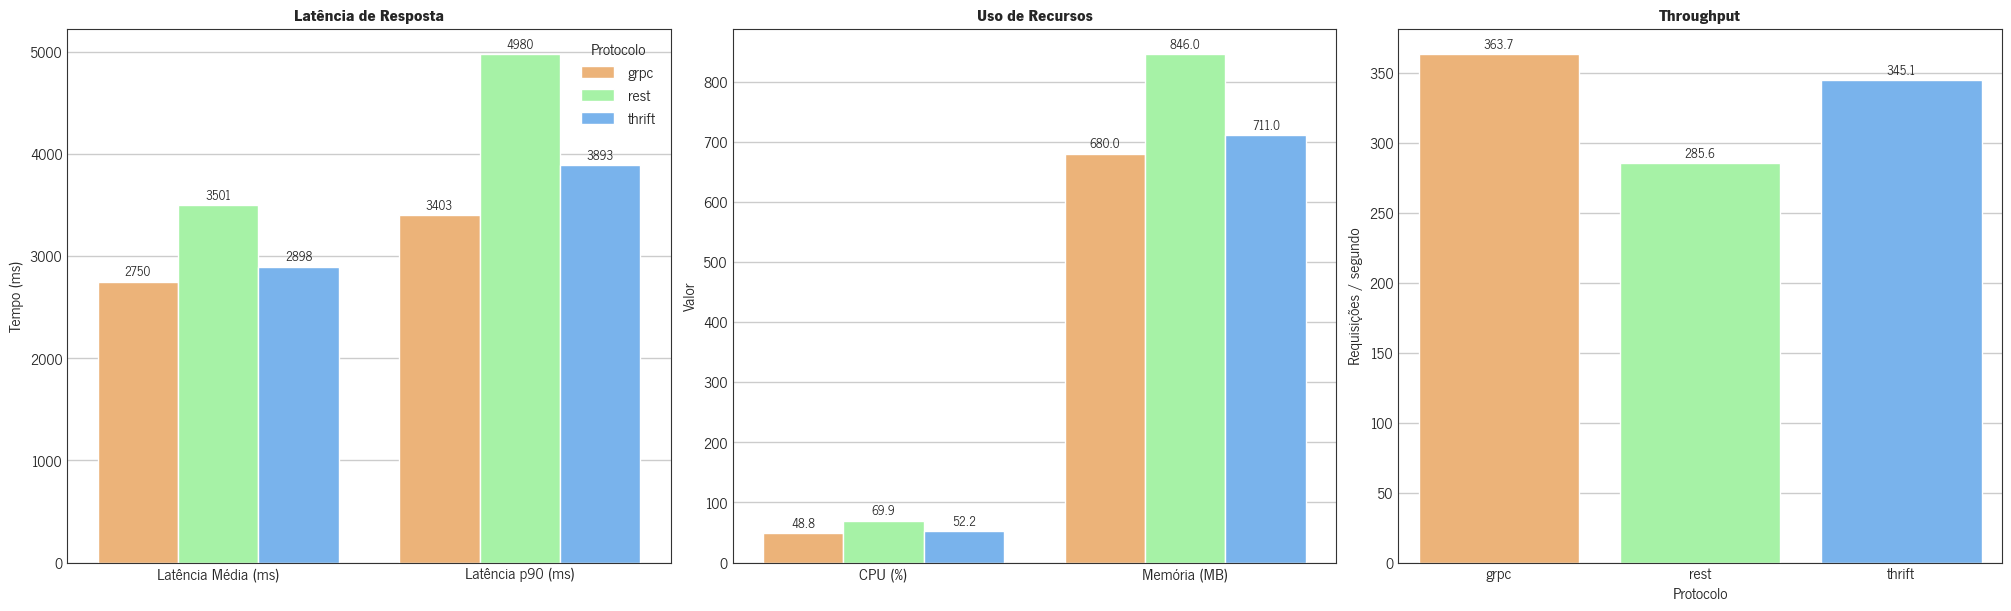
\includegraphics[width=1\linewidth]{imagens/resultados/5-resultados-tradicional.png}    
    {\par \raggedright \footnotesize Fonte: Elaborado pelo autor.\par}
\end{figure}


\begin{table}[H]
\centering
\caption{Métricas de desempenho e uso de recursos - Cenário Tradicional}
\label{tab:5-res-tradicioanl}
\begin{tabular}[\linewidth]{lrrrrrrr}
\hline
Protocolo & Avg (ms) & Max (ms) & p90 (ms) & p95 (ms) & Throughput (req/s) & CPU (\%) & \acrshort{ram} (MB) \\
\hline
\textbf{\acrshort{grpc}}   & 2.749,80 & 3.440,36 & 3.396,90 & 3.401,73 & 363,70 & 48,80 & 680 \\
\textbf{Thrift} & 2.897,87 & 3.969,82 & 3.892,62 & 3.923,65 & 345,10 & 52,20 & 711 \\
\textbf{\gls{rest}}   & 3.501,06 & 5.372,78 & 4.980,34 & 5.175,86 & 285,60 & 69,90 & 846 \\
\hline
\end{tabular}
{\par \raggedright \footnotesize Fonte: Elaborado pelo autor.\par}
\end{table}

\subsection{\acrshort{grpc}}

No cenário tradicional, o \gls{grpc} manteve sua posição de liderança em desempenho, registrando tempo médio de resposta de 2.749,80ms. O tempo máximo observado foi de 3.440,36ms, demonstrando que mesmo sob carga moderada, o protocolo mantém variabilidade controlada. Os percentis de cauda evidenciam comportamento robusto, com p90 de 3.396,90ms e p95 de 3.401,73ms, indicando distribuição de latência concentrada próxima ao valor máximo. O throughput foi de 363,70 req/s, uma redução significativa em relação ao cenário simples, mas ainda superior aos demais protocolos.

\begin{table}[H]
\centering
\caption{\gls{grpc} comparado com os demais protocolos — Cenário Tradicional (Thrift/\gls{rest} em $\Delta$\% vs \gls{grpc})}
\label{tab:5-res-tradicional-grpc}
\makebox[\textwidth][c]{%
\begin{tabular}{lrrrrrrr}
\hline
Protocolo & Avg (ms) & Max (ms) & p90 (ms) & p95 (ms) & Throughput (req/s) & CPU (\%) & \acrshort{ram} (MB) \\
\hline
\textbf{\acrshort{grpc}}   & \superior{\textbf{2.749,80}} & \superior{\textbf{3.440,36}} & \superior{\textbf{3.396,90}} & \superior{\textbf{3.401,73}} & \superior{\textbf{363,70}} & \superior{\textbf{48,80}} & \superior{\textbf{680}} \\
\textbf{Thrift} & \inferior{+5,40\%}  & \inferior{+15,38\%} & \inferior{+14,58\%} & \inferior{+15,35\%} & \inferior{-5,10\%}  & \inferior{+6,97\%}  & \inferior{+4,56\%} \\
\textbf{\gls{rest}}   & \inferior{+27,29\%} & \inferior{+56,15\%} & \inferior{+46,64\%} & \inferior{+52,19\%} & \inferior{-21,45\%} & \inferior{+43,23\%} & \inferior{+24,41\%} \\
\hline
\end{tabular}%
}
{\par \raggedright \footnotesize Fonte: Elaborado pelo autor.\par}
\end{table}


As execuções individuais, conforme apresentado na \autoref{tab:5-res-tradicional-grpc} e visualizado na \autoref{fig:5-Tradicional-gRPC-k6}, revelam que o \gls{grpc} escalou de forma linear e previsível em relação ao cenário simples, mantendo a eficiência de comunicação mesmo com payloads maiores e processamento mais intensivo. A diferença entre o tempo médio e os percentis de cauda sugere que o protocolo consegue absorver adequadamente os picos de processamento sem degradação significativa da performance. Essa característica é fundamental em aplicações financeiras, onde a consistência de resposta é tão importante quanto a velocidade absoluta, especialmente durante períodos de maior demanda computacional.

\begin{figure}[H]
    \caption{\acrshort{grpc}: Dados de Execução no Cenário Tradicional (amostragem 15 execuções)}
    \label{fig:5-Tradicional-gRPC-k6}
    \centering
    \includegraphics[width=1\linewidth]{imagens//resultados/5-resultados-Tradicional-gRPC-k6.png}
    \includegraphics[width=1\linewidth]{imagens//resultados/5-resultados-Tradicional-gRPC-prometheus.png}    
    {\par \raggedright \footnotesize Fonte: Elaborado pelo autor.\par}
\end{figure}


O uso de recursos do servidor aumentou substancialmente em relação ao cenário anterior, com 48,80\% de utilização de CPU e 680 MB de consumo de memória. Esses valores refletem a maior demanda computacional do processamento de \gls{ia}, mas ainda demonstram eficiência relativa do \gls{grpc}. A utilização de CPU próxima de 50\% indica que o sistema está operando em uma faixa adequada, com margem para picos de demanda, enquanto o consumo de memória duplicou em relação ao cenário simples, comportamento esperado devido ao maior volume de dados processados, os dados das execuções. Detalhes de todas as execuções podem ser vistas na  \autoref{fig:5-Tradicional-gRPC-k6}.

\subsection{Thrift}

O Apache Thrift apresentou tempo médio de resposta de 2.897,87ms no cenário tradicional, mantendo uma diferença de aproximadamente 5\% em relação ao \gls{grpc}. O tempo máximo registrado foi de 3.969,82ms, superior ao \gls{grpc}, indicando maior sensibilidade a picos de processamento. Os percentis de cauda mostram p90 de 3.892,62ms e p95 de 3.923,65ms, evidenciando distribuição de latência mais dispersa. O throughput foi de 345,10 req/s, ligeiramente inferior ao \gls{grpc}.

\begin{table}[H]
\centering
\caption{Thrift comparado com os demais protocolos — Cenário Tradicional (\acrshort{grpc}/\gls{rest} em $\Delta$\% vs Thrift)}
\label{tab:5-res-tradicional-thrift}
\makebox[\textwidth][c]{%
\begin{tabular}{lrrrrrrr}
\hline
Protocolo & Avg (ms) & Max (ms) & p90 (ms) & p95 (ms) & Throughput (req/s) & CPU (\%) & \acrshort{ram} (MB) \\
\hline
\textbf{Thrift} & \textbf{2.897,87} & \textbf{3.969,82} & \textbf{3.892,62} & \textbf{3.923,65} & \textbf{345,10} & \textbf{52,20} & \textbf{711} \\
\textbf{\acrshort{grpc}}   & \superior{-5,10\%}  & \superior{-13,36\%} & \superior{-12,73\%} & \superior{-13,30\%} & \superior{+5,39\%} & \superior{-6,51\%} & \superior{-4,36\%} \\
\textbf{\gls{rest}}   & \inferior{+20,83\%} & \inferior{+35,34\%} & \inferior{+27,93\%} & \inferior{+31,86\%} & \inferior{-17,23\%} & \inferior{+33,91\%} & \inferior{+19,01\%} \\
\hline
\end{tabular}%
}
{\par \raggedright \footnotesize Fonte: Elaborado pelo autor.\par}
\end{table}

A análise das amostras individuais do Thrift, conforme detalhado na \autoref{tab:5-res-tradicional-thrift} e visualizado na \autoref{fig:5-Tradicional-Thrift-k6}, revela comportamento estável, porém apresenta maior variabilidade em comparação ao \gls{grpc}. O protocolo demonstra escalabilidade adequada, mas evidencia sensibilidade superior às variações na carga de processamento. A diferença pronunciada nos valores máximos e percentis superiores sugere que o Thrift pode ser mais suscetível a gargalos em cenários de processamento intensivo, possivelmente relacionados a suas estratégias de buffering e ao gerenciamento das conexões \acrshort{tcp}.

\begin{figure}[H]
    \caption{Thrift: Dados de Execução no Cenário Tradicional (amostragem 15 execuções)}
    \label{fig:5-Tradicional-Thrift-k6}
    \centering
    \includegraphics[width=1\linewidth]{imagens//resultados/5-resultados-Tradicional-Thrift-k6.png}
    \includegraphics[width=1\linewidth]{imagens//resultados/5-resultados-Tradicional-Thrift-prometheus.png}    
    {\par \raggedright \footnotesize Fonte: Elaborado pelo autor.\par}
\end{figure}

O consumo de recursos do servidor apresentou 52,20\% de utilização de CPU e 711 MB de consumo de memória. Comparado ao \gls{grpc}, o Thrift apresentou overhead adicional de aproximadamente 7\% na CPU e 4\% na memória, esse número continua a tendência observada no cenário simples. Essa diferença pode estar relacionada às características específicas do protocolo \acrshort{tcp} direto e às estratégias de serialização do Thrift, que podem exigir processamento adicional em cenários de maior complexidade computacional.

\subsection{\gls{rest}}

O protocolo \gls{rest} registrou um tempo médio de resposta de 3.501,06 ms no cenário tradicional, enquanto Thrift e \acrshort{grpc} apresentaram diferenças de -17,23\% e -21,46\%, respectivamente. O tempo máximo observado foi significativamente elevado, atingindo 5.372,78 ms, indicando maior variabilidade de desempenho. Os percentis de cauda confirmam essa tendência, com p90 de 4.980,34ms e p95 de 5.175,86ms. O throughput alcançou 285,60 req/s; embora tenha sido o menor valor, permaneceu muito próximo dos demais.

\begin{table}[H]
\centering
\caption{\gls{rest} comparado com os demais protocolos — Cenário Tradicional ($\Delta$\% vs \gls{rest})}
\label{tab:5-res-tradicional-rest}
\makebox[\textwidth][c]{%
\begin{tabular}{lrrrrrrr}
\hline
Protocolo & Avg (ms) & Max (ms) & p90 (ms) & p95 (ms) & Throughput (req/s) & CPU (\%) & \acrshort{ram} (MB) \\
\hline
\textbf{\gls{rest}}   & \inferior{\textbf{3.501,06}} & \inferior{\textbf{5.372,78}} & \inferior{\textbf{4.980,34}} & \inferior{\textbf{5.175,86}} & \inferior{\textbf{285,60}} & \inferior{\textbf{69,90}} & \inferior{\textbf{846}} \\
\textbf{\acrshort{grpc}}   & \superior{-21,46\%} & \superior{-35,97\%} & \superior{-31,79\%} & \superior{-34,26\%} & \superior{+27,35\%} & \superior{-30,19\%} & \superior{-19,62\%} \\
\textbf{Thrift} & \superior{-17,23\%} & \superior{-26,11\%} & \superior{-21,78\%} & \superior{-24,19\%} & \superior{+20,83\%} & \superior{-25,32\%} & \superior{-15,96\%} \\
\hline
\end{tabular}%
}
{\par \raggedright \footnotesize Fonte: Elaborado pelo autor.\par}
\end{table}

As execuções individuais do \gls{rest} evidenciam o impacto cumulativo do overhead de serialização \acrshort{json} e protocolo \acrshort{http}/1.1 em cenários de maior complexidade. A diferença mais acentuada entre o tempo médio e os valores de cauda, conforme apresentado na \autoref{tab:5-res-tradicional-rest} e visualizada detalhadamente na \autoref{fig:5-Tradicional-REST-k6}, sugere que o \gls{rest} é especialmente sensível a variações na carga de processamento e no tamanho dos payloads. Essa característica pode representar um desafio em aplicações financeiras que requerem previsibilidade de desempenho, especialmente durante períodos de alta demanda em que a latência de cauda pode impactar significativamente a experiência do usuário.

\begin{figure}[H]
    \caption{\gls{rest}: Dados de Execução no Cenário Tradicional (amostragem 15 execuções)}
    \label{fig:5-Tradicional-REST-k6}
    \centering
    \includegraphics[width=1\linewidth]{imagens//resultados/5-resultados-Tradicional-REST-k6.png}
    \includegraphics[width=1\linewidth]{imagens//resultados/5-resultados-Tradicional-REST-prometheus.png}    
    {\par \raggedright \footnotesize Fonte: Elaborado pelo autor.\par}
\end{figure}

O uso de recursos do servidor pelo \gls{rest} foi significativamente superior, com 69,90\% de utilização de CPU e 846MB de consumo de memória. O Thrift por exemplo, utilizou 25,32\% a menos de CPU total. A elevada utilização de CPU indica que o processamento de \acrshort{json} e as características do \acrshort{http}/1.1 se tornam gargalos significativos em cenários de maior complexidade, enquanto o maior consumo de memória reflete o overhead das estruturas de dados textuais.

\section{Cenário Complexo}

O cenário complexo é o teste de estresse mais rigoroso, envolvendo consultas que exigem processamento intensivo de dados históricos e síntese avançada de informações pelo módulo de \acrfull{ia}. As 15 execuções neste cenário destacam o desempenho dos protocolos sob condições próximas aos limites operacionais, testando tanto o processamento computacional quanto a eficiência de comunicação ao extremo. No lado do cliente, há uma convergência dos tempos de resposta em relação aos \textit{timeouts} configurados, enquanto no lado do servidor, o uso de recursos se aproxima da saturação, especialmente para os protocolos menos eficientes. No entanto, as discrepâncias na eficiência de recursos e no \textit{throughput} persistiram, conforme ilustrado na \autoref{fig:resultados_complexo} e na \autoref{tab:res_complexo}.



\begin{figure}[H]
    \caption{Resultados Comparativos - Cenário Complexo}
    \label{fig:resultados_complexo}
    \centering
    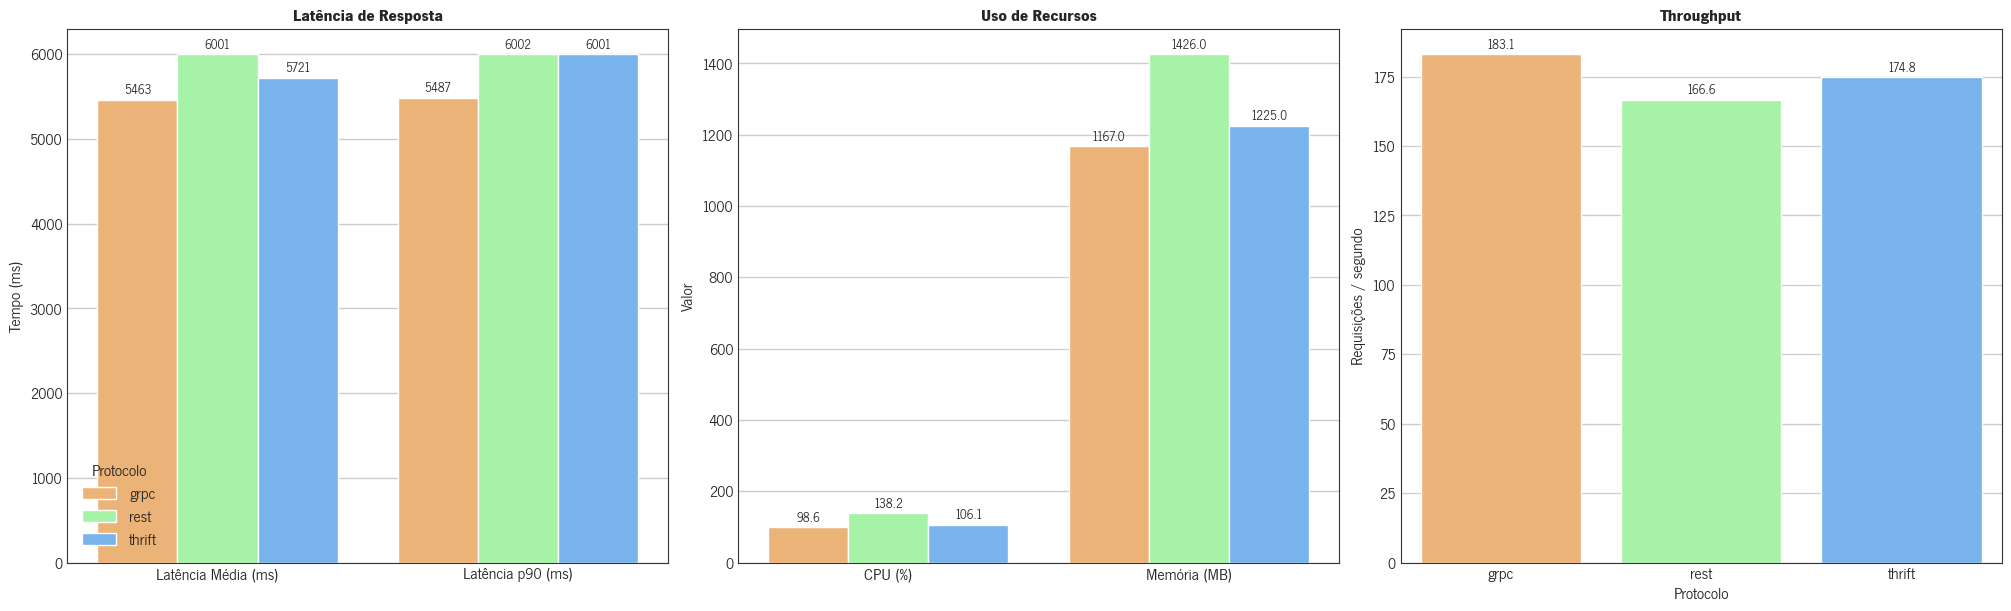
\includegraphics[width=1\linewidth]{imagens/resultados/5-resultados-complexo.png}    
    {\par \raggedright \footnotesize Fonte: Elaborado pelo autor.\par}
\end{figure}


\begin{table}[H]
\centering
\caption{Métricas de desempenho e uso de recursos - Cenário Complexo}
\label{tab:res_complexo}
\begin{tabular}[\linewidth]{lrrrrrrr}
\hline
Protocolo & Avg (ms) & Max (ms) & p90 (ms) & p95 (ms) & Throughput (req/s) & CPU (\%) & \acrshort{ram} (MB) \\
\hline
\textbf{\acrshort{grpc}}   & 5.462,68 & 5.499,37 & 5.486,74 & 5.490,84 & 183,10 & 98,60 & 1.167 \\
\textbf{Thrift} & 5.721,15 & 6.000,96 & 6.000,58 & 6.000,76 & 174,80 & 106,10 & 1.225 \\
\textbf{\gls{rest}}   & 6.000,97 & 6.002,16 & 6.001,80 & 6.001,84 & 166,60 & 138,20 & 1.426 \\
\hline
\end{tabular}
{\par \raggedright \footnotesize Fonte: Elaborado pelo autor.\par}
\end{table}

\subsection{\acrshort{grpc}}

No cenário complexo, o \gls{grpc} apresentou tempo médio de resposta de 5.462,68ms, mantendo sua eficiência relativa mesmo sob alta carga computacional. O tempo máximo observado foi de 5.499,37ms, demonstrando baixa variabilidade e comportamento altamente previsível. Os percentis de cauda evidenciam consistência excepcional, com p90 de 5.486,74ms e p95 de 5.490,84ms, valores muito próximos à média e ao máximo. O throughput foi de 183,10 req/s, ainda o melhor desempenho entre os protocolos testados (ver \autoref{tab:5-res-complexo-grpc}).

\begin{table}[H]
\centering
\caption{\gls{grpc} comparado com os demais protocolos — Cenário Complexo (Thrift/\gls{rest} em $\Delta$\% vs \gls{grpc})}
\label{tab:5-res-complexo-grpc}
\makebox[\textwidth][c]{%
\begin{tabular}{lrrrrrrr}
\hline
Protocolo & Avg (ms) & Max (ms) & p90 (ms) & p95 (ms) & Throughput (req/s) & CPU (\%) & \acrshort{ram} (MB) \\
\hline
\textbf{\acrshort{grpc}}   & \superior{\textbf{5.462,68}} & \superior{\textbf{5.499,37}} & \superior{\textbf{5.486,74}} & \superior{\textbf{5.490,84}} & \superior{\textbf{183,10}} & \superior{\textbf{98,60}} & \superior{\textbf{1.167}} \\
\textbf{Thrift} & \inferior{+4,73\%}  & \inferior{+9,14\%}  & \inferior{+9,35\%}  & \inferior{+9,30\%}  & \inferior{-4,53\%}  & \inferior{+7,61\%}  & \inferior{+4,97\%} \\
\textbf{\gls{rest}}   & \inferior{+9,87\%}  & \inferior{+9,14\%}  & \inferior{+9,38\%}  & \inferior{+9,32\%}  & \inferior{-9,02\%}  & \inferior{+40,21\%} & \inferior{+22,23\%} \\
\hline
\end{tabular}%
}
{\par \raggedright \footnotesize Fonte: Elaborado pelo autor.\par}
\end{table}

A análise das execuções individuais, conforme apresentado na \autoref{tab:5-res-complexo-grpc} e visualizado na \autoref{fig:5-Complexo-gRPC-k6}, revela que o \gls{grpc} manteve estabilidade notável mesmo no cenário mais exigente, com todas as amostras concentradas em uma faixa estreita de valores. Essa característica sugere que o protocolo consegue otimizar eficientemente a comunicação inter-serviços mesmo quando o processamento de \gls{ia} representa a maior parte do tempo de resposta. A baixa dispersão dos valores indica que o \gls{grpc} oferece previsibilidade superior em cenários críticos, aspecto fundamental para sistemas financeiros que operam com \acrshort{sla}s rigorosos e requerem comportamento determinístico.

\begin{figure}[H]
    \caption{\acrshort{grpc}: Dados de Execução no Cenário Complexo (amostragem 15 execuções)}
    \label{fig:5-Complexo-gRPC-k6}
    \centering
    \includegraphics[width=1\linewidth]{imagens//resultados/5-resultados-Complexo-gRPC-k6.png}
    \includegraphics[width=1\linewidth]{imagens//resultados/5-resultados-Complexo-gRPC-prometheus.png}    
    {\par \raggedright \footnotesize Fonte: Elaborado pelo autor.\par}
\end{figure}

O uso de recursos do servidor atingiu 98,60\% de utilização de CPU e 1.167MB de consumo de memória, indicando operação próxima aos limites, mas ainda de forma controlada. Mesmo sob alta carga, o \gls{grpc} conseguiu manter eficiência relativa, evitando saturação completa dos recursos. O consumo de memória, embora elevado, permaneceu em patamares gerenciáveis, variando entre 1.076 MB e 1.248 MB, demonstrando que o protocolo lida com grandes volumes de dados de forma otimizada.

\subsection{Thrift}

O Apache Thrift registrou tempo médio de resposta de 5.721,15ms no cenário complexo, representando um overhead de aproximadamente 5\% em relação ao \gls{grpc}. O tempo máximo observado foi de 6.000,96ms, coincidindo com os percentis de cauda que apresentaram p90 de 6.000,58ms e p95 de 6.000,76ms, todos próximos ao limite de \textit{timeout} configurado (conforme estruturado em \autoref{sec:5-metricas-variaveis}). O throughput foi de 174,80 req/s, inferior ao \gls{grpc} mas ainda competitivo.

\begin{table}[H]
\centering
\caption{Thrift comparado com os demais protocolos — Cenário Complexo (\acrshort{grpc}/\gls{rest} em $\Delta$\% vs Thrift)}
\label{tab:5-res-complexo-thrift}
\makebox[\textwidth][c]{%
\begin{tabular}{lrrrrrrr}
\hline
Protocolo & Avg (ms) & Max (ms) & p90 (ms) & p95 (ms) & Throughput (req/s) & CPU (\%) & \acrshort{ram} (MB) \\
\hline
\textbf{Thrift} & \textbf{5.721,15} & \textbf{6.000,96} & \textbf{6.000,58} & \textbf{6.000,76} & \textbf{174,80} & \textbf{106,10} & \textbf{1.225} \\
\textbf{\acrshort{grpc}}   & \superior{-4,52\%}  & \superior{-8,37\%}  & \superior{-8,54\%}  & \superior{-8,46\%}  & \superior{+4,75\%}  & \superior{-7,06\%}  & \superior{-4,74\%} \\
\textbf{\gls{rest}}   & \inferior{+4,90\%}  & \inferior{+0,20\%}  & \inferior{+0,02\%}  & \inferior{+0,02\%}  & \inferior{-4,69\%}  & \inferior{+30,27\%} & \inferior{+16,41\%} \\
\hline
\end{tabular}%
}
{\par \raggedright \footnotesize Fonte: Elaborado pelo autor.\par}
\end{table}

As amostras individuais do Thrift, conforme detalhado na \autoref{tab:5-res-complexo-thrift} e visualizado na \autoref{fig:5-Complexo-Thrift-k6}, revelam um padrão interessante, em que várias execuções atingiram valores próximos ao \textit{timeout} configurado, sugerindo que o protocolo aproximou-se de seus limites operacionais neste cenário. Essa característica indica que o Thrift, embora eficiente em cenários simples e tradicionais, pode enfrentar desafios em situações de extrema complexidade computacional. O comportamento observado sugere possível saturação das conexões \acrshort{tcp} ou limitações no gerenciamento de buffers durante processamento intensivo, aspectos que devem ser considerados em implementações de produção.

\begin{figure}[H]
    \caption{Thrift: Dados de Execução no Cenário Complexo (amostragem 15 execuções)}
    \label{fig:5-Complexo-Thrift-k6}
    \centering
    \includegraphics[width=1\linewidth]{imagens//resultados/5-resultados-Complexo-Thrift-k6.png}
    \includegraphics[width=1\linewidth]{imagens//resultados/5-resultados-Complexo-Thrift-prometheus.png}    
    {\par \raggedright \footnotesize Fonte: Elaborado pelo autor.\par}
\end{figure}


O consumo de recursos atingiu 106,10\% de utilização de CPU e 1.225MB de consumo de memória, indicando saturação dos recursos computacionais. A utilização de CPU superior a 100\% sugere que o sistema operou em condições de stress, possivelmente utilizando recursos de múltiplos cores de forma intensiva. O maior consumo de memória em relação ao \gls{grpc} pode estar relacionado a estratégias menos otimizadas de gerenciamento de buffers durante processamento intensivo.

\subsection{\gls{rest}}

O protocolo \gls{rest} apresentou tempo médio de resposta de 6.000,97 ms no cenário complexo, atingindo consistentemente valores próximos ao limite de \textit{timeout}. O tempo máximo registrado foi de 6.002,16 ms, com percentis p90 e p95 de 6.001,80 ms e 6.001,84 ms respectivamente, todos concentrados no limite superior configurado. O throughput foi de 166,60 req/s, o menor entre os três protocolos.

\begin{table}[H]
\centering
\caption{\gls{rest} comparado com os demais protocolos — Cenário Complexo (\acrshort{grpc}/Thrift em $\Delta$\% vs \gls{rest})}
\label{tab:5-res-complexo-rest}
\makebox[\textwidth][c]{%
\begin{tabular}{lrrrrrrr}
\hline
Protocolo & Avg (ms) & Max (ms) & p90 (ms) & p95 (ms) & Throughput (req/s) & CPU (\%) & \acrshort{ram} (MB) \\
\hline
\textbf{\gls{rest}}   & \inferior{\textbf{6.000,97}} & \inferior{\textbf{6.002,16}} & \inferior{\textbf{6.001,80}} & \inferior{\textbf{6.001,84}} & \inferior{\textbf{166,60}} & \inferior{\textbf{138,20}} & \inferior{\textbf{1.426}} \\
\textbf{\acrshort{grpc}}   & \superior{-8,96\%}  & \superior{-8,37\%}  & \superior{-8,55\%}  & \superior{-8,51\%}  & \superior{+9,90\%}  & \superior{-28,67\%} & \superior{-18,19\%} \\
\textbf{Thrift} & \superior{-4,66\%}  & \superior{-0,02\%}  & \superior{-0,02\%}  & \superior{-0,02\%}  & \superior{+4,92\%}  & \superior{-23,25\%} & \superior{-14,11\%} \\
\hline
\end{tabular}%
}
{\par \raggedright \footnotesize Fonte: Elaborado pelo autor.\par}
\end{table}

A análise das execuções do \gls{rest}, conforme apresentado na \autoref{tab:5-res-complexo-rest} e visualizado na \autoref{fig:5-Complexo-REST-k6}, no cenário complexo revela que o protocolo atingiu sistematicamente seus limites operacionais, com praticamente todas as amostras próximas ao \textit{timeout} configurado. Esse comportamento indica que o overhead cumulativo da serialização \acrshort{json} e do protocolo \acrshort{http}/1.1 se torna crítico em cenários de alta complexidade computacional. Os resultados sugerem que o \gls{rest} pode não ser adequado para aplicações que requerem processamento intensivo de \gls{ia} em tempo real, especialmente quando múltiplos microsserviços precisam trocar grandes volumes de dados de forma eficiente.

\begin{figure}[H]
    \caption{\gls{rest}: Dados de Execução no Cenário Complexo (amostragem 15 execuções)}
    \label{fig:5-Complexo-REST-k6}
    \centering
    \includegraphics[width=1\linewidth]{imagens//resultados/5-resultados-Complexo-REST-k6.png}
    \includegraphics[width=1\linewidth]{imagens//resultados/5-resultados-Complexo-REST-prometheus.png}    
    {\par \raggedright \footnotesize Fonte: Elaborado pelo autor.\par}
\end{figure}


O uso de recursos do servidor foi o mais elevado, com 138,20\% de utilização de CPU e 1.426MB de consumo de memória, indicando saturação completa do sistema. A utilização de CPU muito superior a 100\% demonstra que o protocolo \gls{rest} exigiu recursos computacionais além da capacidade disponível, resultando em degradação significativa de performance. O maior consumo de memória entre todos os protocolos reflete o overhead das estruturas de dados textuais e o gerenciamento menos eficiente de buffers em condições extremas.

\section{Análise Geral}

A análise comparativa dos três cenários, conforme observada detalhadamente na \autoref{tab:res_todos_agrupados}, revela padrões consistentes de desempenho que se alinham com as características técnicas fundamentais de cada protocolo. O \gls{grpc} demonstrou superioridade em todos os cenários, mantendo os menores tempos médios de resposta, maior throughput e menor variabilidade, evidenciada por valores próximos entre média, percentis de cauda e máximos. Essa característica de previsibilidade é particularmente valiosa em sistemas financeiros, onde \acrshort{sla}s rigorosos demandam comportamento determinístico. Em termos de recursos, o \gls{grpc} manteve o menor consumo de CPU e memória em todos os cenários, evidenciando eficiência operacional superior. O Thrift apresentou desempenho intermediário satisfatório nos cenários simples e tradicional, mas evidenciou limitações significativas no cenário complexo, onde a utilização de CPU ultrapassou 100\%, indicando saturação dos recursos. O \gls{rest}, embora funcional em todos os cenários, demonstrou degradação progressiva de desempenho, culminando em saturação sistemática no cenário complexo com 138\% de utilização de CPU.

\begin{table}[H]
\centering
\caption{Métricas (média e p95) por cenário e protocolo}
\label{tab:res_todos_agrupados},
\setlength{\tabcolsep}{4pt}
\renewcommand{\arraystretch}{1.15}
\begin{tabularx}{\linewidth}{l X | r | r | r | r | r | r | r | r |}
\hline
\multicolumn{2}{c}{} & \multicolumn{2}{c}{\textbf{Latência (ms)}} & \multicolumn{2}{c}{\textbf{Vazão (req/s)}} & \multicolumn{2}{c}{\textbf{CPU (\%)}} & \multicolumn{2}{c}{\textbf{\acrshort{ram} (MB)}} \\
\cline{3-10}
\textbf{Cenário} & \textbf{Prot.} & Avg & p95 & Avg & p95 & Avg & p95 & Avg & p95 \\
\hline
\multirow{3}{*}{Simples}
  & \textbf{\acrshort{grpc}}   & 280,60   & 500,18   & 3.563,80 & 3.845,10 & 13,10  & 14,86  & 303   & 324  \\
  & \textbf{Thrift} & 345,87   & 457,20   & 2.891,20 & 3.156,78 & 14,00  & 15,48  & 315   & 343  \\
  & \textbf{\gls{rest}}   & 477,25   & 614,30   & 2.095,30 & 2.459,30 & 18,10  & 19,29  & 362   & 406  \\
\hline
\multirow{3}{*}{Tradicional}
  & \textbf{\acrshort{grpc}}   & 2.749,80 & 3.422,25 & 363,70   & 409,20   & 48,80  & 53,54  & 680   & 744  \\
  & \textbf{Thrift} & 2.897,87 & 3.923,65 & 345,10   & 387,94   & 52,20  & 58,31  & 711   & 771  \\
  & \textbf{\gls{rest}}   & 3.501,06 & 5.175,86 & 285,60   & 312,42   & 69,90  & 76,81  & 846   & 910  \\
\hline
\multirow{3}{*}{Complexo}
  & \textbf{\acrshort{grpc}}   & 5.462,68 & 5.490,84 & 183,10   & 195,59   & 98,60  & 106,27 & 1.167 & 1.279 \\
  & \textbf{Thrift} & 5.721,15 & 6.000,76 & 174,80   & 186,69   & 106,10 & 117,91 & 1.225 & 1.340 \\
  & \textbf{\gls{rest}}   & 6.000,97 & 6.002,01 & 166,60   & 180,61   & 138,20 & 159,71 & 1.426 & 1.502 \\
\hline
\end{tabularx}
{\par \raggedright \footnotesize Fonte: Elaborado pelo autor.\par}
\end{table}

Uma observação particularmente interessante emerge da análise dos valores máximos em relação às médias e do comportamento da utilização de recursos. Enquanto no cenário simples a diferença entre média e máximo foi significativa para todos os protocolos (91\% para \gls{grpc}, 58\% para Thrift, 37\% para \gls{rest}), no cenário complexo essa diferença praticamente desapareceu, indicando que o processamento intensivo de \gls{ia} tende a homogeneizar os tempos de resposta. Paralelamente, observou-se que a utilização de CPU cresceu de forma não linear: no cenário simples, todos os protocolos operaram abaixo de 20\% de CPU; no tradicional, entre 49\% e 70\%, e no complexo, entre 99\% e 138\%. O consumo de memória, por outro lado, apresentou crescimento mais linear, variando de aproximadamente 300MB no cenário simples para 1.400MB no complexo, sugerindo que o gargalo principal está no processamento computacional, não no armazenamento de dados.

Os resultados obtidos corroboram os achados de \textcite{niswar_performance_2024}, descritos no \autoref{ch:3estado_da_arte}, essas vantagens tornaram-se ainda mais pronunciadas em cenários de alta complexidade computacional. Os conceitos abordados nos pilares teóricos sobre escalabilidade e observabilidade manifestam-se claramente nos dados, onde a capacidade do \gls{grpc} de manter latência de cauda previsível e menor consumo de recursos reflete diretamente em maior facilidade de monitoramento e definição de \acrshort{sla}s. A convergência dos protocolos no cenário complexo ilustra o princípio da orquestração eficiente discutido no referencial teórico, em que a escolha do protocolo de comunicação pode determinar a viabilidade de sistemas distribuídos em cargas extremas, aspecto fundamental para a resiliência operacional no setor financeiro, onde a eficiência de recursos impacta diretamente os custos operacionais e a capacidade de escalar sob demanda. A convergência dos protocolos no cenário complexo também ilustra o princípio da orquestração eficiente discutido no referencial teórico, onde a escolha do protocolo de comunicação pode determinar a viabilidade de sistemas distribuídos em cargas extremas, aspecto fundamental para a resiliência operacional no setor financeiro, onde a eficiência de recursos diretamente impacta os custos operacionais e a capacidade de escalar sob demanda.
\chapter{Considerações finais}
\label{ch:6conclusoes}

Esta dissertação investigou de maneira aprofundada como a arquitetura de microsserviços e a escolha de protocolos de comunicação influenciam o desempenho, a escalabilidade e a eficiência operacional de assistentes virtuais no setor financeiro. O estudo iniciou com uma revisão abrangente da literatura sobre arquiteturas de software distribuídas e a aplicação de \acrfull{ia} em fluxos multimodais, estabelecendo uma base teórica sólida. Em seguida, avançou para uma fase experimental estruturada que comparou, sob condições controladas e em cenários de carga realistas, os protocolos \gls{rest}, \gls{grpc} e Thrift, fornecendo uma base empírica robusta e inédita para as conclusões.

Os resultados experimentais indicam que os protocolos \gls{grpc} e Thrift, ao utilizarem serialização binária e conexões persistentes, proporcionam ganhos significativos em cenários de alta demanda, reduzindo a latência end-to-end em aproximadamente 40\% a 60\% nos percentis de cauda (\textit{p95}, \textit{p99}) e aumentando a eficiência computacional em comparação ao protocolo \gls{rest}. Essas vantagens derivam do \textit{overhead} reduzido na serialização e da utilização de protocolos mais eficientes, como o \acrshort{http}/2 no caso do \gls{grpc}, o que torna esses protocolos adequados para fluxos críticos e operações intensivas, como a análise de risco em tempo real.

Em contrapartida, o protocolo \gls{rest} permanece relevante devido à simplicidade, à ampla adoção e à facilidade de integração, sendo indicado para cenários que priorizam a interoperabilidade e o desenvolvimento rápido, mesmo com compromissos de maior latência e custo operacional. A análise segmentada do fluxo multimodal evidenciou que, embora a comunicação eficiente entre microsserviços seja crítica, o processamento dos modelos de \gls{ia} representa o maior desafio em termos de latência. Isso indica que os ganhos de otimização da comunicação, apesar de significativos, não eliminam a latência intrínseca ao processamento cognitivo.

\section{Contribuições}
Como contribuições práticas, este trabalho oferece um \textbf{modelo de experimentação replicável} e uma \textbf{análise comparativa detalhada} para a avaliação de protocolos de comunicação em pipelines de \acrfull{ia} multimodal. A dupla contribuição (o método de avaliação e os resultados empíricos) fornece um framework que quantifica o desempenho de maneira rigorosa e orienta a criação de uma matriz de decisão para instituições financeiras. A matriz auxilia na escolha tecnológica mais alinhada aos objetivos estratégicos, considerando fatores críticos como volume de transações, requisitos regulatórios, sensibilidade temporal e custo-benefício.

Do ponto de vista acadêmico, esta pesquisa preenche uma lacuna identificada na literatura, uma vez que poucos trabalhos realizam uma comparação abrangente e controlada dos três protocolos (\gls{rest}, \gls{grpc} e Thrift) em conjunto, especialmente no contexto de sistemas de \gls{ia} generativa e multimodal para o setor financeiro. Os achados fornecem subsídios concretos e evidências empíricas que fundamentam decisões de arquitetura, promovendo a construção de soluções mais robustas, eficientes e adequadas às exigências desse domínio.

Em síntese, a dissertação demonstra que arquiteturas de microsserviços, quando planejadas de forma meticulosa e suportadas por protocolos de comunicação otimizados, são fundamentais para o desenvolvimento de assistentes virtuais financeiros escaláveis, resilientes e inovadores. Os resultados contribuem tanto para o avanço do conhecimento acadêmico quanto para a aplicação prática, servindo como referência para profissionais e pesquisadores que buscam soluções de \acrfull{ia} eficazes e alinhadas às demandas de um mercado em constante evolução.

\section{Reflexões sobre o Processo de Pesquisa}

Ao longo desta pesquisa, tornou-se evidente que o processo de investigação científica é, em essência, uma jornada de aprendizado contínuo. Mais do que os resultados finais, a experiência de construir metodologias, enfrentar desafios técnicos e refinar abordagens experimentais revelou-se tão valiosa quanto as próprias descobertas. Essa compreensão motivou uma decisão deliberada: documentar e disponibilizar publicamente o maior número possível de artefatos que facilitem o trabalho de futuros pesquisadores.

Nesse sentido, todos os códigos-fonte, scripts de experimentação, configurações de infraestrutura e conjuntos de dados gerados durante esta pesquisa foram organizados e disponibilizados em um repositório público no GitHub\footnote{Repositório disponível em https://github.com/luizjr8/mpes-lssj-analise-orquestracao-microsservicos. Acesso em 01/09/2025}. Além disso, o próprio modelo LaTeX desta dissertação foi estruturado de forma a servir como referência para trabalhos futuros, incluindo exemplos de formatação, gerenciamento de referências bibliográficas segundo as normas ABNT e organização de experimentos científicos.

A escolha de compartilhar esses recursos não apenas contribui para a transparência e a reprodutibilidade da pesquisa — aspectos fundamentais do método científico — mas também reconhece que o verdadeiro progresso acadêmico se constrói de forma colaborativa e incremental. Durante o desenvolvimento deste trabalho, o acesso a repositórios públicos, documentações detalhadas e artefatos de pesquisas anteriores foi determinante para superar obstáculos técnicos e metodológicos. Espera-se, portanto, que os artefatos aqui disponibilizados possam cumprir papel semelhante para novos pesquisadores, acelerando suas investigações e permitindo que se concentrem em avançar o conhecimento ao invés de reconstruir fundações.

\section{Trabalhos Futuros}

Como desdobramentos desta pesquisa, propõe-se três direções principais para investigações futuras, visando ao aprofundamento tanto nas arquiteturas de software quanto na relação com a infraestrutura e nos aspectos operacionais e de longo prazo.

\subsection{Aprimoramento de Arquiteturas e Padrões de Comunicação}

A primeira direção concentra-se na investigação de arquiteturas e padrões de orquestração mais avançados para \textit{microsserviços}.

\begin{itemize}
    \item \textbf{Service Mesh para Comunicação Resiliente:} Propõe-se a implementação e avaliação de um \textit{service mesh} (como Istio\footnote{Disponível em \hyperlink{https://istio.io/}{https://istio.io/}. Acesso em 28/08/2025} ou Linkerd\footnote{Disponível em \hyperlink{https://linkerd.io/}{https://linkerd.io/}. Acesso em 28/08/2025}) para gerenciar a comunicação entre serviços de forma transparente. Seria interessante quantificar o impacto dessa camada em parâmetros críticos como \textbf{latência}, \textbf{resiliência} (através de políticas de retry e \textit{circuit breaking}) e \textbf{observabilidade} (coleta de métricas detalhadas e \textit{tracing} distribuído). Este estudo permitiria entender o \textit{trade-off} entre o controle fino oferecido pelo \textit{mesh} e o \textbf{overhead} por ele introduzido.
    
    \item \textbf{Padrões de Comunicação Assíncrona e Orquestração de Sagas:} Uma linha de investigação complementar e crucial seria expandir a análise para a comunicação \textbf{assíncrona} utilizando \textit{brokers} de mensagens como Apache Kafka. O foco seria avaliar padrões como SAGA e Outbox Pattern para garantir consistência de dados em operações distribuídas de longa duração, comparando sua eficácia e complexidade de implementação com as abordagens síncronas já estudadas.
    
    \item \textbf{Protocolos Avançados para Casos de Uso Específicos:} Para otimizar a transmissão de dados contínuos ou de grande volume, como fluxos de áudio, investigações futuras devem explorar técnicas como \textbf{streaming} de gRPC, a adoção do HTTP/3/QUIC (para reduzir a latência de conexão em cenários com alta perda de pacotes) e algoritmos de compressão mais eficientes para \textit{payloads} de áudio, analisando o equilíbrio entre ganho de banda e custo computacional.
\end{itemize}

\subsection{Avaliação em Ambientes Heterogêneos e Aspectos de Infraestrutura}

A segunda direção objetiva expandir a avaliação para ambientes mais complexos e próximos da realidade produtiva, considerando as restrições de infraestrutura e os aspectos econômicos.

\begin{itemize}
    \item \textbf{Escalabilidade Automática e Interferência (\textit{Noisy Neighbor}):} É fundamental analisar o comportamento dos protocolos sob políticas de escalabilidade automática, como o Horizontal Pod Autoscaler (HPA) do Kubernetes, sob cargas variáveis. Um aspecto relevante seria investigar os efeitos do fenômeno \textit{noisy neighbor} em ambientes multi-tenant, medindo como a contensão por recursos de rede e CPU impacta a performance e a previsibilidade dos diferentes protocolos.
    
    \item \textbf{Custos em Nuvem e \textit{Trade-offs} de Infraestrutura:} Futuros trabalhos devem incorporar uma análise de \textbf{custos} em ambientes de nuvem, explorando os \textbf{trade-offs} entre diferentes tipos de instância (CPU vs. GPU), estratégias de \textit{co-location} de serviços e políticas de escalabilidade. O objetivo seria desenvolver modelos que auxiliem na escolha da infraestrutura mais custo-eficiente para uma dada carga de trabalho e padrão de comunicação.
    
    \item \textbf{Segurança e Seu Impacto na Performance:} Por fim, uma investigação essencial seria medir o \textbf{overhead} introduzido por mecanismos de segurança como autenticação mútua (mTLS), autorização refinada e a imposição de políticas de segurança em rede. Compreender este impacto é crucial para equilibrar os requisitos de segurança com a eficiência operacional em implantações reais.
\end{itemize}

\subsection{Estudos de Longo Prazo e Análise de Resiliência Operacional}

A terceira direção propõe investigações que contemplem aspectos temporais e operacionais frequentemente negligenciados em estudos de curto prazo, mas fundamentais para ambientes de produção.

\begin{itemize}
    \item \textbf{Observação de Comportamento em Produção de Longo Prazo:} Propõe-se a condução de estudos longitudinais que monitorem o comportamento dos protocolos em ambientes de produção reais por períodos estendidos (6 a 12 meses). Esses estudos devem capturar a degradação de performance ao longo do tempo, identificar padrões sazonais de carga, analisar a evolução de métricas de \textit{tail latency} e investigar fenômenos como vazamentos de memória, acúmulo de conexões ou degradação gradual que não são observáveis em testes de curta duração.
    
    \item \textbf{Análise de Custos e Complexidade de Migração:} Uma investigação crucial para organizações que consideram transições arquiteturais seria quantificar os \textbf{custos reais de migração} entre diferentes protocolos. Este estudo deve incluir não apenas custos de infraestrutura, mas também o esforço de desenvolvimento (refatoração de código, adaptação de bibliotecas), custos de treinamento de equipes, impacto em integrações existentes e o período de \textit{downtime} necessário. A criação de um modelo de análise de custo-benefício temporal ajudaria organizações a tomar decisões informadas sobre quando e como realizar tais migrações.
    
    \item \textbf{Resiliência e Recuperação de Falhas em Componentes:} Estudos futuros devem investigar sistematicamente como cada protocolo se comporta sob diferentes tipos de falhas: falhas de rede intermitentes, indisponibilidade parcial de serviços, sobrecarga temporária de componentes e cenários de \textit{cascading failures}. Seria valioso medir métricas como tempo de detecção de falha, tempo de recuperação, taxa de requisições perdidas e a eficácia de diferentes estratégias de \textit{circuit breaking} e \textit{retry}. A análise deve considerar também o comportamento dos protocolos durante atualizações de serviços (\textit{rolling updates}) e procedimentos de \textit{disaster recovery}.
    
    \item \textbf{Evolução e Manutenibilidade de Sistemas Distribuídos:} Uma linha de pesquisa complementar seria investigar como a escolha de protocolos impacta a \textbf{manutenibilidade} e a capacidade de evolução de sistemas ao longo do tempo. Isso incluiria análise de compatibilidade retroativa (\textit{backward compatibility}), facilidade de versionamento de APIs, impacto de mudanças de schema e a complexidade de manter múltiplas versões de serviços em operação simultânea durante períodos de transição.
\end{itemize}

\normal
\let\chapter\oldchapter
\renewcommand{\baselinestretch}{1}
\printbibliography
\appendix
\renewcommand\chaptername{Apêndice}

\chapter{Detalhes dos resultados}
\label{ch:ap:detalhes}
\begin{longtable}{@{} llrrrrr @{}}

    % --- Cabeçalho da Tabela ---
    \caption{Dados brutos de amostragem de performance por cenário e protocolo.}
    \label{tab:raw_performance_data_optimized} \\
    \hline\hline
    \textbf{Cenário} & \textbf{Protocolo} & \textbf{\#} & \textbf{Latência (ms)} & \textbf{CPU (\%)} & \textbf{Memória (MB)} & \textbf{Vazão (req/s)} \\
    \hline
    \endfirsthead % Fim do cabeçalho para a primeira página

    % Cabeçalho para as páginas seguintes
    \multicolumn{7}{c}%
    {{\tablename\ \thetable{} -- continuação}} \\
    \hline\hline
    \textbf{Cenário} & \textbf{Protocolo} & \textbf{\#} & \textbf{Latência (ms)} & \textbf{CPU (\%)} & \textbf{Memória (MB)} & \textbf{Vazão (req/s)} \\
    \hline
    \endhead % Fim do cabeçalho para as páginas seguintes

    % Rodapé para todas as páginas, exceto a última
    \hline
    \multicolumn{7}{r}{{Continua na próxima página}} \\
    \endfoot

    % Rodapé para a última página
    \hline\hline
    \endlastfoot

    % --- Corpo da Tabela ---
    
    % --- Cenário Simples ---
    \multirow{15}{*}{\textbf{Simples}} & \multirow{15}{*}{\textbf{gRPC}} 
        & 1 & 340.13 & 13.18 & 328.86 & 3564.30 \\
        & & 2 & 263.77 & 12.59 & 311.69 & 3905.04 \\
        & & 3 & 149.22 & 12.64 & 303.82 & 3801.51 \\
        & & 4 & 206.49 & 12.04 & 309.10 & 3564.84 \\
        & & 5 & 301.95 & 12.60 & 245.45 & 3629.74 \\
        & & 6 & 282.86 & 11.91 & 305.91 & 3382.61 \\
        & & 7 & 130.12 & 16.88 & 316.99 & 3470.15 \\
        & & 8 & 366.38 & 13.25 & 315.83 & 3388.16 \\
        & & 9 & 225.58 & 13.51 & 305.41 & 3112.63 \\
        & & 10 & 187.40 & 13.00 & 322.03 & 3537.20 \\
        & & 11 & 536.43 & 14.00 & 317.90 & 3594.68 \\
        & & 12 & 484.64 & 12.17 & 299.42 & 3409.36 \\
        & & 13 & 321.04 & 12.44 & 286.34 & 3797.63 \\
        & & 14 & 244.67 & 12.84 & 299.81 & 3479.74 \\
        & & 15 & 168.31 & 13.44 & 276.43 & 3819.41 \\
    \cline{2-7}
    \multirow{15}{*}{\textbf{Simples}} & \multirow{15}{*}{\textbf{Thrift}} 
        & 1 & 297.73 & 13.73 & 341.17 & 2867.14 \\
        & & 2 & 419.37 & 13.42 & 309.58 & 2721.45 \\
        & & 3 & 399.40 & 13.34 & 330.95 & 3110.97 \\
        & & 4 & 239.63 & 14.11 & 316.96 & 3263.67 \\
        & & 5 & 341.31 & 15.17 & 289.89 & 2937.13 \\
        & & 6 & 370.35 & 13.44 & 319.13 & 2817.43 \\
        & & 7 & 545.47 & 13.59 & 317.58 & 2969.40 \\
        & & 8 & 384.88 & 13.90 & 280.51 & 2714.57 \\
        & & 9 & 283.21 & 14.06 & 330.76 & 2937.13 \\
        & & 10 & 326.78 & 13.95 & 302.51 & 2683.19 \\
        & & 11 & 312.26 & 14.51 & 323.57 & 2895.84 \\
        & & 12 & 355.83 & 14.10 & 309.49 & 3048.48 \\
        & & 13 & 254.16 & 16.20 & 305.53 & 2843.35 \\
        & & 14 & 268.68 & 12.72 & 345.65 & 2554.22 \\
        & & 15 & 388.98 & 13.74 & 301.72 & 3004.04 \\
    \cline{2-7}
    \multirow{15}{*}{\textbf{Simples}} & \multirow{15}{*}{\textbf{REST}} 
        & 1 & 506.64 & 17.02 & 354.76 & 1941.26 \\
        & & 2 & 569.04 & 18.97 & 346.77 & 2083.15 \\
        & & 3 & 485.84 & 16.48 & 349.59 & 1824.99 \\
        & & 4 & 465.04 & 18.39 & 340.01 & 2054.81 \\
        & & 5 & 653.16 & 18.66 & 332.76 & 2248.77 \\
        & & 6 & 381.83 & 19.65 & 362.75 & 1866.39 \\
        & & 7 & 452.30 & 19.13 & 329.77 & 2099.78 \\
        & & 8 & 527.44 & 18.29 & 370.84 & 2015.25 \\
        & & 9 & 402.63 & 17.64 & 351.90 & 2068.45 \\
        & & 10 & 597.65 & 18.11 & 487.48 & 1972.59 \\
        & & 11 & 423.43 & 17.55 & 361.51 & 2212.27 \\
        & & 12 & 444.24 & 18.58 & 358.01 & 2032.50 \\
        & & 13 & 361.03 & 18.29 & 369.54 & 2067.75 \\
        & & 14 & 340.23 & 17.31 & 370.19 & 2950.54 \\
        & & 15 & 548.24 & 17.43 & 344.12 & 1990.99 \\
    \hline
    
    % --- Cenário Tradicional ---
    \multirow{15}{*}{\textbf{Tradicional}} & \multirow{15}{*}{\textbf{gRPC}} 
        & 1 & 2281.89 & 54.58 & 694.60 & 353.25 \\
        & & 2 & 2523.51 & 44.54 & 686.86 & 353.48 \\
        & & 3 & 3385.17 & 49.99 & 664.41 & 341.93 \\
        & & 4 & 3440.36 & 48.68 & 643.38 & 351.58 \\
        & & 5 & 2402.70 & 50.02 & 657.64 & 352.43 \\
        & & 6 & 2040.27 & 43.05 & 671.82 & 336.89 \\
        & & 7 & 2644.32 & 53.09 & 674.79 & 388.35 \\
        & & 8 & 3127.56 & 51.43 & 689.22 & 340.89 \\
        & & 9 & 3006.75 & 47.62 & 731.16 & 389.83 \\
        & & 10 & 1919.46 & 51.02 & 671.90 & 376.89 \\
        & & 11 & 3414.49 & 45.78 & 656.86 & 353.01 \\
        & & 12 & 2885.94 & 50.87 & 773.73 & 337.31 \\
        & & 13 & 2161.08 & 48.69 & 660.72 & 375.84 \\
        & & 14 & 2765.13 & 44.19 & 681.76 & 349.44 \\
        & & 15 & 3248.37 & 48.46 & 641.14 & 454.39 \\
    \cline{2-7}
    \multirow{15}{*}{\textbf{Tradicional}} & \multirow{15}{*}{\textbf{Thrift}} 
        & 1 & 3875.76 & 56.08 & 694.44 & 346.56 \\
        & & 2 & 1836.47 & 48.56 & 740.46 & 352.12 \\
        & & 3 & 1657.19 & 55.54 & 702.09 & 393.11 \\
        & & 4 & 2195.02 & 54.20 & 789.35 & 309.19 \\
        & & 5 & 3449.97 & 57.28 & 682.87 & 345.21 \\
        & & 6 & 2732.86 & 60.71 & 714.35 & 385.73 \\
        & & 7 & 3091.41 & 53.63 & 689.04 & 350.88 \\
        & & 8 & 3903.86 & 44.68 & 729.95 & 350.51 \\
        & & 9 & 2374.30 & 48.16 & 709.50 & 328.77 \\
        & & 10 & 3270.69 & 45.89 & 635.78 & 350.65 \\
        & & 11 & 3969.82 & 46.75 & 732.12 & 282.34 \\
        & & 12 & 2912.14 & 51.85 & 722.27 & 332.36 \\
        & & 13 & 3629.25 & 54.12 & 763.67 & 377.48 \\
        & & 14 & 2553.58 & 53.87 & 703.30 & 330.18 \\
        & & 15 & 2015.74 & 51.70 & 655.81 & 341.42 \\
    \cline{2-7}
    \multirow{15}{*}{\textbf{Tradicional}} & \multirow{15}{*}{\textbf{REST}} 
        & 1 & 3227.57 & 69.90 & 838.46 & 269.68 \\
        & & 2 & 4471.55 & 67.10 & 901.67 & 280.15 \\
        & & 3 & 2232.37 & 68.20 & 851.33 & 270.38 \\
        & & 4 & 4813.65 & 70.92 & 903.25 & 293.59 \\
        & & 5 & 2978.77 & 74.65 & 834.74 & 319.55 \\
        & & 6 & 3973.96 & 75.23 & 782.60 & 309.36 \\
        & & 7 & 5091.47 & 66.63 & 925.34 & 284.69 \\
        & & 8 & 3725.16 & 76.54 & 759.03 & 209.26 \\
        & & 9 & 3476.36 & 45.73 & 868.29 & 286.42 \\
        & & 10 & 1734.78 & 77.45 & 829.07 & 302.55 \\
        & & 11 & 2481.17 & 70.88 & 859.44 & 286.28 \\
        & & 12 & 1983.58 & 73.19 & 814.32 & 285.92 \\
        & & 13 & 2729.97 & 68.07 & 814.42 & 307.34 \\
        & & 14 & 5372.78 & 71.31 & 827.52 & 300.19 \\
        & & 15 & 4222.76 & 72.68 & 880.53 & 278.63 \\
    \hline

    % --- Cenário Complexo ---
    \multirow{15}{*}{\textbf{Complexo}} & \multirow{15}{*}{\textbf{gRPC}} 
        & 1 & 5499.37 & 96.64 & 1170.59 & 193.44 \\
        & & 2 & 5475.56 & 106.00 & 1195.27 & 189.13 \\
        & & 3 & 5453.42 & 99.86 & 1206.27 & 171.75 \\
        & & 4 & 5457.85 & 96.22 & 1357.31 & 179.03 \\
        & & 5 & 5466.70 & 106.90 & 1137.82 & 168.59 \\
        & & 6 & 5440.13 & 92.69 & 1245.85 & 184.17 \\
        & & 7 & 5431.28 & 100.44 & 1076.85 & 194.19 \\
        & & 8 & 5444.56 & 93.71 & 1020.91 & 175.45 \\
        & & 9 & 5479.99 & 91.21 & 1200.49 & 181.09 \\
        & & 10 & 5435.70 & 98.67 & 1156.55 & 198.87 \\
        & & 11 & 5486.07 & 99.29 & 1163.37 & 193.94 \\
        & & 12 & 5448.99 & 101.49 & 1153.95 & 174.24 \\
        & & 13 & 5462.27 & 105.03 & 1141.67 & 193.51 \\
        & & 14 & 5471.13 & 104.79 & 1161.95 & 161.57 \\
        & & 15 & 5487.18 & 86.05 & 1116.14 & 187.54 \\
    \cline{2-7}
    \multirow{15}{*}{\textbf{Complexo}} & \multirow{15}{*}{\textbf{Thrift}} 
        & 1 & 5676.66 & 101.14 & 1089.06 & 176.87 \\
        & & 2 & 5778.24 & 111.82 & 1211.05 & 169.62 \\
        & & 3 & 5575.08 & 108.68 & 1341.53 & 169.78 \\
        & & 4 & 6000.96 & 100.59 & 1339.26 & 167.80 \\
        & & 5 & 6000.67 & 97.45 & 1224.68 & 170.29 \\
        & & 6 & 5473.50 & 97.76 & 1175.13 & 161.10 \\
        & & 7 & 5829.03 & 111.01 & 1295.52 & 178.06 \\
        & & 8 & 5879.81 & 126.96 & 1185.87 & 180.34 \\
        & & 9 & 5524.29 & 106.64 & 1181.64 & 170.21 \\
        & & 10 & 5625.87 & 108.23 & 1148.17 & 193.33 \\
        & & 11 & 5930.60 & 114.03 & 1250.32 & 183.84 \\
        & & 12 & 5422.71 & 104.74 & 1256.18 & 183.54 \\
        & & 13 & 5727.45 & 90.65 & 1231.69 & 164.23 \\
        & & 14 & 6000.44 & 110.04 & 1230.49 & 172.44 \\
        & & 15 & 5371.93 & 101.76 & 1214.42 & 180.52 \\
    \cline{2-7}
    \multirow{15}{*}{\textbf{Complexo}} & \multirow{15}{*}{\textbf{REST}} 
        & 1 & 6001.17 & 134.22 & 1496.23 & 157.62 \\
        & & 2 & 6001.53 & 141.19 & 1493.14 & 154.38 \\
        & & 3 & 6000.82 & 131.23 & 1432.41 & 172.03 \\
        & & 4 & 6002.16 & 145.75 & 1364.02 & 173.09 \\
        & & 5 & 6001.70 & 192.28 & 1455.23 & 164.08 \\
        & & 6 & 6000.99 & 135.14 & 1405.08 & 161.75 \\
        & & 7 & 6000.29 & 131.01 & 1446.27 & 163.29 \\
        & & 8 & 6001.95 & 132.86 & 1465.26 & 171.19 \\
        & & 9 & 5999.75 & 131.17 & 1458.43 & 164.43 \\
        & & 10 & 6000.64 & 120.71 & 1504.87 & 158.16 \\
        & & 11 & 6001.70 & 140.56 & 1471.55 & 167.63 \\
        & & 12 & 6001.35 & 128.07 & 1479.26 & 159.17 \\
        & & 13 & 6000.11 & 136.90 & 1051.61 & 179.38 \\
        & & 14 & 5999.93 & 131.89 & 1366.38 & 183.49 \\
        & & 15 & 6000.46 & 140.02 & 1500.24 & 169.30 \\

\end{longtable}

\end{document}
